% Options for packages loaded elsewhere
\PassOptionsToPackage{unicode}{hyperref}
\PassOptionsToPackage{hyphens}{url}
\PassOptionsToPackage{dvipsnames,svgnames,x11names}{xcolor}
%
\documentclass[
  10pt,
  letterpaper,
  DIV=11,
  numbers=noendperiod]{scrartcl}

\usepackage{amsmath,amssymb}
\usepackage{lmodern}
\usepackage{iftex}
\ifPDFTeX
  \usepackage[T1]{fontenc}
  \usepackage[utf8]{inputenc}
  \usepackage{textcomp} % provide euro and other symbols
\else % if luatex or xetex
  \usepackage{unicode-math}
  \defaultfontfeatures{Scale=MatchLowercase}
  \defaultfontfeatures[\rmfamily]{Ligatures=TeX,Scale=1}
\fi
% Use upquote if available, for straight quotes in verbatim environments
\IfFileExists{upquote.sty}{\usepackage{upquote}}{}
\IfFileExists{microtype.sty}{% use microtype if available
  \usepackage[]{microtype}
  \UseMicrotypeSet[protrusion]{basicmath} % disable protrusion for tt fonts
}{}
\makeatletter
\@ifundefined{KOMAClassName}{% if non-KOMA class
  \IfFileExists{parskip.sty}{%
    \usepackage{parskip}
  }{% else
    \setlength{\parindent}{0pt}
    \setlength{\parskip}{6pt plus 2pt minus 1pt}}
}{% if KOMA class
  \KOMAoptions{parskip=half}}
\makeatother
\usepackage{xcolor}
\usepackage[bottom=30mm,top=25mm,left=22mm,right=22mm]{geometry}
\setlength{\emergencystretch}{3em} % prevent overfull lines
\setcounter{secnumdepth}{-\maxdimen} % remove section numbering
% Make \paragraph and \subparagraph free-standing
\ifx\paragraph\undefined\else
  \let\oldparagraph\paragraph
  \renewcommand{\paragraph}[1]{\oldparagraph{#1}\mbox{}}
\fi
\ifx\subparagraph\undefined\else
  \let\oldsubparagraph\subparagraph
  \renewcommand{\subparagraph}[1]{\oldsubparagraph{#1}\mbox{}}
\fi


\providecommand{\tightlist}{%
  \setlength{\itemsep}{0pt}\setlength{\parskip}{0pt}}\usepackage{longtable,booktabs,array}
\usepackage{calc} % for calculating minipage widths
% Correct order of tables after \paragraph or \subparagraph
\usepackage{etoolbox}
\makeatletter
\patchcmd\longtable{\par}{\if@noskipsec\mbox{}\fi\par}{}{}
\makeatother
% Allow footnotes in longtable head/foot
\IfFileExists{footnotehyper.sty}{\usepackage{footnotehyper}}{\usepackage{footnote}}
\makesavenoteenv{longtable}
\usepackage{graphicx}
\makeatletter
\def\maxwidth{\ifdim\Gin@nat@width>\linewidth\linewidth\else\Gin@nat@width\fi}
\def\maxheight{\ifdim\Gin@nat@height>\textheight\textheight\else\Gin@nat@height\fi}
\makeatother
% Scale images if necessary, so that they will not overflow the page
% margins by default, and it is still possible to overwrite the defaults
% using explicit options in \includegraphics[width, height, ...]{}
\setkeys{Gin}{width=\maxwidth,height=\maxheight,keepaspectratio}
% Set default figure placement to htbp
\makeatletter
\def\fps@figure{htbp}
\makeatother
\newlength{\cslhangindent}
\setlength{\cslhangindent}{1.5em}
\newlength{\csllabelwidth}
\setlength{\csllabelwidth}{3em}
\newlength{\cslentryspacingunit} % times entry-spacing
\setlength{\cslentryspacingunit}{\parskip}
\newenvironment{CSLReferences}[2] % #1 hanging-ident, #2 entry spacing
 {% don't indent paragraphs
  \setlength{\parindent}{0pt}
  % turn on hanging indent if param 1 is 1
  \ifodd #1
  \let\oldpar\par
  \def\par{\hangindent=\cslhangindent\oldpar}
  \fi
  % set entry spacing
  \setlength{\parskip}{#2\cslentryspacingunit}
 }%
 {}
\usepackage{calc}
\newcommand{\CSLBlock}[1]{#1\hfill\break}
\newcommand{\CSLLeftMargin}[1]{\parbox[t]{\csllabelwidth}{#1}}
\newcommand{\CSLRightInline}[1]{\parbox[t]{\linewidth - \csllabelwidth}{#1}\break}
\newcommand{\CSLIndent}[1]{\hspace{\cslhangindent}#1}

\usepackage{booktabs}
\usepackage{longtable}
\usepackage{array}
\usepackage{multirow}
\usepackage{wrapfig}
\usepackage{float}
\usepackage{colortbl}
\usepackage{pdflscape}
\usepackage{tabu}
\usepackage{threeparttable}
\usepackage{threeparttablex}
\usepackage[normalem]{ulem}
\usepackage{makecell}
\usepackage{xcolor}
\KOMAoption{captions}{tableheading}
\usepackage{titling}
\usepackage{hyperref}
\usepackage{multirow}
\pretitle{\begin{center}\fontsize{18bp}{18bp}\selectfont}
\posttitle{\par\end{center}}
\usepackage{caption} \captionsetup[table]{labelformat=empty} \captionsetup[figure]{labelformat=empty}
\preauthor{\begin{center}\fontsize{11bp}{11bp}\selectfont}
\postauthor{\par\end{center}\vspace{24bp}}
\predate{}
\date{}
\postdate{}
\usepackage[most]{tcolorbox}
\usepackage{ragged2e}
\definecolor{yellow}{rgb}{0.98, 0.88, 0.71}
\newtcolorbox{myquote}{colback=yellow, grow to right by=1mm, grow to left by=-1mm, boxrule=0pt,boxsep=0pt,breakable}
\newcommand{\todo}[1]{\begin{myquote}  \normalsize{#1} \end{myquote}}
\renewcommand{\listtablename}{Supplementary Tables}
\renewcommand{\listfigurename}{Supplementary Figures}
\makeatletter
\@ifpackageloaded{tcolorbox}{}{\usepackage[many]{tcolorbox}}
\@ifpackageloaded{fontawesome5}{}{\usepackage{fontawesome5}}
\definecolor{quarto-callout-color}{HTML}{909090}
\definecolor{quarto-callout-note-color}{HTML}{0758E5}
\definecolor{quarto-callout-important-color}{HTML}{CC1914}
\definecolor{quarto-callout-warning-color}{HTML}{EB9113}
\definecolor{quarto-callout-tip-color}{HTML}{00A047}
\definecolor{quarto-callout-caution-color}{HTML}{FC5300}
\definecolor{quarto-callout-color-frame}{HTML}{acacac}
\definecolor{quarto-callout-note-color-frame}{HTML}{4582ec}
\definecolor{quarto-callout-important-color-frame}{HTML}{d9534f}
\definecolor{quarto-callout-warning-color-frame}{HTML}{f0ad4e}
\definecolor{quarto-callout-tip-color-frame}{HTML}{02b875}
\definecolor{quarto-callout-caution-color-frame}{HTML}{fd7e14}
\makeatother
\makeatletter
\makeatother
\makeatletter
\makeatother
\makeatletter
\@ifpackageloaded{caption}{}{\usepackage{caption}}
\AtBeginDocument{%
\ifdefined\contentsname
  \renewcommand*\contentsname{Table of contents}
\else
  \newcommand\contentsname{Table of contents}
\fi
\ifdefined\listfigurename
  \renewcommand*\listfigurename{Supplementary Figures}
\else
  \newcommand\listfigurename{Supplementary Figures}
\fi
\ifdefined\listtablename
  \renewcommand*\listtablename{Supplementary Tables}
\else
  \newcommand\listtablename{Supplementary Tables}
\fi
\ifdefined\figurename
  \renewcommand*\figurename{Figure}
\else
  \newcommand\figurename{Figure}
\fi
\ifdefined\tablename
  \renewcommand*\tablename{Table}
\else
  \newcommand\tablename{Table}
\fi
}
\@ifpackageloaded{float}{}{\usepackage{float}}
\floatstyle{ruled}
\@ifundefined{c@chapter}{\newfloat{codelisting}{h}{lop}}{\newfloat{codelisting}{h}{lop}[chapter]}
\floatname{codelisting}{Listing}
\newcommand*\listoflistings{\listof{codelisting}{List of Listings}}
\makeatother
\makeatletter
\@ifpackageloaded{caption}{}{\usepackage{caption}}
\@ifpackageloaded{subcaption}{}{\usepackage{subcaption}}
\makeatother
\makeatletter
\@ifpackageloaded{tcolorbox}{}{\usepackage[many]{tcolorbox}}
\makeatother
\makeatletter
\@ifundefined{shadecolor}{\definecolor{shadecolor}{rgb}{.97, .97, .97}}
\makeatother
\makeatletter
\makeatother
\ifLuaTeX
  \usepackage{selnolig}  % disable illegal ligatures
\fi
\IfFileExists{bookmark.sty}{\usepackage{bookmark}}{\usepackage{hyperref}}
\IfFileExists{xurl.sty}{\usepackage{xurl}}{} % add URL line breaks if available
\urlstyle{same} % disable monospaced font for URLs
\hypersetup{
  colorlinks=true,
  linkcolor={black},
  filecolor={Maroon},
  citecolor={Blue},
  urlcolor={blue},
  pdfcreator={LaTeX via pandoc}}

\title{\LARGE Microbial diversity decline and community response are
decoupled from increased respiration in warmed tropical forest soil\\
\strut \\
Electronic Supplementary Material}
\author{Andrew T. Nottingham\textsuperscript{1,2,3*}, Jarrod J.
Scott\textsuperscript{3}, Kristin Saltonstall\textsuperscript{3}, Kirk
Broders\textsuperscript{3,4},\\
Maria Montero-Sanchez\textsuperscript{3}, Johann
Püspök\textsuperscript{3}, Erland Bååth\textsuperscript{5}, Patrick
Meir\textsuperscript{2,6}\\
\strut \\
\strut \\
\RaggedRight \small \textsuperscript{1}School of Geography, University
of Leeds, Leeds, UK\\
\small \textsuperscript{2}School of Geosciences, University of
Edinburgh, Crew Building, Kings Buildings, Edinburgh, UK\\
\small \textsuperscript{3}Smithsonian Tropical Research Institute,
0843-03092, Balboa, Ancon, Republic of Panama\\
\small \textsuperscript{4}USDA, Agricultural Research Service, National
Center for Agricultural Utilization Research, Peoria, IL, USA\\
\small \textsuperscript{5}Section of Microbial Ecology, Department of
Biology, Lund University, 22362, Lund, Sweden.\\
\small \textsuperscript{6}Research School of Biology, Australian
National University, Canberra, ACT 2601, Australia\\
\strut \\
\small \textsuperscript{*}Corresponding author:
A.Nottingham@leeds.ac.uk}
\date{}

\begin{document}
\maketitle
\ifdefined\Shaded\renewenvironment{Shaded}{\begin{tcolorbox}[borderline west={3pt}{0pt}{shadecolor}, boxrule=0pt, breakable, sharp corners, enhanced, frame hidden, interior hidden]}{\end{tcolorbox}}\fi

\renewcommand*\contentsname{Contents}
{
\hypersetup{linkcolor=}
\setcounter{tocdepth}{2}
\tableofcontents
}
\listoffigures
\listoftables
\begin{center}\rule{0.5\linewidth}{0.5pt}\end{center}

\begin{tcolorbox}[enhanced jigsaw, opacityback=0, left=2mm, breakable, bottomrule=.15mm, colframe=quarto-callout-note-color-frame, colback=white, leftrule=.75mm, toprule=.15mm, arc=.35mm, rightrule=.15mm]
This document contains Supplementary methods, results, tables, and
figures for the manuscript. Large tables are provided as additional
\textbf{Supplementary Dataset} files. See
\hyperref[appendix-1]{\color{blue}Appendix 1} for more details. The
source code for this PDF---including all figures, tables, and data
sets---can be found here:
\url{https://github.com/sweltr/high-temp/tree/main/paper/ESM}. An HTML
version of this file, including all Supplementary Datasets, can be found
on the project website at
\url{https://sweltr.github.io/high-temp/som.html}.
\end{tcolorbox}

\hypertarget{data-code-availability}{%
\section{Data \& Code Availability}\label{data-code-availability}}

We provide additional data products and code through online repositories
(\textbf{Supplementary Table 1}). For further details, please see the
Data Availability page on the project website at
\url{https://sweltr.github.io/high-temp/data-availability.html}.

\begin{table}[H]

\caption{\textbf{Supplementary Table 1 |} Publicly available data and data products.}
\centering
\fontsize{8}{10}\selectfont
\begin{tabular}[t]{>{}l>{\raggedright\arraybackslash}p{5em}>{\raggedright\arraybackslash}p{16em}}
\toprule
\begingroup\fontsize{10}{12}\selectfont \textcolor{black}{\textbf{url}}\endgroup & \begingroup\fontsize{10}{12}\selectfont \textcolor{black}{\textbf{archive}}\endgroup & \begingroup\fontsize{10}{12}\selectfont \textcolor{black}{\textbf{content}}\endgroup\\
\midrule
\cellcolor{gray!6}{\url{https://doi.org/10.25573/data.c.5667571}{}} & \cellcolor{gray!6}{Figshare} & \cellcolor{gray!6}{collection of data and data products.}\\
\multirow{2}{*}[0pt]{\url{https://zenodo.org/badge/latestdoi/368915237}{}} & \multirow{2}{*}[0pt]{Zenodo} & reproducible workflows in R Markdown format.\\
\cellcolor{gray!6}{\multirow{2}{*}[0pt]{\url{https://doi.org/10.25573/data.14686665}{}}} & \cellcolor{gray!6}{\multirow{2}{*}[0pt]{Figshare}} & \cellcolor{gray!6}{Raw 16S rRNA data for each sample (before removing primers).}\\
\multirow{2}{*}[-1.5pt]{\url{https://doi.org/10.25573/data.14686755}{}} & \multirow{2}{*}[0pt]{Figshare} & Raw ITS data for each sample (before removing primers).\\
\cellcolor{gray!6}{\multirow{2}{*}[-1.5pt]{\url{https://www.ebi.ac.uk/ena/browser/view/PRJEB45074}{}}} & \cellcolor{gray!6}{European Nucleotide Archive} & \cellcolor{gray!6}{study accession number PRJEB45074 (ERP129199) for all sequencing data (primers removed).}\\
\addlinespace
\multirow{2}{*}[-1.5pt]{\url{https://www.ebi.ac.uk/ena/browser/view/ERS6485270-ERS6485284}{}} & European Nucleotide Archive & 16S rRNA sample accession numbers (ERS6485270-ERS6485284, primers removed).\\
\cellcolor{gray!6}{\multirow{2}{*}[-1.5pt]{\url{https://www.ebi.ac.uk/ena/browser/view/ERS6485285-ERS6485299}{}}} & \cellcolor{gray!6}{European Nucleotide Archive} & \cellcolor{gray!6}{ITS sample accession numbers (ERS6485285-ERS6485299, primers removed).}\\
\bottomrule
\end{tabular}
\end{table}

\hypertarget{supplementary-methods}{%
\section{Supplementary Methods}\label{supplementary-methods}}

\hypertarget{dna-extraction-sequencing}{%
\subsection{DNA extraction \&
sequencing}\label{dna-extraction-sequencing}}

Samples were named by combining the plot number (P01--P10) with the
treatment (C = control, W = warming), the temperature (0 = no warming, 3
= +3°C warming, and 8 = +8°C warming), and the plot pairing designation
(A---E). For example, \textbf{P07\_W3D} is the sample from plot \#7 that
was warmed by +3°C. This sample is part of group \textbf{D} which
contains P07\_W8D (warmed by +8°C) and P08\_C0D (the control sample for
this group) (\textbf{Supplementary Table 2}).

\begin{table}[H]

\caption{\textbf{Supplementary Table 2 |} Sample Details.}
\centering
\fontsize{7.5}{9.5}\selectfont
\begin{tabular}[t]{lcccc}
\toprule
\textcolor{black}{\textbf{Sample ID}} & \textcolor{black}{\textbf{Plot}} & \textcolor{black}{\textbf{Depth (cm)}} & \textcolor{black}{\textbf{Treatment}} & \textcolor{black}{\textbf{Pair}}\\
\midrule
\addlinespace[-0.4em]
\multicolumn{5}{l}{\textbf{}}\\
\hspace{1em}\cellcolor{gray!6}{P01\_W3A} & \cellcolor{gray!6}{P01} & \cellcolor{gray!6}{00\_010} & \cellcolor{gray!6}{+3°C} & \cellcolor{gray!6}{A}\\
\hspace{1em}P01\_W8A & P01 & 00\_010 & +8°C & A\\
\hspace{1em}\cellcolor{gray!6}{P02\_C0A} & \cellcolor{gray!6}{P02} & \cellcolor{gray!6}{00\_010} & \cellcolor{gray!6}{Control} & \cellcolor{gray!6}{A}\\
\addlinespace[-0.4em]
\multicolumn{5}{l}{\textbf{}}\\
\hspace{1em}P03\_W3B & P03 & 00\_010 & +3°C & B\\
\hspace{1em}\cellcolor{gray!6}{P03\_W8B} & \cellcolor{gray!6}{P03} & \cellcolor{gray!6}{00\_010} & \cellcolor{gray!6}{+8°C} & \cellcolor{gray!6}{B}\\
\hspace{1em}P04\_C0B & P04 & 00\_010 & Control & B\\
\addlinespace[-0.4em]
\multicolumn{5}{l}{\textbf{}}\\
\hspace{1em}\cellcolor{gray!6}{P05\_W3C} & \cellcolor{gray!6}{P05} & \cellcolor{gray!6}{00\_010} & \cellcolor{gray!6}{+3°C} & \cellcolor{gray!6}{C}\\
\hspace{1em}P05\_W8C & P05 & 00\_010 & +8°C & C\\
\hspace{1em}\cellcolor{gray!6}{P06\_C0C} & \cellcolor{gray!6}{P06} & \cellcolor{gray!6}{00\_010} & \cellcolor{gray!6}{Control} & \cellcolor{gray!6}{C}\\
\addlinespace[-0.4em]
\multicolumn{5}{l}{\textbf{}}\\
\hspace{1em}P07\_W3D & P07 & 00\_010 & +3°C & D\\
\hspace{1em}\cellcolor{gray!6}{P07\_W8D} & \cellcolor{gray!6}{P07} & \cellcolor{gray!6}{00\_010} & \cellcolor{gray!6}{+8°C} & \cellcolor{gray!6}{D}\\
\hspace{1em}P08\_C0D & P08 & 00\_010 & Control & D\\
\addlinespace[-0.4em]
\multicolumn{5}{l}{\textbf{}}\\
\hspace{1em}\cellcolor{gray!6}{P09\_W3E} & \cellcolor{gray!6}{P09} & \cellcolor{gray!6}{00\_010} & \cellcolor{gray!6}{+3°C} & \cellcolor{gray!6}{E}\\
\hspace{1em}P09\_W8E & P09 & 00\_010 & +8°C & E\\
\hspace{1em}\cellcolor{gray!6}{P10\_C0E} & \cellcolor{gray!6}{P10} & \cellcolor{gray!6}{00\_010} & \cellcolor{gray!6}{Control} & \cellcolor{gray!6}{E}\\
\bottomrule
\end{tabular}
\end{table}

DNA was extracted using the DNeasy Powersoil kit (Qiagen). Bacterial and
fungal communities were amplified using a two-stage PCR protocol. Locus
specific primers used for PCR1 included the Illumina sequencing primer
sequence on their 5' ends. For bacteria, we amplified the V4
hypervariable region of the 16S rRNA gene with the
515F--806R\textsuperscript{1} primer pair (\textbf{Supplementary Table
3}). For fungi, we amplified the first internal transcribed spacer
(ITS1) region of the rRNA operon with the primers
ITS1F\textsuperscript{2} and ITS2\textsuperscript{3}
(\textbf{Supplementary Table 3}).

\begin{table}[H]

\caption{\textbf{Supplementary Table 3 |} Primer sequences for 16S rRNA \& ITS gene amplification.}
\centering
\fontsize{8}{10}\selectfont
\begin{tabular}[t]{lcl}
\toprule
\textcolor{black}{\textbf{Data set}} & \textcolor{black}{\textbf{Primer name}} & \textcolor{black}{\textbf{Primer sequence}}\\
\midrule
\addlinespace[1em]
\multicolumn{3}{l}{\textbf{16S rRNA}}\\
\hspace{1em}\cellcolor{gray!6}{} & \cellcolor{gray!6}{515F} & \cellcolor{gray!6}{GTGCCAGCMGCCGCGGTAA}\\
\hspace{1em} & 806R & GGACTACHVGGGTWTCTAAT\\
\addlinespace[0.3em]
\multicolumn{3}{l}{\textbf{ITS}}\\
\hspace{1em}\cellcolor{gray!6}{} & \cellcolor{gray!6}{ITS1f} & \cellcolor{gray!6}{CTTGGTCATTTAGAGGAAGTAA}\\
\hspace{1em} & ITS2 & GCTGCGTTCTTCATCGATGC\\
\bottomrule
\end{tabular}
\end{table}

We used Platinum 2X Mastermix (Thermo) in PCR reactions with a final
volume of 12.5µl with 25 cycles using a 50°C annealing temperature for
both loci. PCR2 used 2µl of PCR1 as template and added on remaining
Illumina adaptors and index sequences. PCR2 products were cleaned and
normalized using PCR Normalization plates (CharmBiotech, USA) and pooled
libraries concentrated using AMPure beads (Beckman Coulter, USA).
Libraries were sequenced on an Illumina MiSeq with 250bp paired end
reads.

\hypertarget{processing-microbial-community-data}{%
\subsection{Processing microbial community
data}\label{processing-microbial-community-data}}

Reads in both data sets were trimmed of forward and reverse primers
using cutadapt\textsuperscript{4} (v1.18) following an initial filtering
step that removed reads with ambiguous bases. Primer sequences with more
than 12\% error rate (--error-rate = 0.12) were discarded. Reads were
then processed using DADA2\textsuperscript{5} (v1.16.0) within
R\textsuperscript{6} (v4.1.0). Reads were dropped from the data set if
they had three or more expected errors (maxEE = 2), at least one base
with very low quality (truncQ = 2), or at least one position with an
unspecified nucleotide (maxN = 0). Based on visual inspection of quality
plots, only the forward reads from the 16S rRNA data were retained,
while both forward and reverse reads were retained in the ITS data set.
Remaining reads were dereplicated before inferring amplicon sequence
variants (ASVs). We used ASVs over traditional OTUs because ASVs provide
single nucleotide resolution, thus providing more detailed resolution
when examining treatment effects. Paired-end reads (ITS only) were
merged and read pairs that did not match exactly across at least 12 base
pairs (minOverlap = 12) were discarded. For the 16S rRNA data we
retained amplicons between 230 and 235 base pairs and for the ITS data
we retained amplicons between 100 and 450 base pairs. Reads were then
screened for chimeras (method = consensus). Taxonomy for the 16S rRNA
data set was assigned to each ASV using the naive Bayesian
classifier\textsuperscript{7} against the Silva reference
database\textsuperscript{8} (Silva\_nr\_v138\_train\_set version 138).
For taxonomic classification of the ITS data set, we used the naive
Bayesian classifier\textsuperscript{7} against the
UNITE\textsuperscript{9} database, specifically the UNITE general FASTA
release for Fungi (v. 04.02.2020)\textsuperscript{10}.
\textbf{Supplementary Dataset1} and \textbf{Supplementary Dataset2}
contain the ASV table, taxonomic assignments, and unique sequences for
the 16S rRNA and ITS data sets, respectively. The complete DADA2
workflow is available here:
\url{https://sweltr.github.io/high-temp/dada2.html}. Prior to community
analysis of the 16S rRNA data set, ASVs classified as chloroplasts,
mitochondria, or Eukaryota, or ASVs that remained unclassified (i.e.,
NA) at the kingdom level, were removed from the data set using the
phyloseq package\textsuperscript{11} (v1.36.0) in R\textsuperscript{6}.
No curation was performed on the ITS data set since all ASVs could be
classified to kingdom level (Fungi). The complete data set preparation
workflow is available here:
\url{https://sweltr.github.io/high-temp/data-prep.html}.

\hypertarget{filtering}{%
\subsection{Filtering}\label{filtering}}

We applied three complementary methods of prevalence filtering to the
16S rRNA and ITS data sets. The complete filtering workflow is available
here: \url{https://sweltr.github.io/high-temp/filtering.html}.

\textbf{i}) Sample-wise filtering with arbitrary functions. We used the
\texttt{genefilter\_sample} function (phyloseq
package\textsuperscript{11}, v1.36.0) to remove ASVs represented by
fewer than 5 reads and/or present in less that 20\% of samples.

\textbf{ii}) PERFect (PERmutation Filtering test for microbiome
data)\textsuperscript{12} (v0.2.4) filtering. Here we used the function
\texttt{PERFect\_sim} with the alpha parameter set to 0.05 for the 16S
rRNA data and 0.1 for the ITS data.

\textbf{iii}) PIME (Prevalence Interval for Microbiome
Evaluation)\textsuperscript{13} (v0.1.0) filtering. We rarefied all
samples to even depths (per the developer's recommendation) then split
the data sets by predictor variable (temperature treatment) using
\texttt{pime.split.by.variable}. We then calculated the prevalence
intervals with \texttt{pime.prevalence} and used
\texttt{pime.best.prevalence} to calculate the best prevalence. The best
prevalence interval was selected when the out-of-bag (OOB) error rate
first reached zero or close to zero. The most prevalent ASVs (at the
best interval) were retained from each split. Splits were merged to
obtain the final PIME data set.

\hypertarget{alpha-diversity-estimates}{%
\subsection{Alpha diversity estimates}\label{alpha-diversity-estimates}}

To account for presence of rare sequence variants caused by sequencing
errors (or other technical artifacts), we used Hill
numbers\textsuperscript{14} for alpha diversity estimates. Hill numbers
allow the weight put on rare versus abundant sequence variants to be
scaled while providing intuitive comparisons of diversity levels using
\emph{effective number of ASVs} as a measuring unit. This approach
allows for balancing the over representation of rare ASVs that might be
inflated due to sequencing errors. We calculated three Hill numbers
(using the R package hilldiv\textsuperscript{15}) that weigh common ASVs
differently: \textbf{(i)} Observed richness, where q-value = 0;
\textbf{(ii)} Shannon exponential (q-value = 1), which weighs ASVs by
their frequency; and \textbf{(iii)} Simpson multiplicative inverse
(q-value = 2), which over weighs abundant ASVs. We report all three
metrics of alpha diversity, while acknowledging that each metric is
based on (measured) relative abundance and can be subject to bias due to
variation in extraction efficiency and sequencing depth, especially when
detecting rare taxa (or ASVs)\textsuperscript{16}. However, we also
recognize that each metric provides complementary information, by
varying in their relative sensitivity towards rare and common
species\textsuperscript{17}. We therefore interpret alpha diversity
metrics in terms of changes in diversity due to changes in rarer ASVs
(observed richness) and due to changes in more proportionally abundant
ASVs (Shannon and inverse Simpson). Next, we assessed whether the alpha
diversity estimates were normally distributed using both the
Shapiro-Wilk Normality test\textsuperscript{18} and the Bartlett Test of
Homogeneity of Variances\textsuperscript{19}. If the p-values from both
tests were not significant (p \textgreater{} 0.05), we accepted the null
hypothesis that the results were normally distributed. If one or both of
the the p-values were significant (p \textless{} 0.05), we rejected the
null hypothesis. For parametric data we tested for significance across
treatments using ANOVA followed by Tukey post-hoc test. For
non-parametric data we tested for significance across treatments using
Kruskal-Wallis followed by Dunn test with Benjamini-Hochberg correction.
All tests were performed using the vegan package\textsuperscript{20} in
R\textsuperscript{6}. The complete alpha diversity workflow is available
here: \url{https://sweltr.github.io/high-temp/alpha.html}.

\hypertarget{beta-diversity-estimates}{%
\subsection{Beta diversity estimates}\label{beta-diversity-estimates}}

To test for significance between temperature treatments, we performed
the following steps for the 16S rRNA and ITS data sets. First, we
transformed the sample counts to relative abundance. We then generated
distance matrices using the phyloseq\textsuperscript{11} function
\texttt{phyloseq::distance}. For the 16S rRNA data, we used unweighted
and weighted UniFrac\textsuperscript{21}. For the ITS data, we used
Jensen-Shannon Divergence\textsuperscript{22} and Bray-Curtis
dissimilarity\textsuperscript{23}. Next, we calculated beta dispersion
using the \texttt{betadisper} function from the \texttt{vegan}
package\textsuperscript{20}. Then we used the function
\texttt{permutest} to run a Permutation test for homogeneity of
multivariate dispersions\textsuperscript{24}. If beta dispersion tests
were not significant, we ran a PERMANOVA\textsuperscript{25} using
\texttt{adonis} (PERMANOVA assumes equal dispersion), otherwise we used
Analysis of Similarity\textsuperscript{26} (\texttt{anosim}), both
available in the \texttt{vegan} package\textsuperscript{20}. Ordination
plots were generated for each distance matrix using Principal Coordinate
Analysis\textsuperscript{27} (PCoA). The complete beta diversity
workflow is available here:
\url{https://sweltr.github.io/high-temp/beta.html}.

\hypertarget{diffentially-abundant-asvs}{%
\subsection{Diffentially abundant
ASVs}\label{diffentially-abundant-asvs}}

Diffentially abundant ASVs across temperature treatments (PIME filtered
data sets) were identified using (\textbf{i}) the \texttt{labdsv}
package\textsuperscript{28} (v.2.0-1)---to run Dufrene-Legendre
Indicator Species Analysis (ISA)---and (\textbf{ii}) the
microbiomeMarker package\textsuperscript{29} (v.0.0.1.9000) to run
linear discriminant analysis (LDA) effect size
(LEfSe)\textsuperscript{30}. ISA calculates the indicator value
(fidelity and relative abundance) of ASVs in treatment groups. For the
16S rRNA and ITS data, we set the p-value cutoff to 0.5. For all other
parameters the default values were used. For the LEfSe analysis we used
pre-sample normalization of the sum of the values to
1e\textsuperscript{+06} (norm = ``CPM''), set the LDA score cutoff to 2
(lda\_cutoff = 2), set the p-value cutoff of Wilcoxon test to 0.05
(wilcoxon\_cutoff = 0.05), and the p-value cutoff of Kruskal-Wallis test
to 0.05 (kw\_cutoff = 0.05). The complete diffentially abundant workflow
is available here: \url{https://sweltr.github.io/high-temp/da.html}.

\hypertarget{multivariate-analysis}{%
\subsection{Multivariate analysis}\label{multivariate-analysis}}

Here we compare the environmental metadata (\textbf{Supplementary
Dataset3}) with both the PIME filtered 16S rRNA and the ITS community
data. The complete multivariate workflow is available here:
\url{https://sweltr.github.io/high-temp/metadata.html}. Each workflow
contained the same major steps:

\begin{enumerate}
\def\labelenumi{\arabic{enumi})}
\item
  \textbf{Metadata normality tests}: We used Shapiro-Wilk Normality
  Test\textsuperscript{18} to test whether each metadata parameter was
  normally distributed.
\item
  \textbf{Normalize parameters}: Use the R package
  \texttt{bestNormalize}\textsuperscript{31,32} and default parameters
  to find and execute the best normalizing transformation for
  non-parametric metadata parameters identified in step \#1. The
  function tested the following normalizing transformations: arcsinh,
  Box-Cox, Yeo-Johnson, Ordered Quantile (ORQ) normalization, log
  transformation, square-root, and exponential. Once the non-parametric
  parameters were transformed, we reran the normality tests.
\item
  \textbf{Partition metadata}: Next we split the metadata parameters
  into three groups: \textbf{a}) environmental and edaphic properties;
  \textbf{b}) microbial functional responses; and \textbf{c})
  temperature adaptation properties.

  \small a) \textbf{Environmental and edaphic properties}: AST,
  H\textsubscript{2}O, N, P, Al, Ca, Fe, K, Mg, Mn, Na, TEB, ECEC, pH,
  NH\textsubscript{4}, NO\textsubscript{3}, PO\textsubscript{4}, DOC,
  DON, DOCN.

  \small b) \textbf{Microbial functional responses}: micC, micN, micP,
  micCN, micCP, micNP, AG\textsubscript{ase}, BG\textsubscript{ase},
  BP\textsubscript{ase}, CE\textsubscript{ase}, P\textsubscript{ase},
  N\textsubscript{ase}, S\textsubscript{ase}, XY\textsubscript{ase},
  LP\textsubscript{ase}, PX\textsubscript{ase}, CO\textsubscript{2},
  enzCN, enzCP, enzNP.

  \small c) \textbf{Temperature adaptation}: AG\textsubscript{Q10},
  BG\textsubscript{Q10}, BP\textsubscript{Q10}, CE\textsubscript{Q10},
  P\textsubscript{Q10}, N\textsubscript{Q10}, S\textsubscript{Q10},
  XY\textsubscript{Q10}, LP\textsubscript{Q10}, PX\textsubscript{Q10},
  CUE\textsubscript{cn}, CUE\textsubscript{cp}, NUE, PUE,
  T\textsubscript{min}, SI.
\end{enumerate}

The following parameters were collected but not used in the analysis:
minPO\textsubscript{4}, minNH\textsubscript{4}, minNO\textsubscript{3},
minTIN.

\begin{enumerate}
\def\labelenumi{\arabic{enumi})}
\setcounter{enumi}{3}
\item
  \textbf{Autocorrelation tests}: Then we tested all possible pair-wise
  comparisons of the normalized metadata (from step \#2) for each group
  (step \#3) to identify potential autocorrelated parameters.
\item
  \textbf{Remove autocorrelated parameters}. Based on the results of
  step \#4.
\item
  \textbf{Dissimilarity correlation tests}: We used Mantel Tests to
  determine if any metadata groups were significantly correlated with
  community data. We generated Bray-Curtis\textsuperscript{23} distance
  matrices for the community data and Euclidean distance matrices for
  each metadata group. We performed Mantel tests\textsuperscript{33,34}
  for all comparisons using the function \texttt{mantel} from the
  vegan\textsuperscript{20} package.
\item
  \textbf{Best subset of variables}: We determined which metadata
  parameters (from each group) were the most strongly correlated with
  the community data using the \texttt{bioenv} function from the
  vegan\textsuperscript{20} package where method = ``spearman'', index =
  ``bray'', and metric = ``euclidean''.
\item
  \textbf{Distance-based Redundancy Analysis (dbRDA)}: We performed
  ordination analysis of samples and metadata vectors for each of the
  three metadata subsets using the following recipe:

  \begin{enumerate}
  \def\labelenumii{\roman{enumii})}
  \tightlist
  \item
    Run \texttt{rankindex}\textsuperscript{35} in the vegan package to
    compare metadata and community dissimilarity indices for gradient
    detection. This aids in the selection of the best dissimilarity
    metric to use. Here we tested the following metrics: Euclidean,
    Manhattan, Gower, Bray--Curtis, and Kulczynski.
  \item
    Run \texttt{capscale} in the vegan\textsuperscript{20} package for
    distance-based redundancy analysis.
  \item
    Run \texttt{envfit} to fit environmental parameters onto the
    ordination. This function basically calculates correlation scores
    between the metadata parameters and the ordination axes.
  \item
    Select metadata parameters significant for \texttt{bioenv} (see
    above) and/or \texttt{envfit} analyses.
  \item
    Plot the ordination and vector overlays.
  \end{enumerate}
\end{enumerate}

\hypertarget{supplementary-results}{%
\section{Supplementary Results}\label{supplementary-results}}

\hypertarget{tracking-reads-through-dada2-workflow}{%
\subsection{Tracking reads through DADA2
workflow}\label{tracking-reads-through-dada2-workflow}}

\hypertarget{s-rrna-data}{%
\subsubsection{16S rRNA data}\label{s-rrna-data}}

The processed and curated 16S rRNA data set contained 937,761
high-quality reads, with a range of 25,151--86,600 reads per sample
(mean 62,443). Modelling and error correcting amplicon errors inferred
20,332 ASVs, 19\% of which were doubletons. After removing reads
classified as mitochondria, chloroplast, or Eukaryota, the data set
contained 20,173 ASVs and 936,640 reads-----with a range of
25,088---86,600 reads (mean 62,443) and 813---3065 (mean 2063) ASVs per
sample (\textbf{Supplementary Table 4}).

\begin{table}[H]

\caption{\textbf{Supplementary Table 4 |} Tracking read changes through DADA2 workflow (16S rRNA).}
\centering
\fontsize{8}{10}\selectfont
\begin{threeparttable}
\begin{tabular}[t]{lcccccccc}
\toprule
\textcolor{black}{\textbf{Sample}} & \textcolor{black}{\textbf{raw\textsuperscript{1}}} & \textcolor{black}{\textbf{pre filt\textsuperscript{2}}} & \textcolor{black}{\textbf{cut\textsuperscript{3}}} & \textcolor{black}{\textbf{filter\textsuperscript{4}}} & \textcolor{black}{\textbf{denoiseF\textsuperscript{5}}} & \textcolor{black}{\textbf{nonchim\textsuperscript{6}}} & \textcolor{black}{\textbf{final\textsuperscript{7}}} & \textcolor{black}{\textbf{asvs\textsuperscript{8}}}\\
\midrule
\cellcolor{gray!6}{P01\_W3A} & \cellcolor{gray!6}{85489} & \cellcolor{gray!6}{85482} & \cellcolor{gray!6}{85402} & \cellcolor{gray!6}{79804} & \cellcolor{gray!6}{70434} & \cellcolor{gray!6}{68037} & \cellcolor{gray!6}{67902} & \cellcolor{gray!6}{2371}\\
P01\_W8A & 77645 & 77642 & 77470 & 72760 & 65950 & 60535 & 60509 & 1610\\
\cellcolor{gray!6}{P02\_C0A} & \cellcolor{gray!6}{87091} & \cellcolor{gray!6}{87085} & \cellcolor{gray!6}{86878} & \cellcolor{gray!6}{81240} & \cellcolor{gray!6}{71961} & \cellcolor{gray!6}{70436} & \cellcolor{gray!6}{70412} & \cellcolor{gray!6}{2272}\\
\addlinespace
P03\_W3B & 93065 & 93053 & 92851 & 86732 & 78067 & 75183 & 75123 & 2356\\
\cellcolor{gray!6}{P03\_W8B} & \cellcolor{gray!6}{66401} & \cellcolor{gray!6}{66367} & \cellcolor{gray!6}{65498} & \cellcolor{gray!6}{60860} & \cellcolor{gray!6}{54822} & \cellcolor{gray!6}{53437} & \cellcolor{gray!6}{53347} & \cellcolor{gray!6}{1575}\\
P04\_C0B & 67810 & 67800 & 67617 & 63037 & 54678 & 53813 & 53770 & 2040\\
\addlinespace
\cellcolor{gray!6}{P05\_W3C} & \cellcolor{gray!6}{58266} & \cellcolor{gray!6}{58259} & \cellcolor{gray!6}{58006} & \cellcolor{gray!6}{54127} & \cellcolor{gray!6}{47868} & \cellcolor{gray!6}{47070} & \cellcolor{gray!6}{47023} & \cellcolor{gray!6}{1663}\\
P05\_W8C & 120892 & 120842 & 117015 & 109421 & 100026 & 86841 & 86600 & 2124\\
\cellcolor{gray!6}{P06\_C0C} & \cellcolor{gray!6}{101599} & \cellcolor{gray!6}{101592} & \cellcolor{gray!6}{101363} & \cellcolor{gray!6}{94740} & \cellcolor{gray!6}{83190} & \cellcolor{gray!6}{81219} & \cellcolor{gray!6}{81150} & \cellcolor{gray!6}{3065}\\
\addlinespace
P07\_W3D & 76781 & 76776 & 76583 & 71678 & 64031 & 61742 & 61632 & 2010\\
\cellcolor{gray!6}{P07\_W8D} & \cellcolor{gray!6}{79032} & \cellcolor{gray!6}{79022} & \cellcolor{gray!6}{78724} & \cellcolor{gray!6}{73639} & \cellcolor{gray!6}{65125} & \cellcolor{gray!6}{62202} & \cellcolor{gray!6}{62117} & \cellcolor{gray!6}{2157}\\
P08\_C0D & 77599 & 77591 & 77133 & 72263 & 63248 & 62171 & 62136 & 2441\\
\addlinespace
\cellcolor{gray!6}{P09\_W3E} & \cellcolor{gray!6}{95566} & \cellcolor{gray!6}{95564} & \cellcolor{gray!6}{95310} & \cellcolor{gray!6}{89315} & \cellcolor{gray!6}{79799} & \cellcolor{gray!6}{76299} & \cellcolor{gray!6}{76231} & \cellcolor{gray!6}{2386}\\
P09\_W8E & 95182 & 94457 & 44250 & 33000 & 31620 & 25151 & 25088 & 813\\
\cellcolor{gray!6}{P10\_C0E} & \cellcolor{gray!6}{67583} & \cellcolor{gray!6}{67579} & \cellcolor{gray!6}{67432} & \cellcolor{gray!6}{62598} & \cellcolor{gray!6}{54075} & \cellcolor{gray!6}{53625} & \cellcolor{gray!6}{53600} & \cellcolor{gray!6}{2066}\\
\bottomrule
\end{tabular}
\begin{tablenotes}[para]
\item \textbf{Column descriptions. } 
\item 
\item[1] raw:  number of initial reads; 
\item[2] pre filt: after removing reads with ambiguous bases; 
\item[3] cut:  after removing primers; 
\item[4] filter:  after filtering; 
\item[5] denoiseF: forward reads after denoising; 
\item[6] nonchim:  after removing chimeras; 
\item[7] final: final read totals; 
\item[8] asvs: total ASVs. 
\end{tablenotes}
\end{threeparttable}
\end{table}

\hypertarget{its-data}{%
\subsubsection{ITS data}\label{its-data}}

The processed and curated ITS data set contained 491,143 high-quality
reads, with a range of 80--64,636 reads per sample (mean 32,743).
Modelling and error correcting amplicon errors inferred 3357 ASVs, 2.1\%
of which were doubleton ASVs. After removing 2 samples with low read
counts (\textless{} 500 reads), the data set contained 3357 ASVs and
490,767 reads-----with a range of 9172---64,636 reads (mean 37,751) and
335--1017 (mean 757) ASVs per sample (\textbf{Supplementary Table 5}).

\begin{table}[H]

\caption{\textbf{Supplementary Table 5 |} Tracking read changes through DADA2 workflow (ITS).}
\centering
\fontsize{8}{10}\selectfont
\begin{threeparttable}
\begin{tabular}[t]{lcccccccccc}
\toprule
\textcolor{black}{\textbf{Sample}} & \textcolor{black}{\textbf{raw\textsuperscript{1}}} & \textcolor{black}{\textbf{pre filt\textsuperscript{2}}} & \textcolor{black}{\textbf{cut\textsuperscript{3}}} & \textcolor{black}{\textbf{filter\textsuperscript{4}}} & \textcolor{black}{\textbf{denoiseF\textsuperscript{5}}} & \textcolor{black}{\textbf{denoiseR\textsuperscript{6}}} & \textcolor{black}{\textbf{merge\textsuperscript{7}}} & \textcolor{black}{\textbf{nonchim\textsuperscript{8}}} & \textcolor{black}{\textbf{final\textsuperscript{9}}} & \textcolor{black}{\textbf{asvs\textsuperscript{10}}}\\
\midrule
\cellcolor{gray!6}{P01\_W3A} & \cellcolor{gray!6}{50894} & \cellcolor{gray!6}{50882} & \cellcolor{gray!6}{50419} & \cellcolor{gray!6}{35999} & \cellcolor{gray!6}{32635} & \cellcolor{gray!6}{33389} & \cellcolor{gray!6}{29795} & \cellcolor{gray!6}{29794} & \cellcolor{gray!6}{29794} & \cellcolor{gray!6}{945}\\
P01\_W8A & 70734 & 70649 & 68075 & 48230 & 47150 & 47059 & 41880 & 41880 & 41880 & 719\\
\cellcolor{gray!6}{P02\_C0A} & \cellcolor{gray!6}{74581} & \cellcolor{gray!6}{74557} & \cellcolor{gray!6}{73994} & \cellcolor{gray!6}{58956} & \cellcolor{gray!6}{58018} & \cellcolor{gray!6}{58130} & \cellcolor{gray!6}{51144} & \cellcolor{gray!6}{51144} & \cellcolor{gray!6}{51144} & \cellcolor{gray!6}{1011}\\
\addlinespace
P03\_W3B & 60006 & 59953 & 58146 & 42563 & 42253 & 42151 & 38442 & 38374 & 38374 & 765\\
\cellcolor{gray!6}{P03\_W8B} & \cellcolor{gray!6}{31174} & \cellcolor{gray!6}{31029} & \cellcolor{gray!6}{25782} & \cellcolor{gray!6}{17548} & \cellcolor{gray!6}{17132} & \cellcolor{gray!6}{17210} & \cellcolor{gray!6}{14188} & \cellcolor{gray!6}{14188} & \cellcolor{gray!6}{14188} & \cellcolor{gray!6}{349}\\
P04\_C0B & 88732 & 88694 & 87532 & 68259 & 64797 & 67613 & 56594 & 56593 & 56593 & 1017\\
\addlinespace
\cellcolor{gray!6}{P05\_W3C\textsuperscript{*}} & \cellcolor{gray!6}{809} & \cellcolor{gray!6}{797} & \cellcolor{gray!6}{412} & \cellcolor{gray!6}{308} & \cellcolor{gray!6}{302} & \cellcolor{gray!6}{302} & \cellcolor{gray!6}{296} & \cellcolor{gray!6}{296} & \cellcolor{gray!6}{} & \cellcolor{gray!6}{}\\
P05\_W8C & 81908 & 81671 & 74669 & 48518 & 41357 & 46321 & 35713 & 35600 & 35600 & 616\\
\cellcolor{gray!6}{P06\_C0C} & \cellcolor{gray!6}{67419} & \cellcolor{gray!6}{67399} & \cellcolor{gray!6}{66656} & \cellcolor{gray!6}{51055} & \cellcolor{gray!6}{50634} & \cellcolor{gray!6}{50362} & \cellcolor{gray!6}{45851} & \cellcolor{gray!6}{45850} & \cellcolor{gray!6}{45850} & \cellcolor{gray!6}{954}\\
\addlinespace
P07\_W3D & 70123 & 70073 & 68474 & 43471 & 42194 & 42074 & 36121 & 36063 & 36063 & 867\\
\cellcolor{gray!6}{P07\_W8D} & \cellcolor{gray!6}{15435} & \cellcolor{gray!6}{15417} & \cellcolor{gray!6}{14955} & \cellcolor{gray!6}{9488} & \cellcolor{gray!6}{9426} & \cellcolor{gray!6}{9427} & \cellcolor{gray!6}{9172} & \cellcolor{gray!6}{9172} & \cellcolor{gray!6}{9172} & \cellcolor{gray!6}{335}\\
P08\_C0D & 60799 & 60604 & 54534 & 41563 & 41243 & 41077 & 38392 & 38371 & 38371 & 702\\
\addlinespace
\cellcolor{gray!6}{P09\_W3E} & \cellcolor{gray!6}{55927} & \cellcolor{gray!6}{55764} & \cellcolor{gray!6}{51382} & \cellcolor{gray!6}{35722} & \cellcolor{gray!6}{35410} & \cellcolor{gray!6}{35168} & \cellcolor{gray!6}{29155} & \cellcolor{gray!6}{29102} & \cellcolor{gray!6}{29102} & \cellcolor{gray!6}{745}\\
P09\_W8E\textsuperscript{*} & 1418 & 1383 & 141 & 85 & 84 & 82 & 80 & 80 &  & \\
\cellcolor{gray!6}{P10\_C0E} & \cellcolor{gray!6}{96531} & \cellcolor{gray!6}{96492} & \cellcolor{gray!6}{95256} & \cellcolor{gray!6}{80877} & \cellcolor{gray!6}{68681} & \cellcolor{gray!6}{70013} & \cellcolor{gray!6}{64805} & \cellcolor{gray!6}{64636} & \cellcolor{gray!6}{64636} & \cellcolor{gray!6}{812}\\
\bottomrule
\end{tabular}
\begin{tablenotes}[para]
\item \textbf{Column descriptions. } 
\item 
\item[1] raw: number of initial reads; 
\item[2] pre filt: after removing reads with ambiguous bases; 
\item[3] cut:  after removing primers; 
\item[4] filter:  after filtering; 
\item[5] denoiseF: forward reads after denoising; 
\item[6] denoiseR: reverse reads after denoising; 
\item[7] merge:  after merging paired-end reads; 
\item[8] nonchim:  after removing chimeras; 
\item[9] final: final read totals; 
\item[10] asvs: total ASVs. 
\item[*] These samples were removed from final analysis. 
\end{tablenotes}
\end{threeparttable}
\end{table}

\hypertarget{filtering-1}{%
\subsection{Filtering}\label{filtering-1}}

\hypertarget{s-rrna-data-1}{%
\subsubsection{16S rRNA data}\label{s-rrna-data-1}}

The curated 16S rRNA data set contained 936,640 reads and 20,173 ASVs.
Applying arbitrary filtering---removing ASVs represented by fewer than 5
reads and/or present in less than 20\% of samples---reduced the number
of reads by 22\% and the number of ASVs by 90\%. Similarly, PERFect
filtering reduced the number of reads by 22\% and the number of ASVs by
92\% (\textbf{Supplementary Table 6}). Rarefying the FULL data set to
even read depths (25,088 reads/sample) prior to PIME filtering removed
2741 ASVs, reducing the number of reads by 60\% and the number of ASVs
by 14\%. Baseline noise detection indicated the out-of-bag (OOB) error
rate was 0.67. Splitting the rarefied data by predictor variable
(temperature treatment) resulted in a total of 7883 ASVs for the Control
group, 7173 ASVs for the +3°C group, and 6027 ASVs for the +8°C group.
The Best Prevalence interval, calculated using the function
\texttt{pime.best.prevalence}, was 50\%, the first interval where the
OOB error rate dropped to 0\%. At this interval (compared to the FULL
data set), the number of reads was reduced by 75\% and the number of
ASVs by 95\% (\textbf{Supplementary Table 6}).

\begin{table}[H]

\caption{\textbf{Supplementary Table 6 |} Results of different filtering approaches (16S rRNA).}
\centering
\fontsize{8}{10}\selectfont
\begin{tabular}[t]{llccc}
\toprule
\textcolor{black}{\textbf{Description}} & \textcolor{black}{\textbf{subset by treatment}} & \textcolor{black}{\textbf{no. samples}} & \textcolor{black}{\textbf{total reads}} & \textcolor{black}{\textbf{total asvs}}\\
\midrule
\addlinespace[-0.3em]
\multicolumn{5}{l}{\textbf{}}\\
\hspace{1em}\cellcolor{gray!6}{FULL data set} & \cellcolor{gray!6}{} & \cellcolor{gray!6}{15} & \cellcolor{gray!6}{936640} & \cellcolor{gray!6}{20173}\\
\hspace{1em} & Control & 5 & 321068 & 9026\\
\hspace{1em}\cellcolor{gray!6}{} & \cellcolor{gray!6}{+3°C} & \cellcolor{gray!6}{5} & \cellcolor{gray!6}{327911} & \cellcolor{gray!6}{8154}\\
\hspace{1em} & +8°C & 5 & 287661 & 6735\\
\addlinespace[-0.3em]
\multicolumn{5}{l}{\textbf{}}\\
\hspace{1em}\cellcolor{gray!6}{Arbitrary filter} & \cellcolor{gray!6}{} & \cellcolor{gray!6}{15} & \cellcolor{gray!6}{729973} & \cellcolor{gray!6}{1822}\\
\hspace{1em} & Control & 5 & 247405 & 1592\\
\hspace{1em}\cellcolor{gray!6}{} & \cellcolor{gray!6}{+3°C} & \cellcolor{gray!6}{5} & \cellcolor{gray!6}{266549} & \cellcolor{gray!6}{1682}\\
\hspace{1em} & +8°C & 5 & 216019 & 1399\\
\addlinespace[-0.3em]
\multicolumn{5}{l}{\textbf{}}\\
\hspace{1em}\cellcolor{gray!6}{PERFect filter} & \cellcolor{gray!6}{} & \cellcolor{gray!6}{15} & \cellcolor{gray!6}{731508} & \cellcolor{gray!6}{1659}\\
\hspace{1em} & Control & 5 & 243480 & 1254\\
\hspace{1em}\cellcolor{gray!6}{} & \cellcolor{gray!6}{+3°C} & \cellcolor{gray!6}{5} & \cellcolor{gray!6}{262133} & \cellcolor{gray!6}{1339}\\
\hspace{1em} & +8°C & 5 & 225895 & 1336\\
\addlinespace[-0.3em]
\multicolumn{5}{l}{\textbf{}}\\
\hspace{1em}\cellcolor{gray!6}{PIME filter} & \cellcolor{gray!6}{} & \cellcolor{gray!6}{15} & \cellcolor{gray!6}{232532} & \cellcolor{gray!6}{1058}\\
\hspace{1em} & Control & 5 & 80595 & 752\\
\hspace{1em}\cellcolor{gray!6}{} & \cellcolor{gray!6}{+3°C} & \cellcolor{gray!6}{5} & \cellcolor{gray!6}{84976} & \cellcolor{gray!6}{692}\\
\hspace{1em} & +8°C & 5 & 66961 & 355\\
\bottomrule
\end{tabular}
\end{table}

\hypertarget{its-data-1}{%
\subsubsection{ITS data}\label{its-data-1}}

The curated ITS data set contained 490,767 reads and 3355 ASVs. Applying
arbitrary filtering---removing ASVs represented by fewer than 5 reads
and/or present in less that 20\% of samples---reduced the number of
reads by 21\% and the number of ASVs by 76\%. PERFect filtering reduced
the number of reads by 26\% and the number of ASVs by 91\%
(\textbf{Supplementary Table 7}). Rarefying the FULL data set to even
read depths (9172 reads/sample) prior to PIME filtering removed 298
ASVs, reducing the number of reads by 76\% and the number of ASVs by
9\%. Baseline noise detection indicated the out-of-bag (OOB) error rate
was 0.39. Splitting the rarefied data by predictor variable (i.e.,
temperature treatment) yielded a total of 1932 ASVs for the Control
group, 1682 ASVs for the +3°C group, and 1306 ASVs for the +8°C group.
The Best Prevalence interval, calculated using the function
\texttt{pime.best.prevalence}, was 55\%, the first interval where the
OOB error rate dropped to 0\%. At this interval (compared to the FULL
data set), the number of reads was reduced by 86\% and the number of
ASVs by 87\% (\textbf{Supplementary Table 7}).

\begin{table}[H]

\caption{\textbf{Supplementary Table 7 |} Results of different filtering approaches (ITS).}
\centering
\fontsize{8}{10}\selectfont
\begin{tabular}[t]{llccc}
\toprule
\textcolor{black}{\textbf{Description}} & \textcolor{black}{\textbf{subset by treatment}} & \textcolor{black}{\textbf{no. samples}} & \textcolor{black}{\textbf{total reads}} & \textcolor{black}{\textbf{total asvs}}\\
\midrule
\addlinespace[-0.3em]
\multicolumn{5}{l}{\textbf{}}\\
\hspace{1em}\cellcolor{gray!6}{FULL data set} & \cellcolor{gray!6}{} & \cellcolor{gray!6}{13} & \cellcolor{gray!6}{490767} & \cellcolor{gray!6}{3355}\\
\hspace{1em} & Control & 5 & 256594 & 2397\\
\hspace{1em}\cellcolor{gray!6}{} & \cellcolor{gray!6}{+3°C} & \cellcolor{gray!6}{4} & \cellcolor{gray!6}{133333} & \cellcolor{gray!6}{1998}\\
\hspace{1em} & +8°C & 4 & 100840 & 1376\\
\addlinespace[-0.3em]
\multicolumn{5}{l}{\textbf{}}\\
\hspace{1em}\cellcolor{gray!6}{Arbitrary filter} & \cellcolor{gray!6}{} & \cellcolor{gray!6}{13} & \cellcolor{gray!6}{385643} & \cellcolor{gray!6}{816}\\
\hspace{1em} & Control & 5 & 208940 & 769\\
\hspace{1em}\cellcolor{gray!6}{} & \cellcolor{gray!6}{+3°C} & \cellcolor{gray!6}{4} & \cellcolor{gray!6}{108219} & \cellcolor{gray!6}{780}\\
\hspace{1em} & +8°C & 4 & 68484 & 556\\
\addlinespace[-0.3em]
\multicolumn{5}{l}{\textbf{}}\\
\hspace{1em}\cellcolor{gray!6}{PERFect filter} & \cellcolor{gray!6}{} & \cellcolor{gray!6}{13} & \cellcolor{gray!6}{361399} & \cellcolor{gray!6}{306}\\
\hspace{1em} & Control & 5 & 208458 & 264\\
\hspace{1em}\cellcolor{gray!6}{} & \cellcolor{gray!6}{+3°C} & \cellcolor{gray!6}{4} & \cellcolor{gray!6}{92836} & \cellcolor{gray!6}{257}\\
\hspace{1em} & +8°C & 4 & 60105 & 167\\
\addlinespace[-0.3em]
\multicolumn{5}{l}{\textbf{}}\\
\hspace{1em}\cellcolor{gray!6}{PIME filter} & \cellcolor{gray!6}{} & \cellcolor{gray!6}{13} & \cellcolor{gray!6}{67665} & \cellcolor{gray!6}{474}\\
\hspace{1em} & Control & 5 & 30009 & 315\\
\hspace{1em}\cellcolor{gray!6}{} & \cellcolor{gray!6}{+3°C} & \cellcolor{gray!6}{4} & \cellcolor{gray!6}{20827} & \cellcolor{gray!6}{234}\\
\hspace{1em} & +8°C & 4 & 16829 & 138\\
\bottomrule
\end{tabular}
\end{table}

\hypertarget{taxonomic-diversity-of-microbial-communities}{%
\subsection{Taxonomic diversity of microbial
communities}\label{taxonomic-diversity-of-microbial-communities}}

Bacterial diversity was largely comprised of Proteobacteria (Alpha,
Gamma), Acidobacteriota, Actinobacteriota, Bacteroidota, Firmicutes,
Myxococcota, Verrucomicrobiota, Chloroflexi, and Planctomycetota.
Methylomirabilota and Crenarchaeota were the dominanmt phyla of Archaeal
diversity (\textbf{Supplementary Figure 1}). For a breakdown of dominant
bacterial phyla by family, see
\hyperref[appendix-2]{\color{blue}Appendix 2}. Fungal diversity was
largely comprised of Ascomycota, Basidiomycota, and Glomeromycota
(\textbf{Supplementary Figure 2}). The complete taxonomic workflow is
available here: \url{https://sweltr.github.io/high-temp/taxa.html}.

\begin{figure}

{\centering 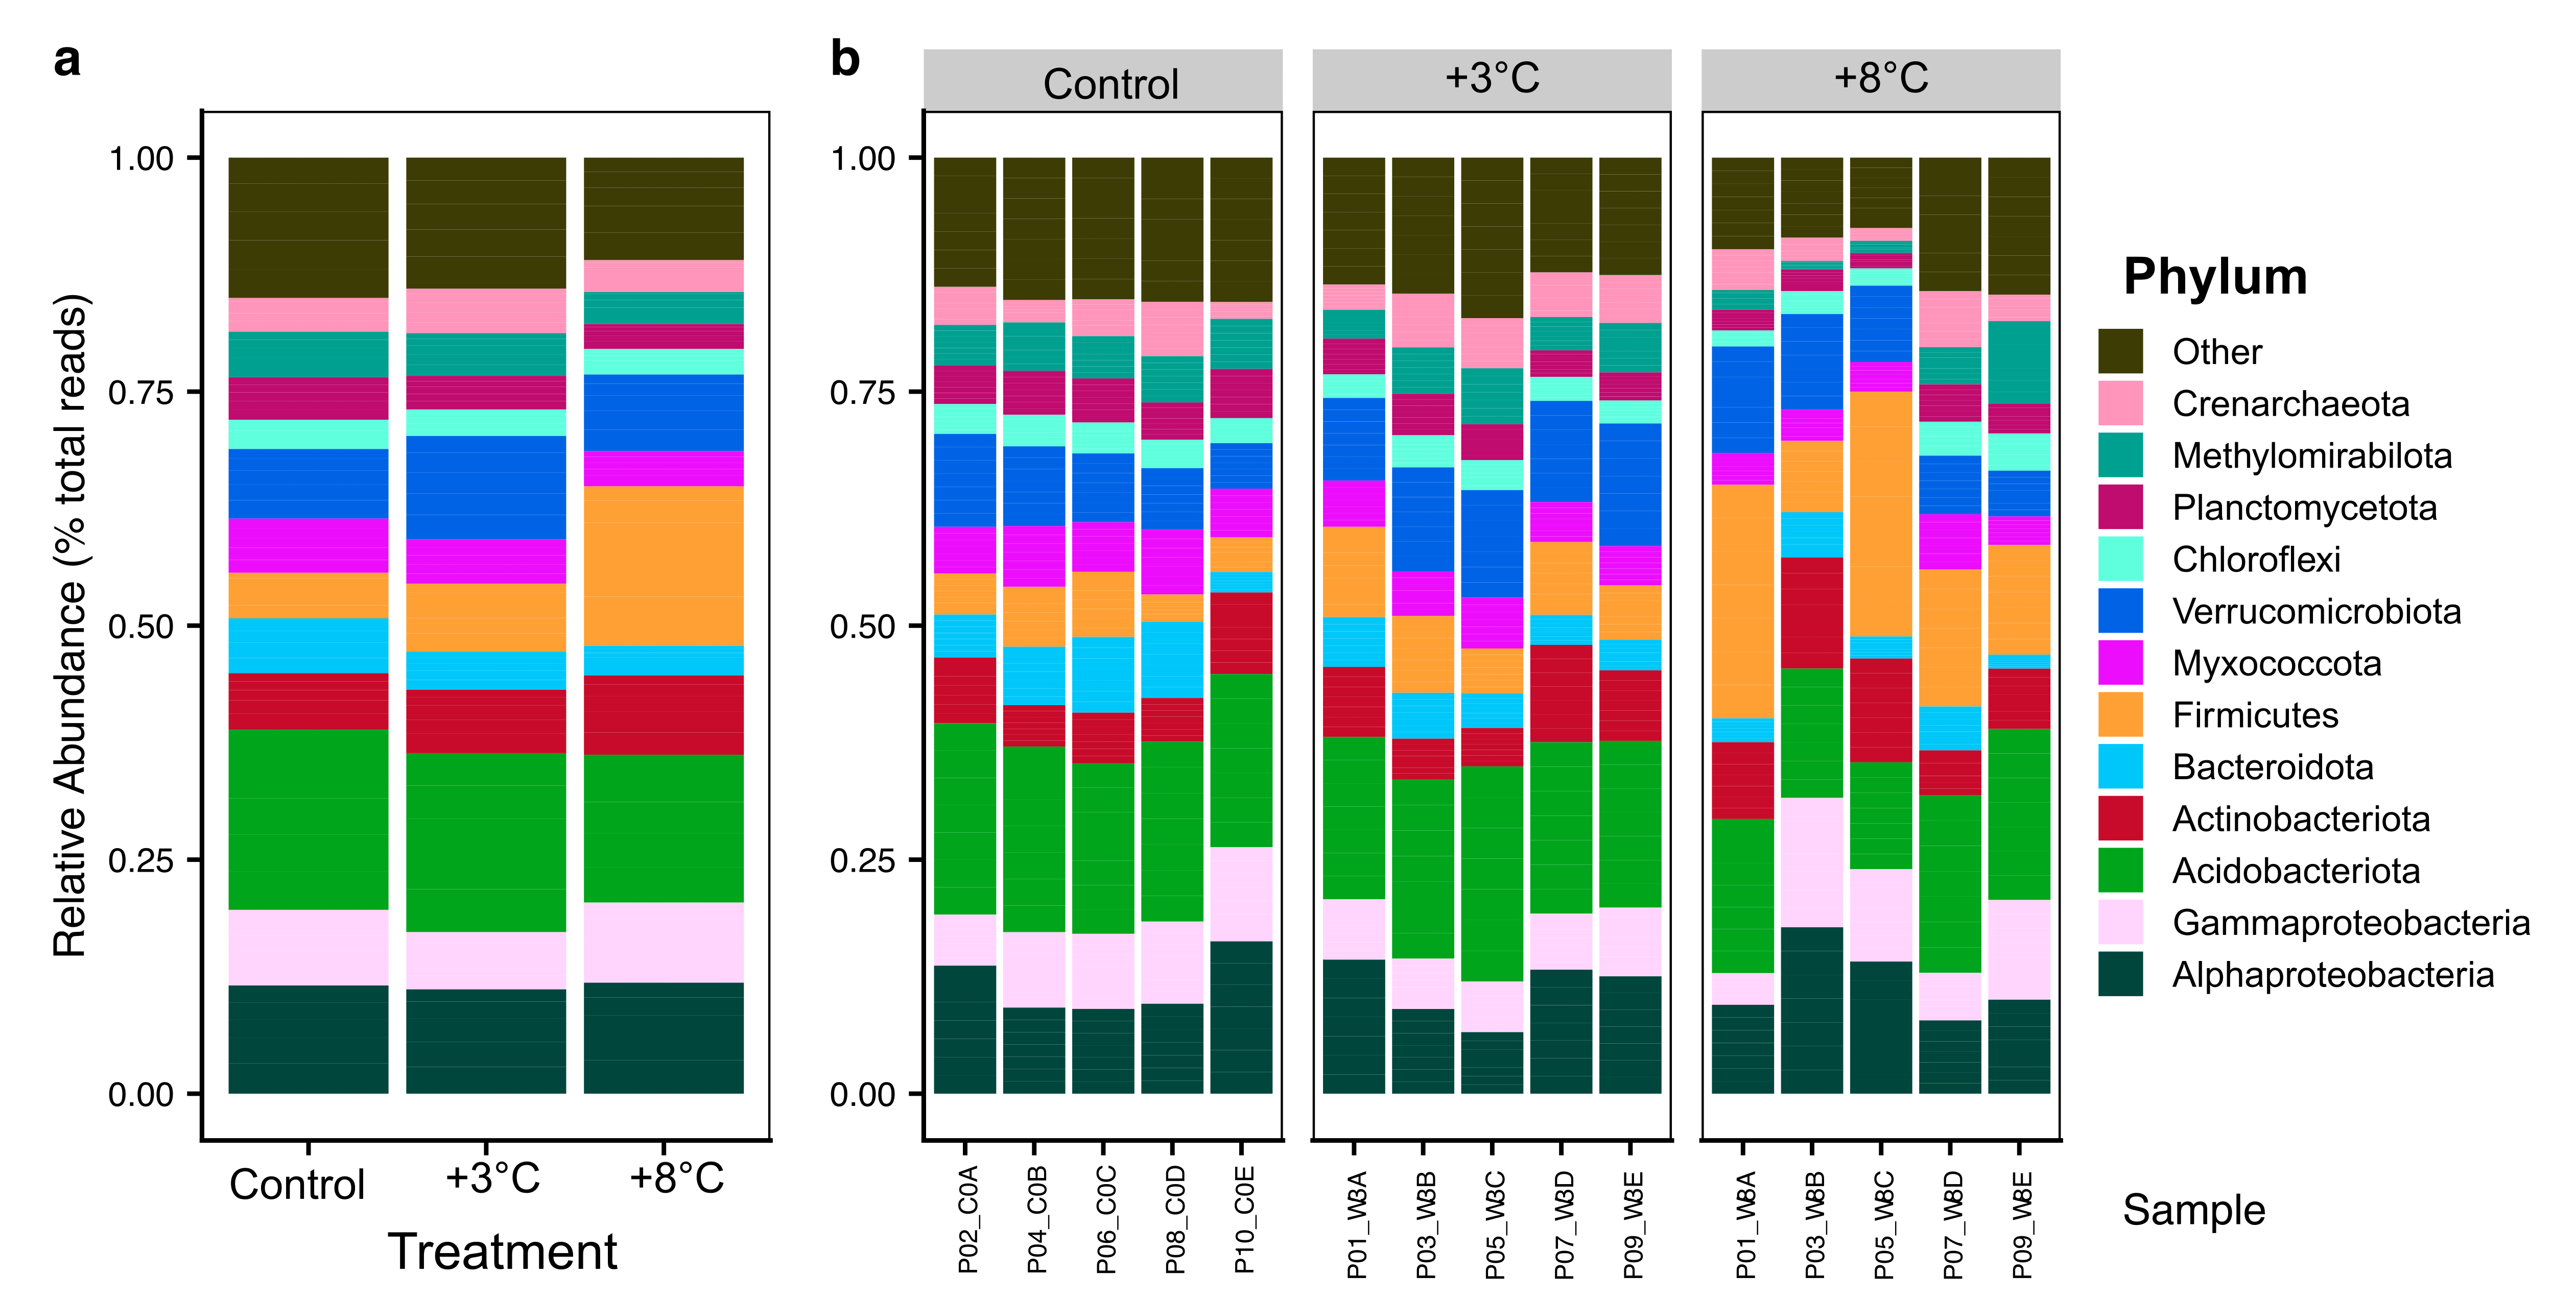
\includegraphics[width=0.87\textwidth,height=\textheight]{FIGURES/taxa_plots_main_ssu.png}

}

\caption{\textbf{Supplementary Figure 1 |} Top bacterial/archaeal phyla
(unfiltered data). (a) Collapsed by temperature treatment. (b) Samples
faceted by temperature treatment.}

\end{figure}

\begin{figure}

{\centering 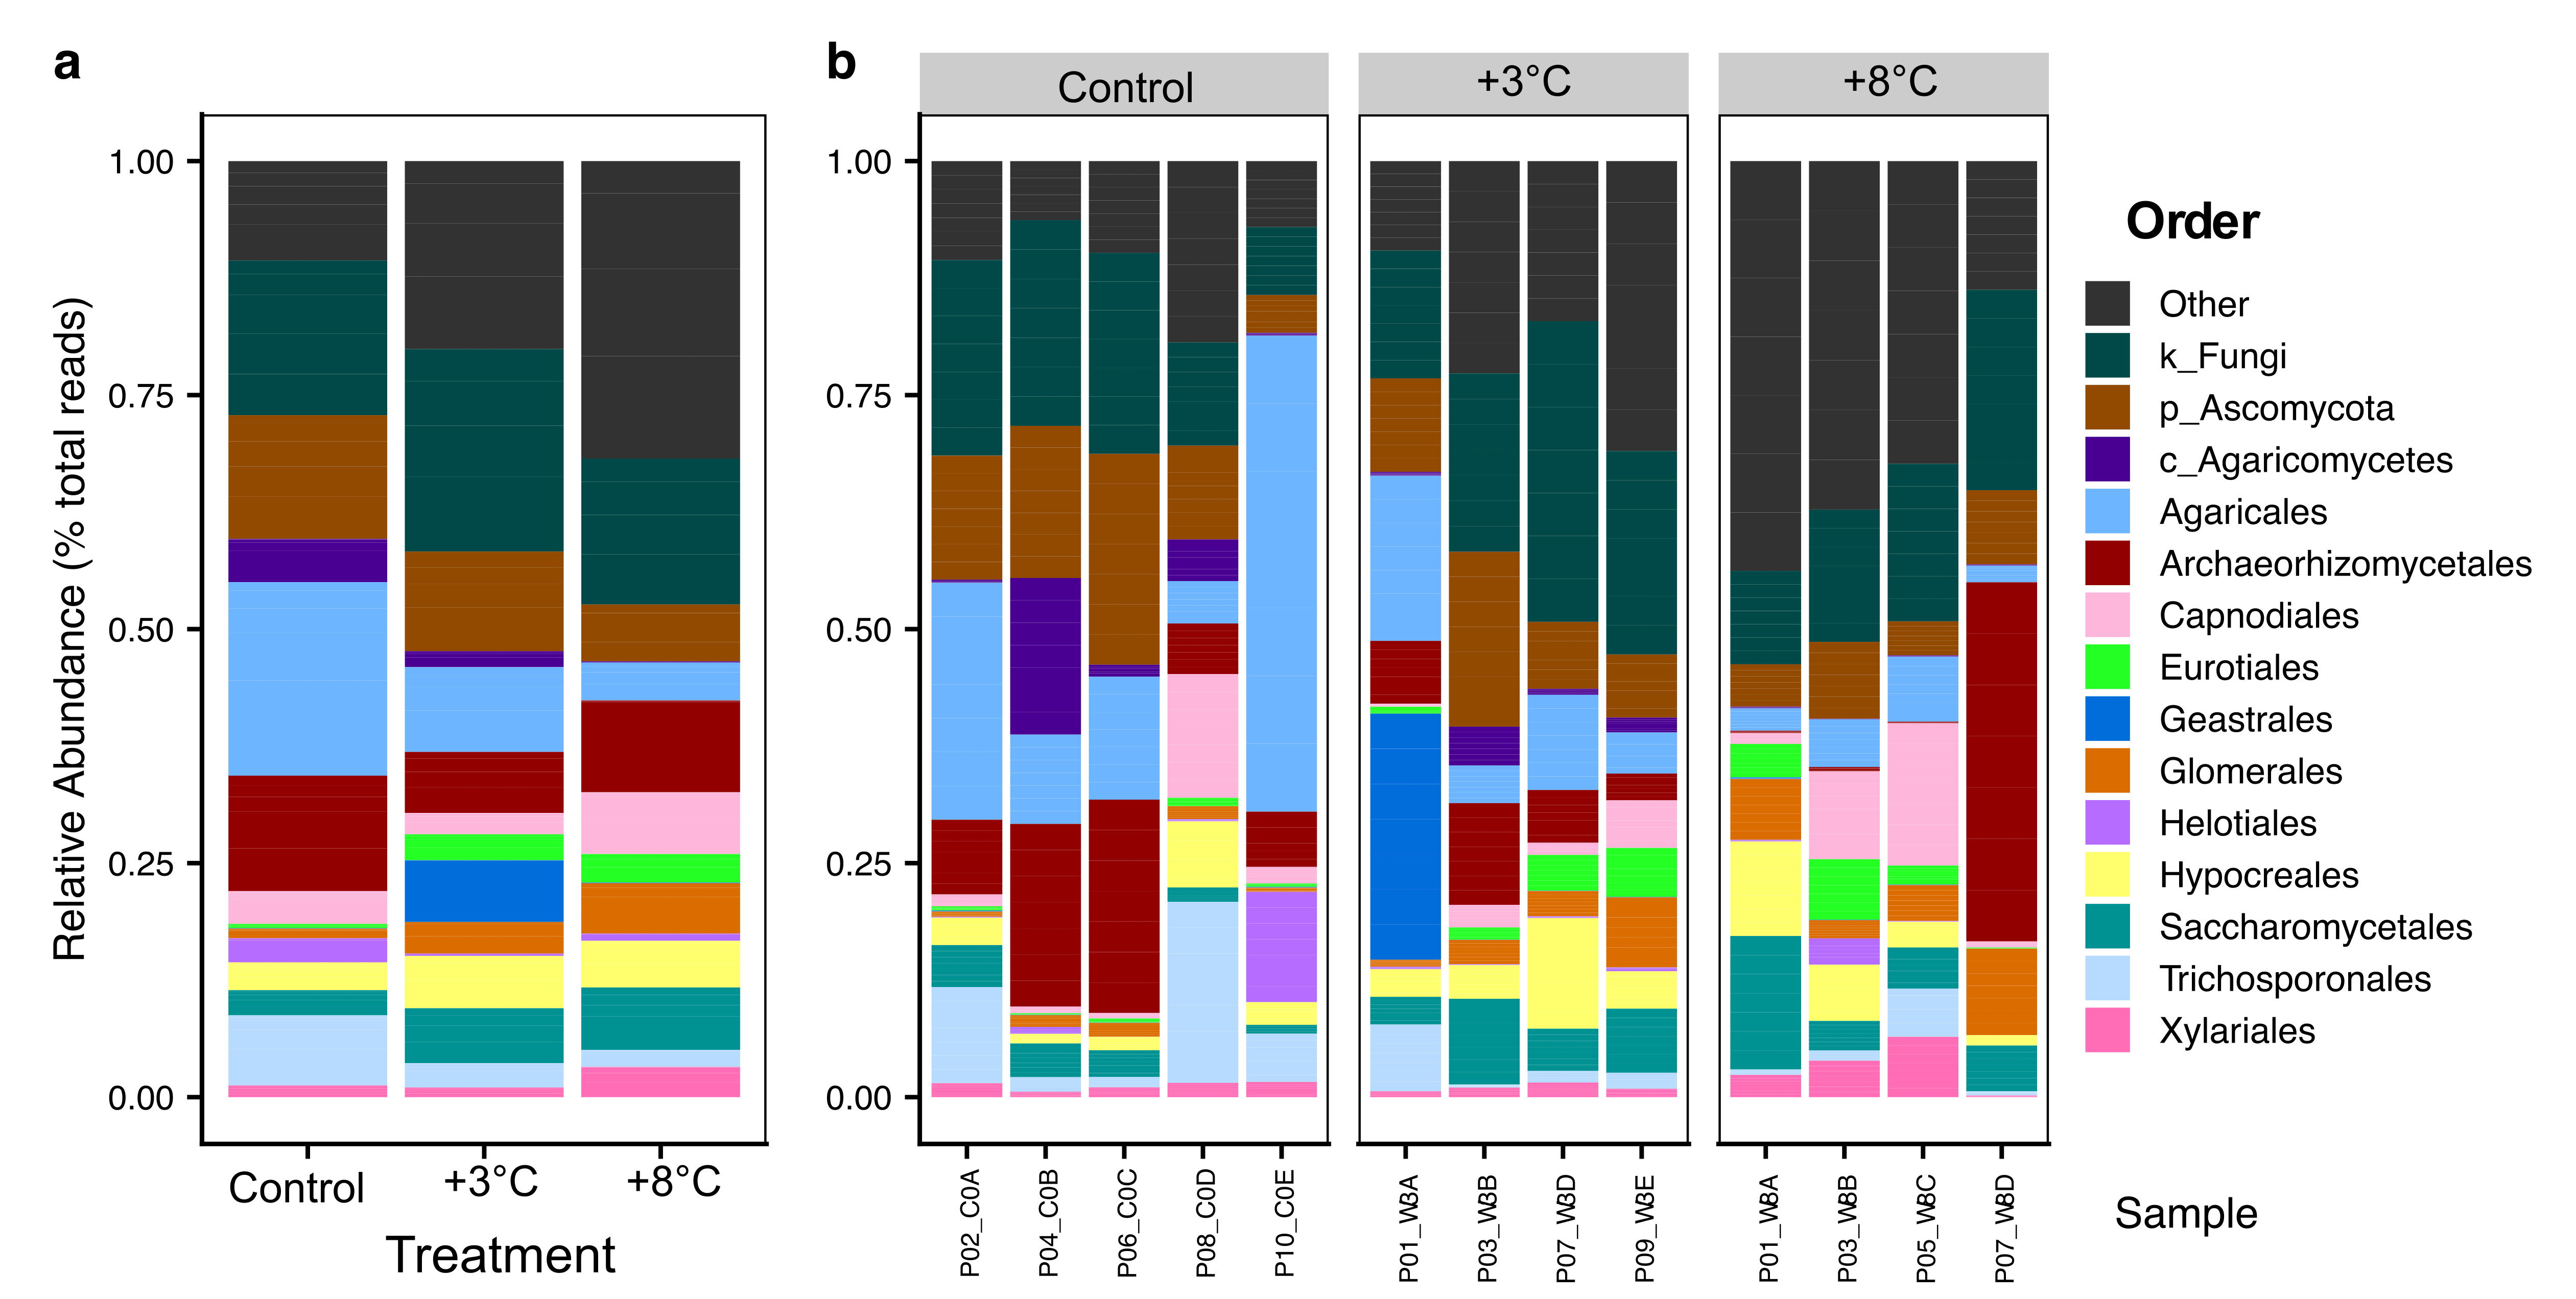
\includegraphics[width=0.87\textwidth,height=\textheight]{FIGURES/taxa_plots_main_its.png}

}

\caption{\textbf{Supplementary Figure 2 |} Top fungal orders (unfiltered
data). (a) Collapsed by temperature treatment. (b) Samples faceted by
temperature treatment.}

\end{figure}

\hypertarget{alpha-diversity-of-microbial-communities}{%
\subsection{Alpha diversity of microbial
communities}\label{alpha-diversity-of-microbial-communities}}

Shapiro-Wilk Normality and Bartlett tests indicated all data was
normally distributed except for Shannon exponential estimates of the 16S
rRNA PIME filtered data. Differences in alpha diversity assessed using
analysis of variance (ANOVA) followed by Tukey HSD post hoc tests
(normally distributed data) or Kruskal-Wallis followed by Dunn test with
Benjamini-Hochberg correction (non-normally distributed data).

See subsequent pages for results from the 16S rRNA data set
(\textbf{Supplementary Table 8}, \textbf{Supplementary Table 9}, and
\textbf{Supplementary Figure 3}) and the ITS data set
(\textbf{Supplementary Table 10}, \textbf{Supplementary Table 11}, and
\textbf{Supplementary Figure 4})

\newpage{}

\hypertarget{s-rrna-data-2}{%
\subsubsection{16S rRNA data}\label{s-rrna-data-2}}

\textbf{Supplementary Table 8} contains the results of alpha diversity
estimates for different filtering methods. In \textbf{Supplementary
Table 9} we report the results of the Shapiro-Wilk Normality and
Bartlett tests (and results of post-hoc analysis) for each Hill number.
\textbf{Supplementary Figure 3} contains alpha diversity plots comparing
the different filtering methods for Hill numbers.

\begin{table}[H]

\caption{\textbf{Supplementary Table 8 |} Hill numbers for 16S rRNA samples.}
\centering
\fontsize{7}{9}\selectfont
\begin{threeparttable}
\begin{tabular}[t]{lcccccccccccc}
\toprule
\multicolumn{1}{c}{ } & \multicolumn{4}{c}{Observed richness} & \multicolumn{4}{c}{Shannon exponential} & \multicolumn{4}{c}{Simpson multiplicative inverse} \\
\cmidrule(l{3pt}r{3pt}){2-5} \cmidrule(l{3pt}r{3pt}){6-9} \cmidrule(l{3pt}r{3pt}){10-13}
\textcolor{black}{\textbf{Sample}} & \textcolor{black}{\textbf{FULL}} & \textcolor{black}{\textbf{FILT}} & \textcolor{black}{\textbf{PERFect}} & \textcolor{black}{\textbf{PIME}} & \textcolor{black}{\textbf{FULL}} & \textcolor{black}{\textbf{FILT}} & \textcolor{black}{\textbf{PERFect}} & \textcolor{black}{\textbf{PIME}} & \textcolor{black}{\textbf{FULL}} & \textcolor{black}{\textbf{FILT}} & \textcolor{black}{\textbf{PERFect}} & \textcolor{black}{\textbf{PIME}}\\
\midrule
\cellcolor{gray!6}{P01\_W3A} & \cellcolor{gray!6}{2371} & \cellcolor{gray!6}{831} & \cellcolor{gray!6}{707} & \cellcolor{gray!6}{502} & \cellcolor{gray!6}{760.7} & \cellcolor{gray!6}{385.1} & \cellcolor{gray!6}{353.4} & \cellcolor{gray!6}{226.3} & \cellcolor{gray!6}{200.3} & \cellcolor{gray!6}{128.0} & \cellcolor{gray!6}{123.6} & \cellcolor{gray!6}{84.2}\\
P01\_W8A & 1610 & 620 & 563 & 322 & 236.1 & 127.8 & 126.5 & 59.2 & 25.5 & 18.9 & 19.1 & 12.0\\
\cellcolor{gray!6}{P02\_C0A} & \cellcolor{gray!6}{2272} & \cellcolor{gray!6}{884} & \cellcolor{gray!6}{737} & \cellcolor{gray!6}{590} & \cellcolor{gray!6}{781.1} & \cellcolor{gray!6}{437.1} & \cellcolor{gray!6}{397.4} & \cellcolor{gray!6}{291.2} & \cellcolor{gray!6}{261.5} & \cellcolor{gray!6}{178.5} & \cellcolor{gray!6}{171.6} & \cellcolor{gray!6}{129.3}\\
\addlinespace
P03\_W3B & 2356 & 922 & 764 & 596 & 686.8 & 373.7 & 337.3 & 235.0 & 159.4 & 108.7 & 103.8 & 75.8\\
\cellcolor{gray!6}{P03\_W8B} & \cellcolor{gray!6}{1575} & \cellcolor{gray!6}{422} & \cellcolor{gray!6}{411} & \cellcolor{gray!6}{224} & \cellcolor{gray!6}{501.0} & \cellcolor{gray!6}{181.0} & \cellcolor{gray!6}{211.9} & \cellcolor{gray!6}{90.1} & \cellcolor{gray!6}{153.3} & \cellcolor{gray!6}{69.2} & \cellcolor{gray!6}{82.6} & \cellcolor{gray!6}{38.6}\\
P04\_C0B & 2040 & 802 & 663 & 570 & 797.8 & 439.4 & 388.4 & 309.2 & 272.0 & 178.8 & 166.8 & 130.7\\
\addlinespace
\cellcolor{gray!6}{P05\_W3C} & \cellcolor{gray!6}{1663} & \cellcolor{gray!6}{680} & \cellcolor{gray!6}{574} & \cellcolor{gray!6}{499} & \cellcolor{gray!6}{578.8} & \cellcolor{gray!6}{329.4} & \cellcolor{gray!6}{299.2} & \cellcolor{gray!6}{246.1} & \cellcolor{gray!6}{201.2} & \cellcolor{gray!6}{139.5} & \cellcolor{gray!6}{132.6} & \cellcolor{gray!6}{111.0}\\
P05\_W8C & 2124 & 572 & 661 & 289 & 307.3 & 102.4 & 146.9 & 47.9 & 27.3 & 14.9 & 18.5 & 9.6\\
\cellcolor{gray!6}{P06\_C0C} & \cellcolor{gray!6}{3065} & \cellcolor{gray!6}{1011} & \cellcolor{gray!6}{857} & \cellcolor{gray!6}{664} & \cellcolor{gray!6}{1098.4} & \cellcolor{gray!6}{518.7} & \cellcolor{gray!6}{481.3} & \cellcolor{gray!6}{324.7} & \cellcolor{gray!6}{309.4} & \cellcolor{gray!6}{182.0} & \cellcolor{gray!6}{179.7} & \cellcolor{gray!6}{120.6}\\
\addlinespace
P07\_W3D & 2010 & 843 & 725 & 516 & 598.8 & 353.4 & 327.5 & 208.0 & 146.8 & 103.7 & 99.7 & 67.5\\
\cellcolor{gray!6}{P07\_W8D} & \cellcolor{gray!6}{2157} & \cellcolor{gray!6}{771} & \cellcolor{gray!6}{671} & \cellcolor{gray!6}{276} & \cellcolor{gray!6}{560.8} & \cellcolor{gray!6}{284.2} & \cellcolor{gray!6}{270.3} & \cellcolor{gray!6}{88.1} & \cellcolor{gray!6}{91.5} & \cellcolor{gray!6}{60.2} & \cellcolor{gray!6}{60.2} & \cellcolor{gray!6}{24.4}\\
P08\_C0D & 2441 & 813 & 681 & 594 & 973.3 & 464.8 & 419.8 & 331.3 & 394.2 & 230.0 & 220.5 & 168.7\\
\addlinespace
\cellcolor{gray!6}{P09\_W3E} & \cellcolor{gray!6}{2386} & \cellcolor{gray!6}{874} & \cellcolor{gray!6}{751} & \cellcolor{gray!6}{563} & \cellcolor{gray!6}{680.1} & \cellcolor{gray!6}{352.7} & \cellcolor{gray!6}{334.5} & \cellcolor{gray!6}{224.4} & \cellcolor{gray!6}{168.5} & \cellcolor{gray!6}{110.3} & \cellcolor{gray!6}{109.4} & \cellcolor{gray!6}{76.5}\\
P09\_W8E & 813 & 376 & 332 & 170 & 375.3 & 165.6 & 149.9 & 67.9 & 120.2 & 55.7 & 56.8 & 26.4\\
\cellcolor{gray!6}{P10\_C0E} & \cellcolor{gray!6}{2066} & \cellcolor{gray!6}{670} & \cellcolor{gray!6}{571} & \cellcolor{gray!6}{491} & \cellcolor{gray!6}{886.8} & \cellcolor{gray!6}{416.5} & \cellcolor{gray!6}{379.4} & \cellcolor{gray!6}{298.3} & \cellcolor{gray!6}{427.6} & \cellcolor{gray!6}{242.8} & \cellcolor{gray!6}{231.4} & \cellcolor{gray!6}{174.7}\\
\bottomrule
\end{tabular}
\begin{tablenotes}
\item FULL = unfiltered data set; FILT = arbitrary filtering where nreads > 5 and prevalence > 20\%; PERFect = PERFect filtering; PIME = PIME filtering
\end{tablenotes}
\end{threeparttable}
\end{table}

\begin{table}[H]

\caption{\textbf{Supplementary Table 9 |} Summary of 16S rRNA significant tests. Posthoc p-values adjusted for multiple comparisons.}
\centering
\fontsize{8}{10}\selectfont
\begin{threeparttable}
\begin{tabular}[t]{lccclcc}
\toprule
\textcolor{black}{\textbf{metric\textsuperscript{1}}} & \textcolor{black}{\textbf{data set\textsuperscript{2}}} & \textcolor{black}{\textbf{pval shap\textsuperscript{3}}} & \textcolor{black}{\textbf{pval bart\textsuperscript{4}}} & \textcolor{black}{\textbf{method\textsuperscript{5}}} & \textcolor{black}{\textbf{posthoc method\textsuperscript{6}}} & \textcolor{black}{\textbf{posthoc pval\textsuperscript{7}}}\\
\midrule
\cellcolor{gray!6}{Observed} & \cellcolor{gray!6}{FULL} & \cellcolor{gray!6}{0.268} & \cellcolor{gray!6}{0.599} & \cellcolor{gray!6}{ANOVA} & \cellcolor{gray!6}{Tukey post-hoc test} & \cellcolor{gray!6}{6.05e-02}\\
Observed & FILT & 0.367 & 0.585 & ANOVA & Tukey post-hoc test & 6.08e-03\\
\cellcolor{gray!6}{Observed} & \cellcolor{gray!6}{PERFect} & \cellcolor{gray!6}{0.191} & \cellcolor{gray!6}{0.437} & \cellcolor{gray!6}{ANOVA} & \cellcolor{gray!6}{Tukey post-hoc test} & \cellcolor{gray!6}{5.05e-02}\\
Observed & PIME & 0.055 & 0.755 & ANOVA & Tukey post-hoc test & 1.40e-06\\
\addlinespace
\cellcolor{gray!6}{Shannon exponential} & \cellcolor{gray!6}{FULL} & \cellcolor{gray!6}{0.994} & \cellcolor{gray!6}{0.490} & \cellcolor{gray!6}{ANOVA} & \cellcolor{gray!6}{Tukey post-hoc test} & \cellcolor{gray!6}{6.27e-05}\\
Shannon exponential & FILT & 0.230 & 0.107 & ANOVA & Tukey post-hoc test & 2.60e-06\\
\cellcolor{gray!6}{Shannon exponential} & \cellcolor{gray!6}{PERFect} & \cellcolor{gray!6}{0.331} & \cellcolor{gray!6}{0.159} & \cellcolor{gray!6}{ANOVA} & \cellcolor{gray!6}{Tukey post-hoc test} & \cellcolor{gray!6}{7.10e-06}\\
Shannon exponential & PIME & 0.037 & 0.880 & Kruskal-Wallis & Dunn test & 1.93e-03\\
\addlinespace
\cellcolor{gray!6}{Inverse Simpson} & \cellcolor{gray!6}{FULL} & \cellcolor{gray!6}{0.584} & \cellcolor{gray!6}{0.155} & \cellcolor{gray!6}{ANOVA} & \cellcolor{gray!6}{Tukey post-hoc test} & \cellcolor{gray!6}{4.67e-05}\\
Inverse Simpson & FILT & 0.673 & 0.413 & ANOVA & Tukey post-hoc test & 1.30e-06\\
\cellcolor{gray!6}{Inverse Simpson} & \cellcolor{gray!6}{PERFect} & \cellcolor{gray!6}{0.747} & \cellcolor{gray!6}{0.348} & \cellcolor{gray!6}{ANOVA} & \cellcolor{gray!6}{Tukey post-hoc test} & \cellcolor{gray!6}{3.20e-06}\\
Inverse Simpson & PIME & 0.370 & 0.371 & ANOVA & Tukey post-hoc test & 1.00e-06\\
\bottomrule
\end{tabular}
\begin{tablenotes}[para]
\item \textbf{Column descriptions. } 
\item 
\item[1] metric: Hill number; 
\item[2] data set: FULL = unfiltered data set; FILT = arbitrary filtering where nreads > 5 and prevalence > 20\%; PERFect = PERFect filtering; PIME = PIME filtering
\item[3] pval\_shap: p-value of Shapiro-Wilk Normality test; 
\item[4] pval\_bart: p-value of Bartlett Test of Homogeneity of Variances; 
\item[5] method: Selected significance test; 
\item[6] posthoc method: Selected posthoc test; 
\item[7] posthoc pval: Posthoc p-value; 
\end{tablenotes}
\end{threeparttable}
\end{table}

\newpage{}

\begin{figure}

{\centering 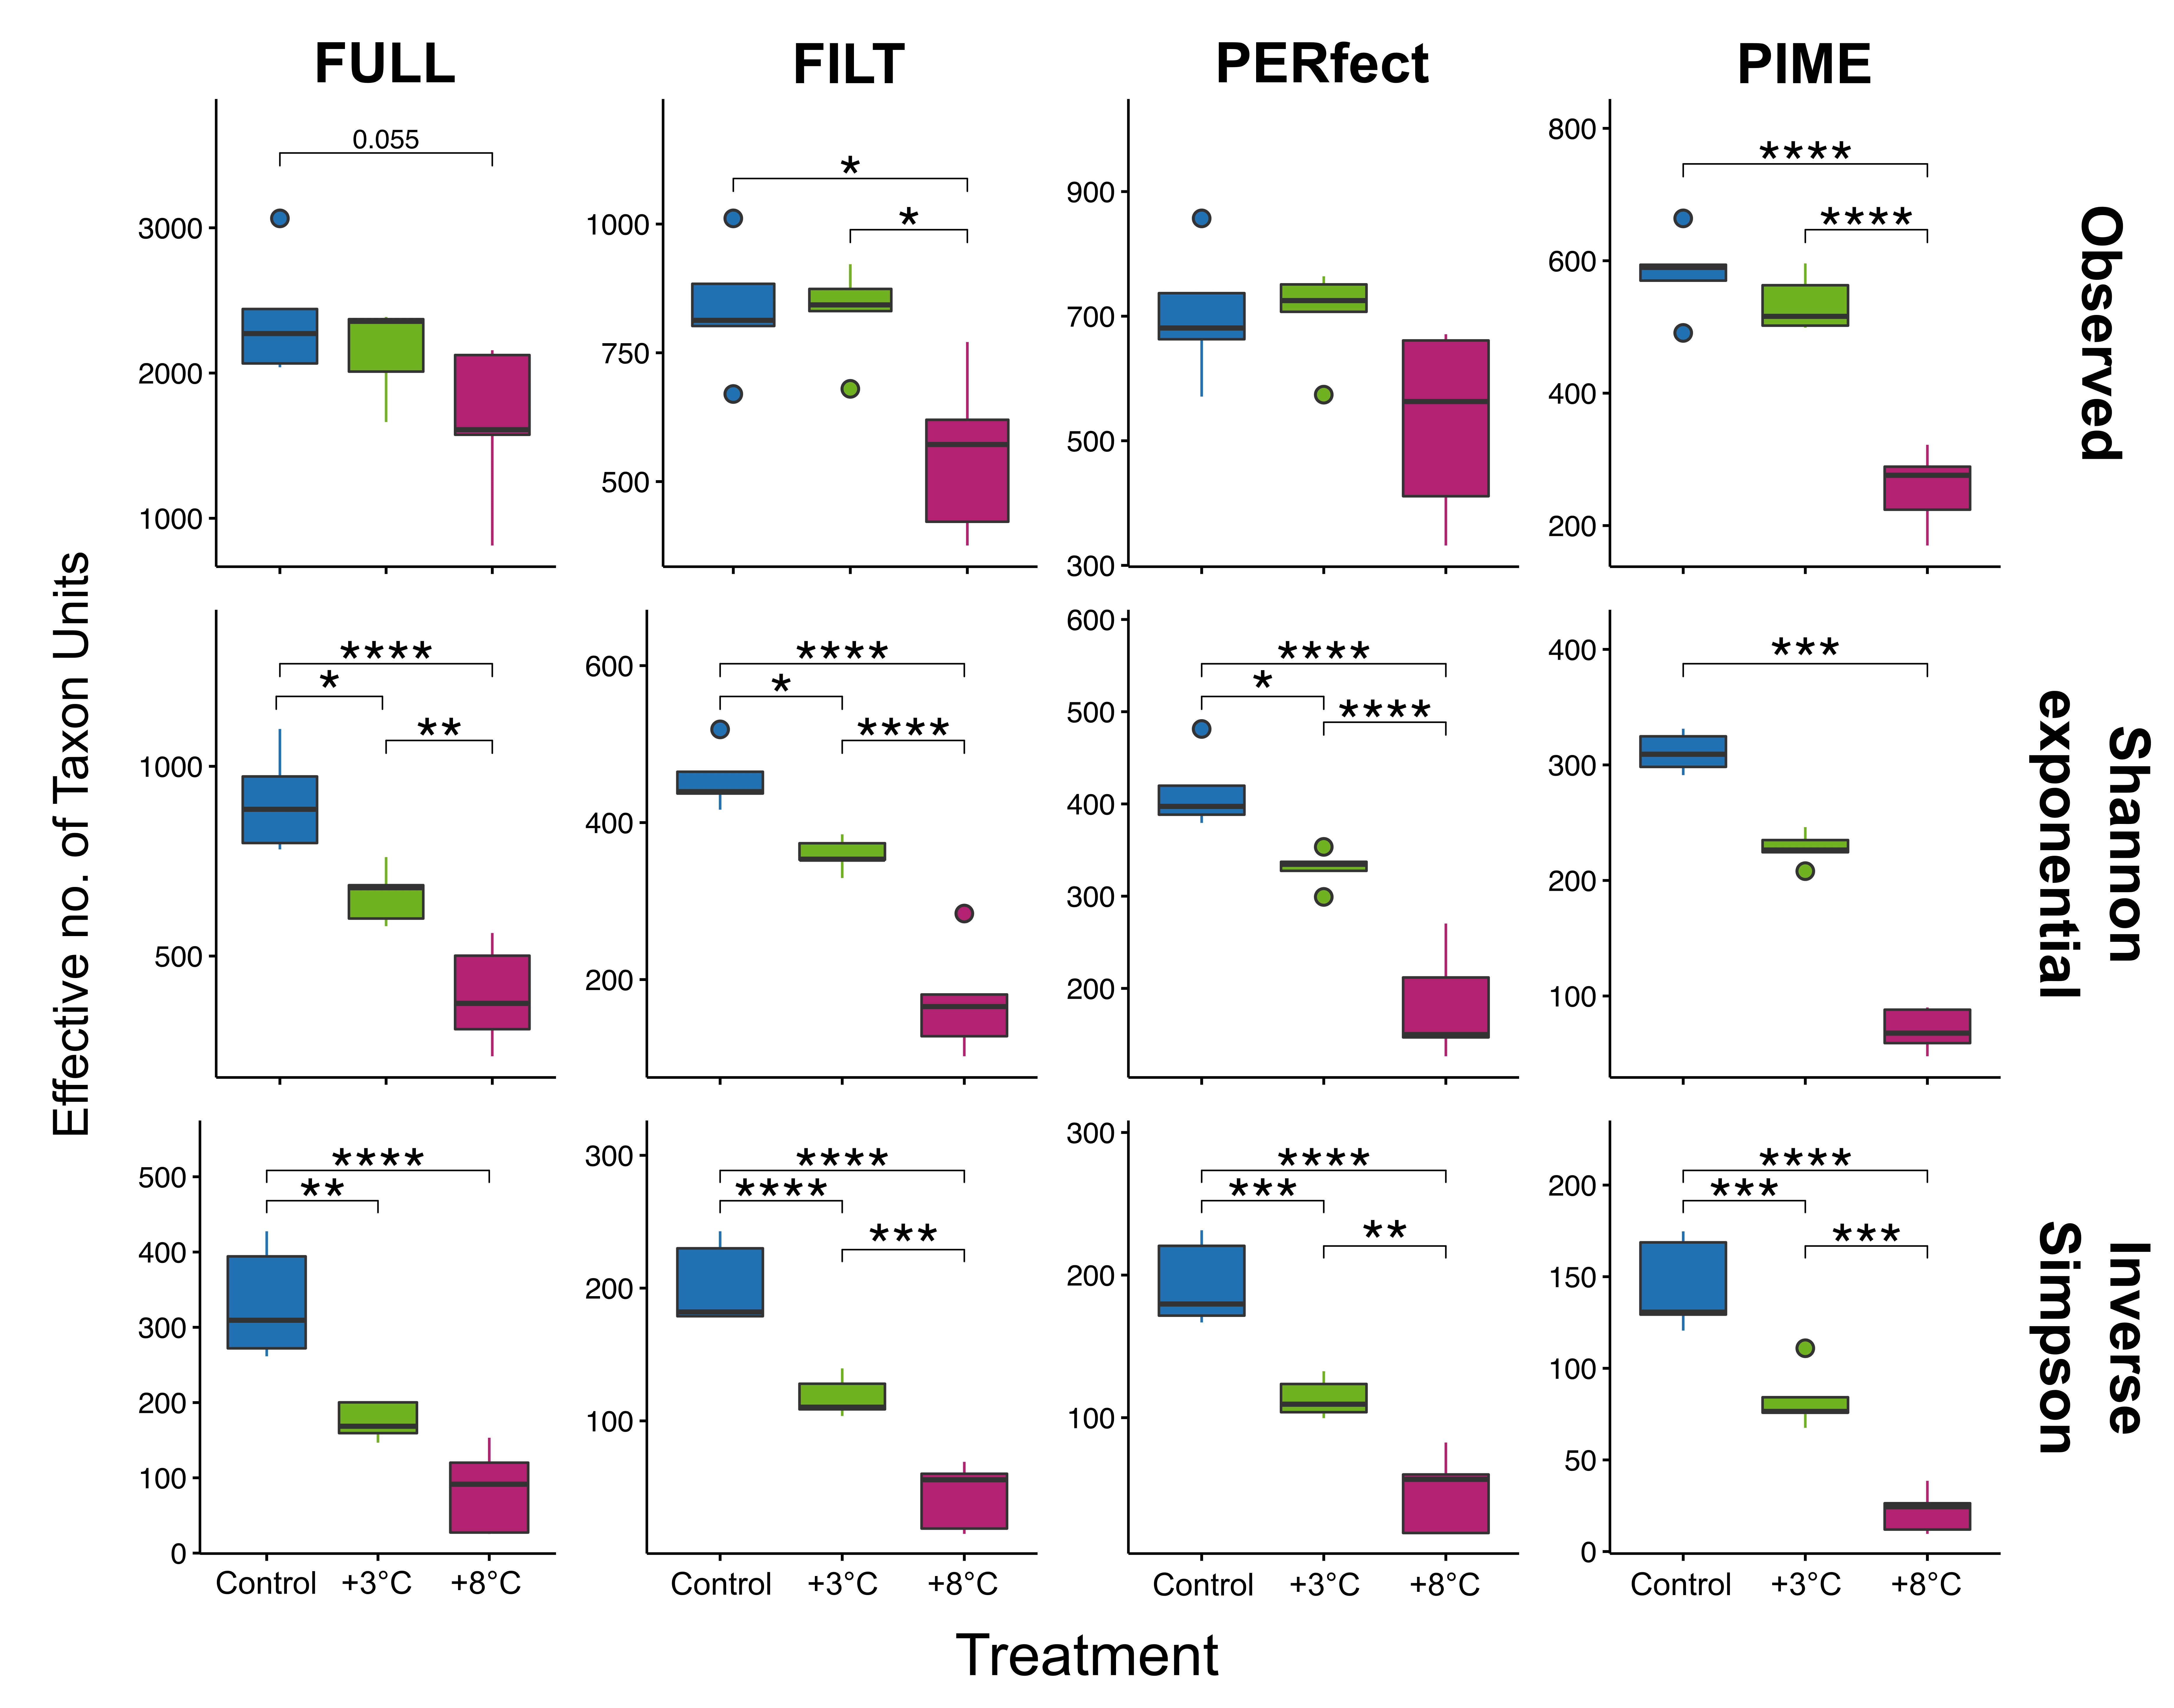
\includegraphics[width=1\textwidth,height=\textheight]{FIGURES/ssu_supp_alpha_div.png}

}

\caption{\textbf{Supplementary Figure 3 |} Alpha diversity estimates of
16S rRNA communities. The centre line of each box plot represents the
median, the lower and upper hinges represent the first and third
quartiles and whiskers represent + 1.5 the interquartile range.
Shapiro-Wilk Normality Test and Bartlett Test of Homogeneity of
Variances normality tests indicated all data was normally distributed
except for Shannon exponential estimates of the PIME filtered data.
Differences in alpha diversity assessed using analysis of variance
(ANOVA) followed by Tukey HSD post hoc tests (normally distributed data)
or Kruskal-Wallis followed by Dunn test with Benjamini-Hochberg
correction (non-normally distributed data). Only significant differences
(p-values adjusted for multiple comparisons) between treatments and
controls are shown in plots, where n = 5 for each treatment.}

\end{figure}

\newpage{}

\hypertarget{its-data-2}{%
\subsubsection{ITS data}\label{its-data-2}}

\textbf{Supplementary Table 10} contains the results of alpha diversity
estimates for different filtering methods. In \textbf{Supplementary
Table 11} we report the results of the Shapiro-Wilk Normality and
Bartlett tests (and results of post-hoc analysis) for each Hill number.
\textbf{Supplementary Figure 4} contains alpha diversity plots comparing
the different filtering methods for Hill numbers.

\begin{table}[H]

\caption{\textbf{Supplementary Table 10 |} Hill numbers for ITS samples.}
\centering
\fontsize{7}{9}\selectfont
\begin{threeparttable}
\begin{tabular}[t]{lcccccccccccc}
\toprule
\multicolumn{1}{c}{ } & \multicolumn{4}{c}{Observed richness} & \multicolumn{4}{c}{Shannon exponential} & \multicolumn{4}{c}{Simpson multiplicative inverse} \\
\cmidrule(l{3pt}r{3pt}){2-5} \cmidrule(l{3pt}r{3pt}){6-9} \cmidrule(l{3pt}r{3pt}){10-13}
\textcolor{black}{\textbf{Sample}} & \textcolor{black}{\textbf{FULL}} & \textcolor{black}{\textbf{FILT}} & \textcolor{black}{\textbf{PERFect}} & \textcolor{black}{\textbf{PIME}} & \textcolor{black}{\textbf{FULL}} & \textcolor{black}{\textbf{FILT}} & \textcolor{black}{\textbf{PERFect}} & \textcolor{black}{\textbf{PIME}} & \textcolor{black}{\textbf{FULL}} & \textcolor{black}{\textbf{FILT}} & \textcolor{black}{\textbf{PERFect}} & \textcolor{black}{\textbf{PIME}}\\
\midrule
\cellcolor{gray!6}{P01\_W3A} & \cellcolor{gray!6}{945} & \cellcolor{gray!6}{499} & \cellcolor{gray!6}{148} & \cellcolor{gray!6}{181} & \cellcolor{gray!6}{55.9} & \cellcolor{gray!6}{33.8} & \cellcolor{gray!6}{18.5} & \cellcolor{gray!6}{14.8} & \cellcolor{gray!6}{10.7} & \cellcolor{gray!6}{8.4} & \cellcolor{gray!6}{6.8} & \cellcolor{gray!6}{5.6}\\
P01\_W8A & 719 & 344 & 98 & 123 & 141.5 & 79.0 & 31.8 & 31.6 & 42.4 & 28.1 & 17.3 & 12.5\\
\cellcolor{gray!6}{P02\_C0A} & \cellcolor{gray!6}{1011} & \cellcolor{gray!6}{494} & \cellcolor{gray!6}{147} & \cellcolor{gray!6}{238} & \cellcolor{gray!6}{112.5} & \cellcolor{gray!6}{64.0} & \cellcolor{gray!6}{38.1} & \cellcolor{gray!6}{43.3} & \cellcolor{gray!6}{36.1} & \cellcolor{gray!6}{26.2} & \cellcolor{gray!6}{21.9} & \cellcolor{gray!6}{19.9}\\
\addlinespace
P03\_W3B & 765 & 423 & 136 & 196 & 132.9 & 83.0 & 45.7 & 56.5 & 44.1 & 29.1 & 24.4 & 26.9\\
\cellcolor{gray!6}{P03\_W8B} & \cellcolor{gray!6}{349} & \cellcolor{gray!6}{204} & \cellcolor{gray!6}{64} & \cellcolor{gray!6}{109} & \cellcolor{gray!6}{112.1} & \cellcolor{gray!6}{72.2} & \cellcolor{gray!6}{26.2} & \cellcolor{gray!6}{42.8} & \cellcolor{gray!6}{49.0} & \cellcolor{gray!6}{36.4} & \cellcolor{gray!6}{17.8} & \cellcolor{gray!6}{23.7}\\
P04\_C0B & 1017 & 471 & 161 & 229 & 60.9 & 43.3 & 25.2 & 39.5 & 17.6 & 15.5 & 12.5 & 20.6\\
\addlinespace
\cellcolor{gray!6}{P05\_W8C} & \cellcolor{gray!6}{616} & \cellcolor{gray!6}{296} & \cellcolor{gray!6}{90} & \cellcolor{gray!6}{131} & \cellcolor{gray!6}{157.5} & \cellcolor{gray!6}{76.6} & \cellcolor{gray!6}{34.2} & \cellcolor{gray!6}{35.1} & \cellcolor{gray!6}{41.8} & \cellcolor{gray!6}{20.7} & \cellcolor{gray!6}{15.3} & \cellcolor{gray!6}{11.5}\\
P06\_C0C & 954 & 486 & 157 & 246 & 99.5 & 58.4 & 34.2 & 35.2 & 23.9 & 16.5 & 14.8 & 13.1\\
\addlinespace
\cellcolor{gray!6}{P07\_W3D} & \cellcolor{gray!6}{867} & \cellcolor{gray!6}{492} & \cellcolor{gray!6}{147} & \cellcolor{gray!6}{205} & \cellcolor{gray!6}{160.4} & \cellcolor{gray!6}{102.9} & \cellcolor{gray!6}{46.3} & \cellcolor{gray!6}{48.0} & \cellcolor{gray!6}{56.2} & \cellcolor{gray!6}{42.8} & \cellcolor{gray!6}{27.2} & \cellcolor{gray!6}{22.5}\\
P07\_W8D & 335 & 223 & 76 & 97 & 35.0 & 28.0 & 16.9 & 18.1 & 13.7 & 12.3 & 9.1 & 9.9\\
\cellcolor{gray!6}{P08\_C0D} & \cellcolor{gray!6}{702} & \cellcolor{gray!6}{345} & \cellcolor{gray!6}{105} & \cellcolor{gray!6}{198} & \cellcolor{gray!6}{87.2} & \cellcolor{gray!6}{46.7} & \cellcolor{gray!6}{25.7} & \cellcolor{gray!6}{30.7} & \cellcolor{gray!6}{25.5} & \cellcolor{gray!6}{17.9} & \cellcolor{gray!6}{14.2} & \cellcolor{gray!6}{14.2}\\
\addlinespace
P09\_W3E & 745 & 390 & 118 & 196 & 232.7 & 133.6 & 51.9 & 66.6 & 96.0 & 61.7 & 33.9 & 34.9\\
\cellcolor{gray!6}{P10\_C0E} & \cellcolor{gray!6}{812} & \cellcolor{gray!6}{404} & \cellcolor{gray!6}{143} & \cellcolor{gray!6}{203} & \cellcolor{gray!6}{24.6} & \cellcolor{gray!6}{14.7} & \cellcolor{gray!6}{11.1} & \cellcolor{gray!6}{8.1} & \cellcolor{gray!6}{4.9} & \cellcolor{gray!6}{4.0} & \cellcolor{gray!6}{3.8} & \cellcolor{gray!6}{2.5}\\
\bottomrule
\end{tabular}
\begin{tablenotes}
\item FULL = unfiltered data set; FILT = arbitrary filtering where nreads > 5 and prevalence > 20\%; PERFect = PERFect filtering; PIME = PIME filtering
\end{tablenotes}
\end{threeparttable}
\end{table}

\begin{table}[H]

\caption{\textbf{Supplementary Table 11 |} Summary of ITS significant tests. Posthoc p-values adjusted for multiple comparisons.}
\centering
\fontsize{8}{10}\selectfont
\begin{threeparttable}
\begin{tabular}[t]{lccclcc}
\toprule
\textcolor{black}{\textbf{metric\textsuperscript{1}}} & \textcolor{black}{\textbf{data set\textsuperscript{2}}} & \textcolor{black}{\textbf{pval shap\textsuperscript{3}}} & \textcolor{black}{\textbf{pval bart\textsuperscript{4}}} & \textcolor{black}{\textbf{method\textsuperscript{5}}} & \textcolor{black}{\textbf{posthoc method\textsuperscript{6}}} & \textcolor{black}{\textbf{posthoc pval\textsuperscript{7}}}\\
\midrule
\cellcolor{gray!6}{Observed} & \cellcolor{gray!6}{FULL} & \cellcolor{gray!6}{0.128} & \cellcolor{gray!6}{0.516} & \cellcolor{gray!6}{ANOVA} & \cellcolor{gray!6}{Tukey post-hoc test} & \cellcolor{gray!6}{6.14e-03}\\
Observed & FILT & 0.115 & 0.938 & ANOVA & Tukey post-hoc test & 2.36e-03\\
\cellcolor{gray!6}{Observed} & \cellcolor{gray!6}{PERFect} & \cellcolor{gray!6}{0.162} & \cellcolor{gray!6}{0.667} & \cellcolor{gray!6}{ANOVA} & \cellcolor{gray!6}{Tukey post-hoc test} & \cellcolor{gray!6}{1.09e-03}\\
Observed & PIME & 0.134 & 0.454 & ANOVA & Tukey post-hoc test & 7.40e-06\\
\addlinespace
\cellcolor{gray!6}{Shannon exponential} & \cellcolor{gray!6}{FULL} & \cellcolor{gray!6}{0.846} & \cellcolor{gray!6}{0.445} & \cellcolor{gray!6}{ANOVA} & \cellcolor{gray!6}{Tukey post-hoc test} & \cellcolor{gray!6}{2.21e-01}\\
Shannon exponential & FILT & 0.934 & 0.363 & ANOVA & Tukey post-hoc test & 1.39e-01\\
\cellcolor{gray!6}{Shannon exponential} & \cellcolor{gray!6}{PERFect} & \cellcolor{gray!6}{0.919} & \cellcolor{gray!6}{0.555} & \cellcolor{gray!6}{ANOVA} & \cellcolor{gray!6}{Tukey post-hoc test} & \cellcolor{gray!6}{1.87e-01}\\
Shannon exponential & PIME & 0.972 & 0.436 & ANOVA & Tukey post-hoc test & 3.46e-01\\
\addlinespace
\cellcolor{gray!6}{Inverse Simpson} & \cellcolor{gray!6}{FULL} & \cellcolor{gray!6}{0.184} & \cellcolor{gray!6}{0.126} & \cellcolor{gray!6}{ANOVA} & \cellcolor{gray!6}{Tukey post-hoc test} & \cellcolor{gray!6}{1.82e-01}\\
Inverse Simpson & FILT & 0.349 & 0.159 & ANOVA & Tukey post-hoc test & 1.83e-01\\
\cellcolor{gray!6}{Inverse Simpson} & \cellcolor{gray!6}{PERFect} & \cellcolor{gray!6}{0.961} & \cellcolor{gray!6}{0.236} & \cellcolor{gray!6}{ANOVA} & \cellcolor{gray!6}{Tukey post-hoc test} & \cellcolor{gray!6}{2.05e-01}\\
Inverse Simpson & PIME & 0.955 & 0.477 & ANOVA & Tukey post-hoc test & 3.42e-01\\
\bottomrule
\end{tabular}
\begin{tablenotes}[para]
\item \textbf{Column descriptions. } 
\item 
\item[1] metric: Hill number; 
\item[2] data set: FULL = unfiltered data set; FILT = arbitrary filtering where nreads > 5 and prevalence > 20\%; PERFect = PERFect filtering; PIME = PIME filtering
\item[3] pval\_shap: p-value of Shapiro-Wilk Normality test; 
\item[4] pval\_bart: p-value of Bartlett Test of Homogeneity of Variances; 
\item[5] method: Selected significance test; 
\item[6] posthoc method: Selected posthoc test; 
\item[7] posthoc pval: Posthoc p-value; 
\end{tablenotes}
\end{threeparttable}
\end{table}

\newpage{}

\begin{figure}

{\centering 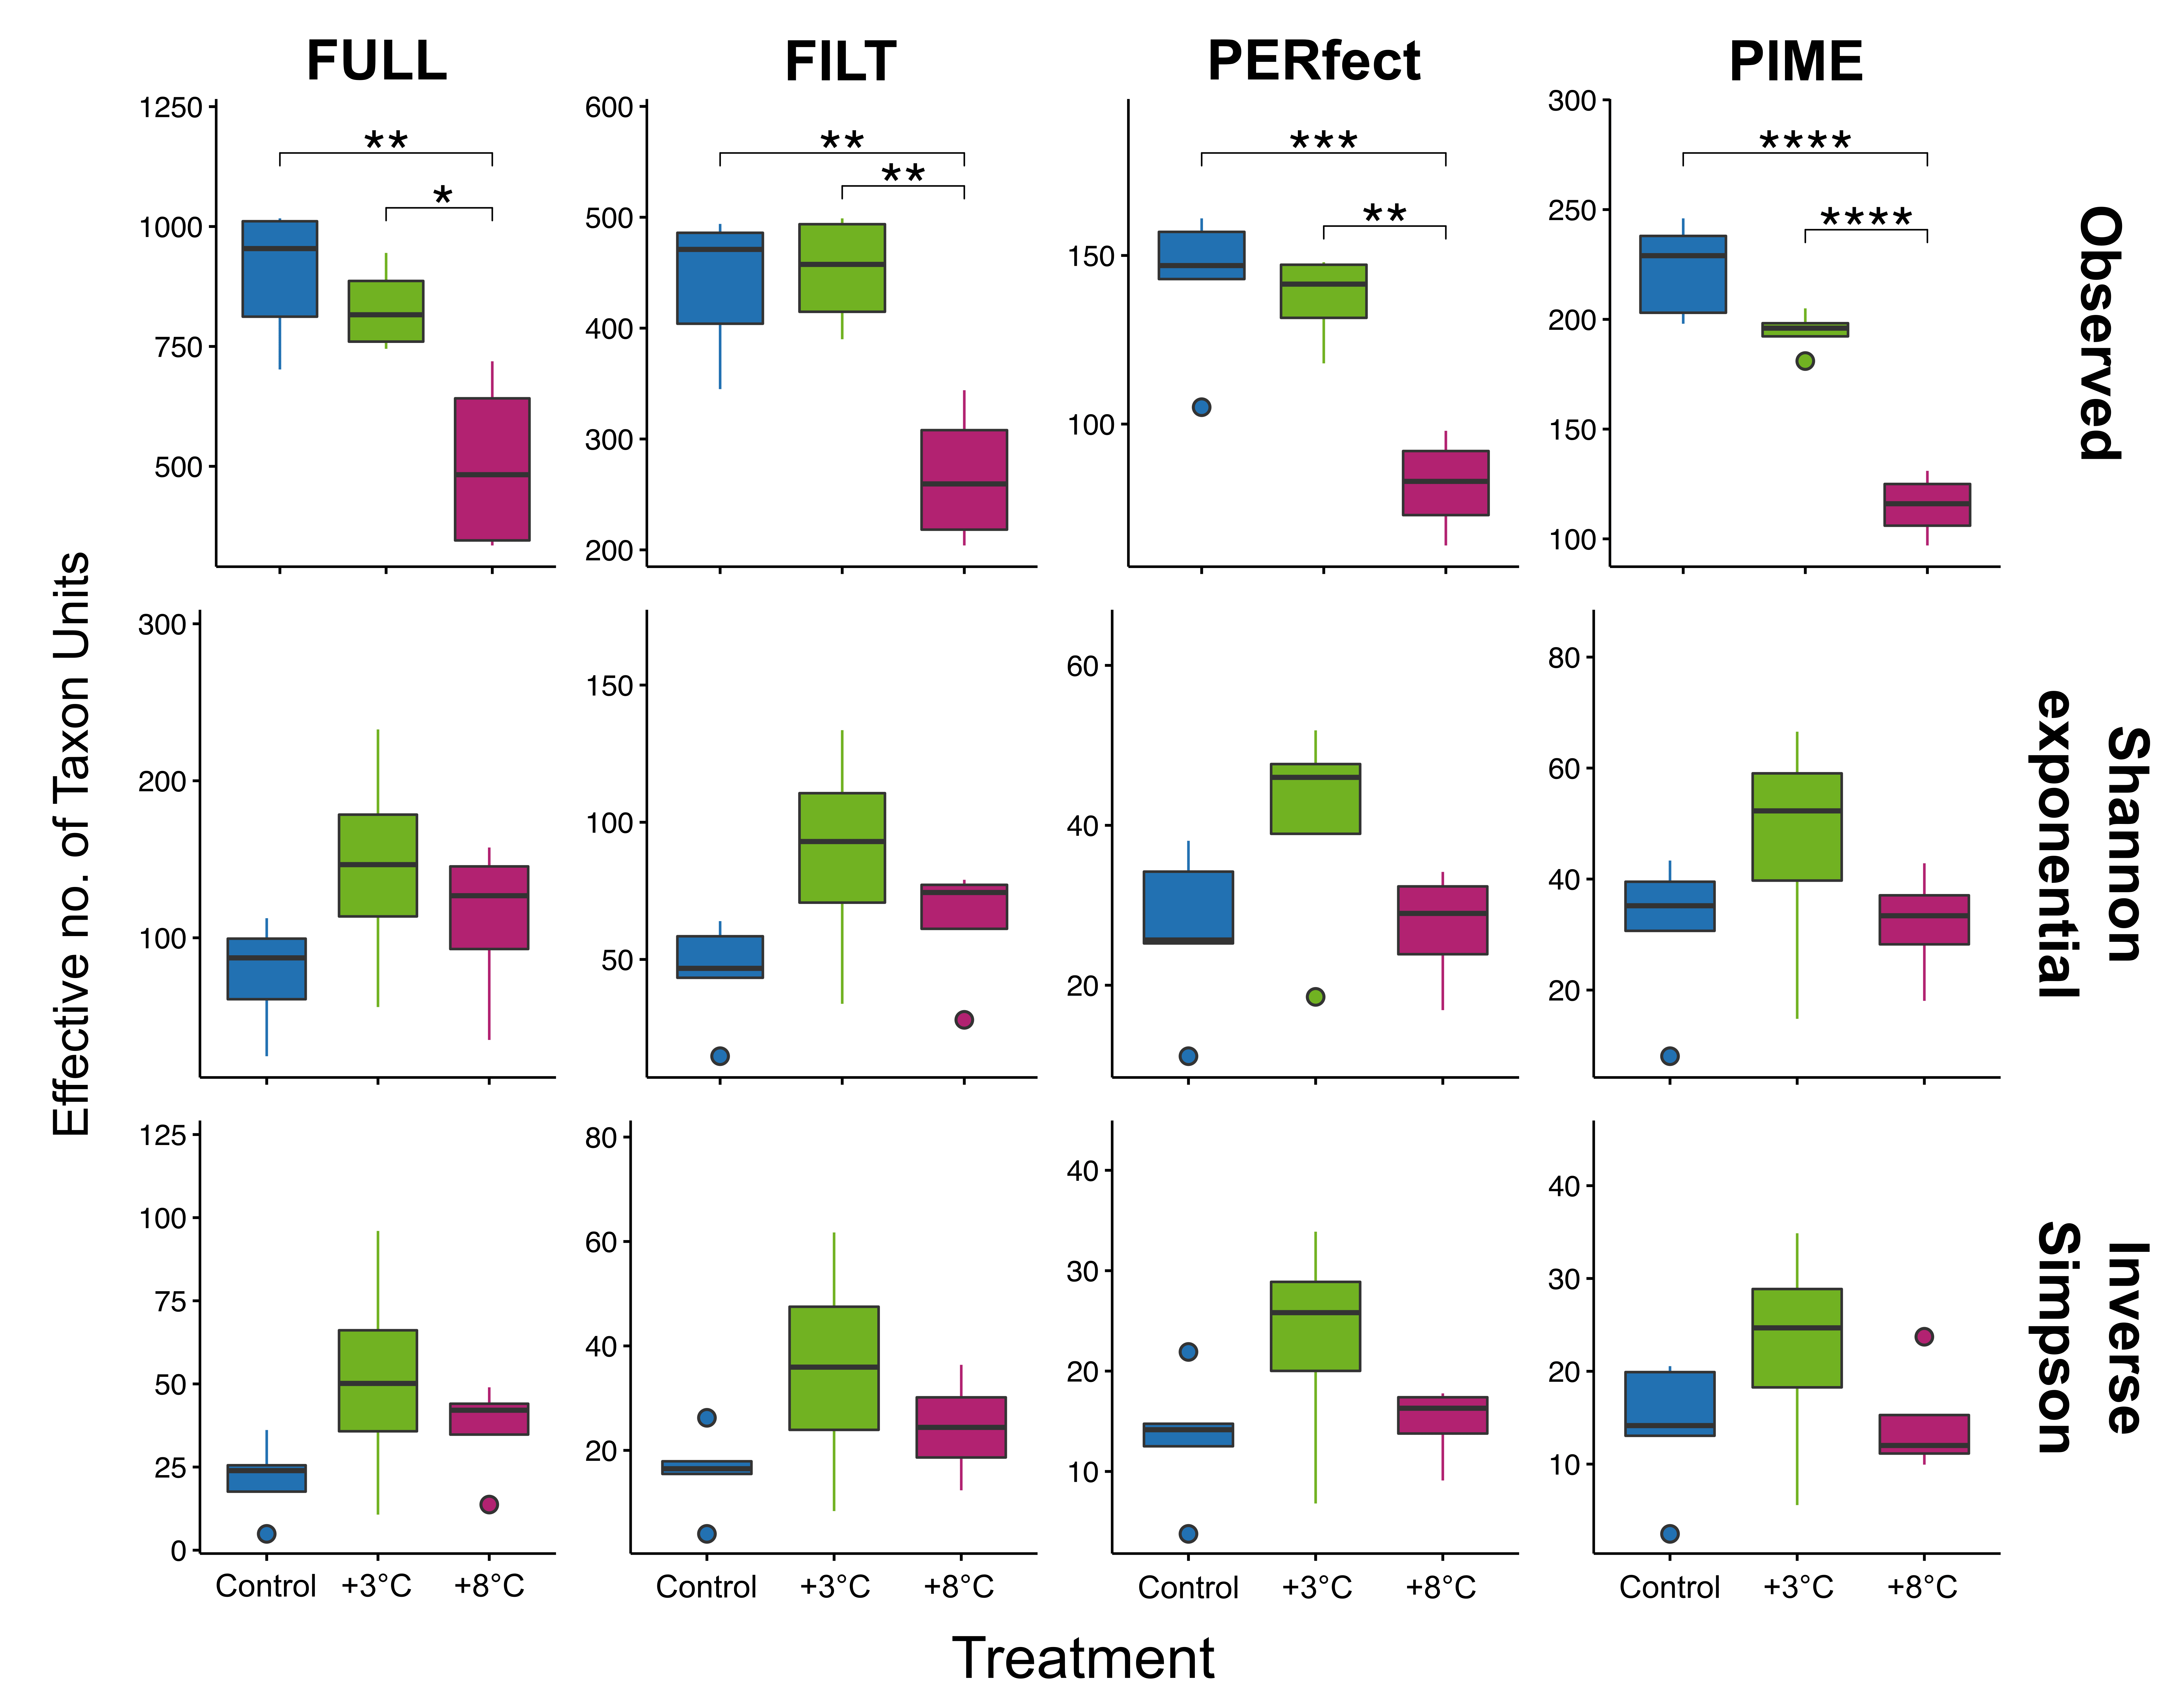
\includegraphics[width=1\textwidth,height=\textheight]{FIGURES/its_supp_alpha_div.png}

}

\caption{\textbf{Supplementary Figure 4 |} Alpha diversity estimates of
ITS communities. The centre line of each box plot represents the median,
the lower and upper hinges represent the first and third quartiles and
whiskers represent + 1.5 the interquartile range. Shapiro-Wilk Normality
Test and Bartlett Test of Homogeneity of Variances indicated all data
was normally distributed. Differences in alpha diversity for all metrics
assessed using analysis of variance (ANOVA) followed by Tukey HSD post
hoc tests. Only significant differences (p-values adjusted for multiple
comparisons) between treatments and controls are shown in plots, where n
= 5 (control) and n = 4 (treatments).}

\end{figure}

\newpage{}

\hypertarget{beta-diversity-of-microbial-communities}{%
\subsection{Beta diversity of microbial
communities}\label{beta-diversity-of-microbial-communities}}

To test for significance between treatment groups, we calculated the
beta dispersion (using the \texttt{betadisper} function, vegan package)
for each 16S rRNA distance matrix (unweighted and weighted UniFrac) and
each ITS distance matrix (Jensen-Shannon and Bray-Curtis). We then used
the function \texttt{permutest} to run a Permutation Test for
Homogeneity of multivariate dispersions against the results of each beta
dispersion test (\textbf{Supplementary Table 12}, \textbf{Supplementary
Table 13}). If the results were not significant (i.e., p-value
\textgreater{} 0.05) we ran a PERMANOVA using \texttt{adonis} (PERMANOVA
assumes equal dispersion), otherwise we used Analysis of Similarity
(ANOSIM). \textbf{Supplementary Table 14} contains the results of the
significance tests.

\begin{table}[H]

\caption{\textbf{Supplementary Table 12 |} Results of beta dispersion \& permutation test for homogeneity of multivariate dispersions (16S rRNA).}
\centering
\fontsize{8}{10}\selectfont
\begin{tabular}[t]{llcc}
\toprule
\textcolor{black}{\textbf{Description}} & \textcolor{black}{\textbf{distance metric}} & \textcolor{black}{\textbf{p-value}} & \textcolor{black}{\textbf{selected test}}\\
\midrule
\addlinespace[-0.3em]
\multicolumn{4}{l}{\textbf{}}\\
\hspace{1em}\cellcolor{gray!6}{FULL data set} & \cellcolor{gray!6}{unweighted UniFrac} & \cellcolor{gray!6}{0.013} & \cellcolor{gray!6}{ANOSIM}\\
\hspace{1em} & weighted UniFrac & 0.004 & \vphantom{1} ANOSIM\\
\addlinespace[-0.3em]
\multicolumn{4}{l}{\textbf{}}\\
\hspace{1em}\cellcolor{gray!6}{Arbitrary filter} & \cellcolor{gray!6}{unweighted UniFrac} & \cellcolor{gray!6}{0.002} & \cellcolor{gray!6}{ANOSIM}\\
\hspace{1em} & weighted UniFrac & 0.004 & ANOSIM\\
\addlinespace[-0.3em]
\multicolumn{4}{l}{\textbf{}}\\
\hspace{1em}\cellcolor{gray!6}{PERFect filter} & \cellcolor{gray!6}{unweighted UniFrac} & \cellcolor{gray!6}{0.001} & \cellcolor{gray!6}{ANOSIM}\\
\hspace{1em} & weighted UniFrac & 0.003 & ANOSIM\\
\addlinespace[-0.3em]
\multicolumn{4}{l}{\textbf{}}\\
\hspace{1em}\cellcolor{gray!6}{PIME filter} & \cellcolor{gray!6}{unweighted UniFrac} & \cellcolor{gray!6}{0.474} & \cellcolor{gray!6}{ADONIS}\\
\hspace{1em} & weighted UniFrac & 0.012 & ANOSIM\\
\bottomrule
\end{tabular}
\end{table}

\begin{table}[H]

\caption{\textbf{Supplementary Table 13 |} Results of beta dispersion \& permutation test for homogeneity of multivariate dispersions (ITS).}
\centering
\fontsize{8}{10}\selectfont
\begin{tabular}[t]{llcc}
\toprule
\textcolor{black}{\textbf{Description}} & \textcolor{black}{\textbf{distance metric}} & \textcolor{black}{\textbf{p-value}} & \textcolor{black}{\textbf{selected test}}\\
\midrule
\addlinespace[-0.3em]
\multicolumn{4}{l}{\textbf{}}\\
\hspace{1em}\cellcolor{gray!6}{FULL data set} & \cellcolor{gray!6}{Jensen-Shannon} & \cellcolor{gray!6}{0.745} & \cellcolor{gray!6}{ADONIS}\\
\hspace{1em} & Bray-Curtis & 0.696 & ADONIS\\
\addlinespace[-0.3em]
\multicolumn{4}{l}{\textbf{}}\\
\hspace{1em}\cellcolor{gray!6}{Arbitrary filter} & \cellcolor{gray!6}{Jensen-Shannon} & \cellcolor{gray!6}{0.920} & \cellcolor{gray!6}{ADONIS}\\
\hspace{1em} & Bray-Curtis & 0.864 & ADONIS\\
\addlinespace[-0.3em]
\multicolumn{4}{l}{\textbf{}}\\
\hspace{1em}\cellcolor{gray!6}{PERFect filter} & \cellcolor{gray!6}{Jensen-Shannon} & \cellcolor{gray!6}{0.865} & \cellcolor{gray!6}{ADONIS}\\
\hspace{1em} & Bray-Curtis & 0.819 & ADONIS\\
\addlinespace[-0.3em]
\multicolumn{4}{l}{\textbf{}}\\
\hspace{1em}\cellcolor{gray!6}{PIME filter} & \cellcolor{gray!6}{Jensen-Shannon} & \cellcolor{gray!6}{0.704} & \cellcolor{gray!6}{ADONIS}\\
\hspace{1em} & Bray-Curtis & 0.756 & ADONIS\\
\bottomrule
\end{tabular}
\end{table}

\begin{table}[H]

\caption{\textbf{Supplementary Table 14 |} Summary of beta diversity significant tests. Where beta dispersion tests were not significant, we used Permutational multivariate analysis of variance (PERMANOVA) to calculate dissimilarity among treatment groups. Where beta dispersion tests were significant, we used Analysis of Similarity (ANOSIM).}
\centering
\fontsize{9}{11}\selectfont
\begin{tabular}[t]{llcccc}
\toprule
\textcolor{black}{\textbf{Data set}} & \textcolor{black}{\textbf{Distance metric}} & \textcolor{black}{\textbf{(FULL)}} & \textcolor{black}{\textbf{(FILT)}} & \textcolor{black}{\textbf{(PERFect)}} & \textcolor{black}{\textbf{(PIME)}}\\
\midrule
\addlinespace[1em]
\multicolumn{6}{l}{\textbf{16S rRNA}}\\
\hspace{1em}\cellcolor{gray!6}{} & \cellcolor{gray!6}{unweighted UniFrac} & \cellcolor{gray!6}{0.003} & \cellcolor{gray!6}{0.003} & \cellcolor{gray!6}{0.003} & \cellcolor{gray!6}{0.001}\\
\hspace{1em} & weighted UniFrac & 0.001 & 0.001 & 0.001 & 0.001\\
\addlinespace[0.3em]
\multicolumn{6}{l}{\textbf{ITS}}\\
\hspace{1em}\cellcolor{gray!6}{} & \cellcolor{gray!6}{Jensen-Shannon divergence} & \cellcolor{gray!6}{0.036} & \cellcolor{gray!6}{0.030} & \cellcolor{gray!6}{0.063} & \cellcolor{gray!6}{0.002}\\
\hspace{1em} & Bray-Curtis dissimilarity & 0.047 & 0.028 & 0.079 & 0.003\\
\bottomrule
\end{tabular}
\end{table}

\hypertarget{differentially-abundant-asvs}{%
\subsection{Differentially abundant
ASVs}\label{differentially-abundant-asvs}}

Indicator Species Analysis (ISA) of the 16S rRNA data set identified 251
differentially abundant (DA) ASVs. Of those, 154 ASVs were enriched in
the Control samples, 82 in the +3°C treatment, and 15 in the +8°C
treatment (\textbf{Supplementary Dataset4}). Linear discriminant
analysis (LDA) effect size (LEfSe) identified 676 DA ASVs with an LDA
score \textgreater{} 2.0 and a p-value \textless{} 0.05. Of those, 355
ASVs were enriched in the Control samples, 227 in the +3°C treatment,
and 94 in the +8°C treatment (\textbf{Supplementary Dataset5}).

ISA of the ITS data set identified 203 DA ASVs. Of those, 54 ASVs were
enriched in the Control samples, 95 in the +3°C treatment, and 54 in the
+8°C treatment (\textbf{Supplementary Dataset6}). LEfSe identified 228
DA ASVs with an LDA score \textgreater{} 2.0 and a p-value \textless{}
0.05. Of those, 52 ASVs were enriched in the Control samples, 107 in the
+3°C treatment, and 69 in the +8°C treatment (\textbf{Supplementary
Dataset7}).

\hypertarget{multivariate-analysis-1}{%
\subsection{Multivariate analysis}\label{multivariate-analysis-1}}

\hypertarget{normality-tests-parameter-normalization}{%
\subsubsection{Normality tests \& parameter
normalization}\label{normality-tests-parameter-normalization}}

We used Shapiro-Wilk Normality Test\textsuperscript{18} to determine
which of the 61 metadata parameters were or were not normally
distributed. For the 16S rRNA data we needed to transform 25 metadata
parameters (p-value \textless{} 0.05) and for the ITS data, 21 metadata
parameters needed transformation (p-value \textless{} 0.05). Please see
the project website for the specific parameters that were transformed
and the method of transformation used in each case
(\url{https://sweltr.github.io/high-temp/metadata.html}). For both
community data sets, \texttt{bestNormalize} was unable to find a
suitable transformation for \texttt{Al} and \texttt{Fe.} This is likely
because there was very little variation in these parameters and/or there
were too few significant digits.

\hypertarget{removing-autocorrelated-parameters}{%
\subsubsection{Removing autocorrelated
parameters}\label{removing-autocorrelated-parameters}}

Based on autocorrelation tests between the metadata and community data
(\textbf{Supplementary Figure 5, Supplementary Figure 6}), we removed
the following parameters:

Environmental and edaphic properties: TEB, DON, Na, Al, Ca.\\
Microbial functional responses: micN, micNP, enzCN, enzCP,
BP\textsubscript{ase}, CE\textsubscript{ase}, LP\textsubscript{ase},
N\textsubscript{ase}, P\textsubscript{ase}.\\
Temperature adaptation: NUE, PUE, SI.

We removed P\textsubscript{Q10} (temperature adaptation) from the ITS
analysis based on the autocorrelation tests.

\begin{figure}

{\centering 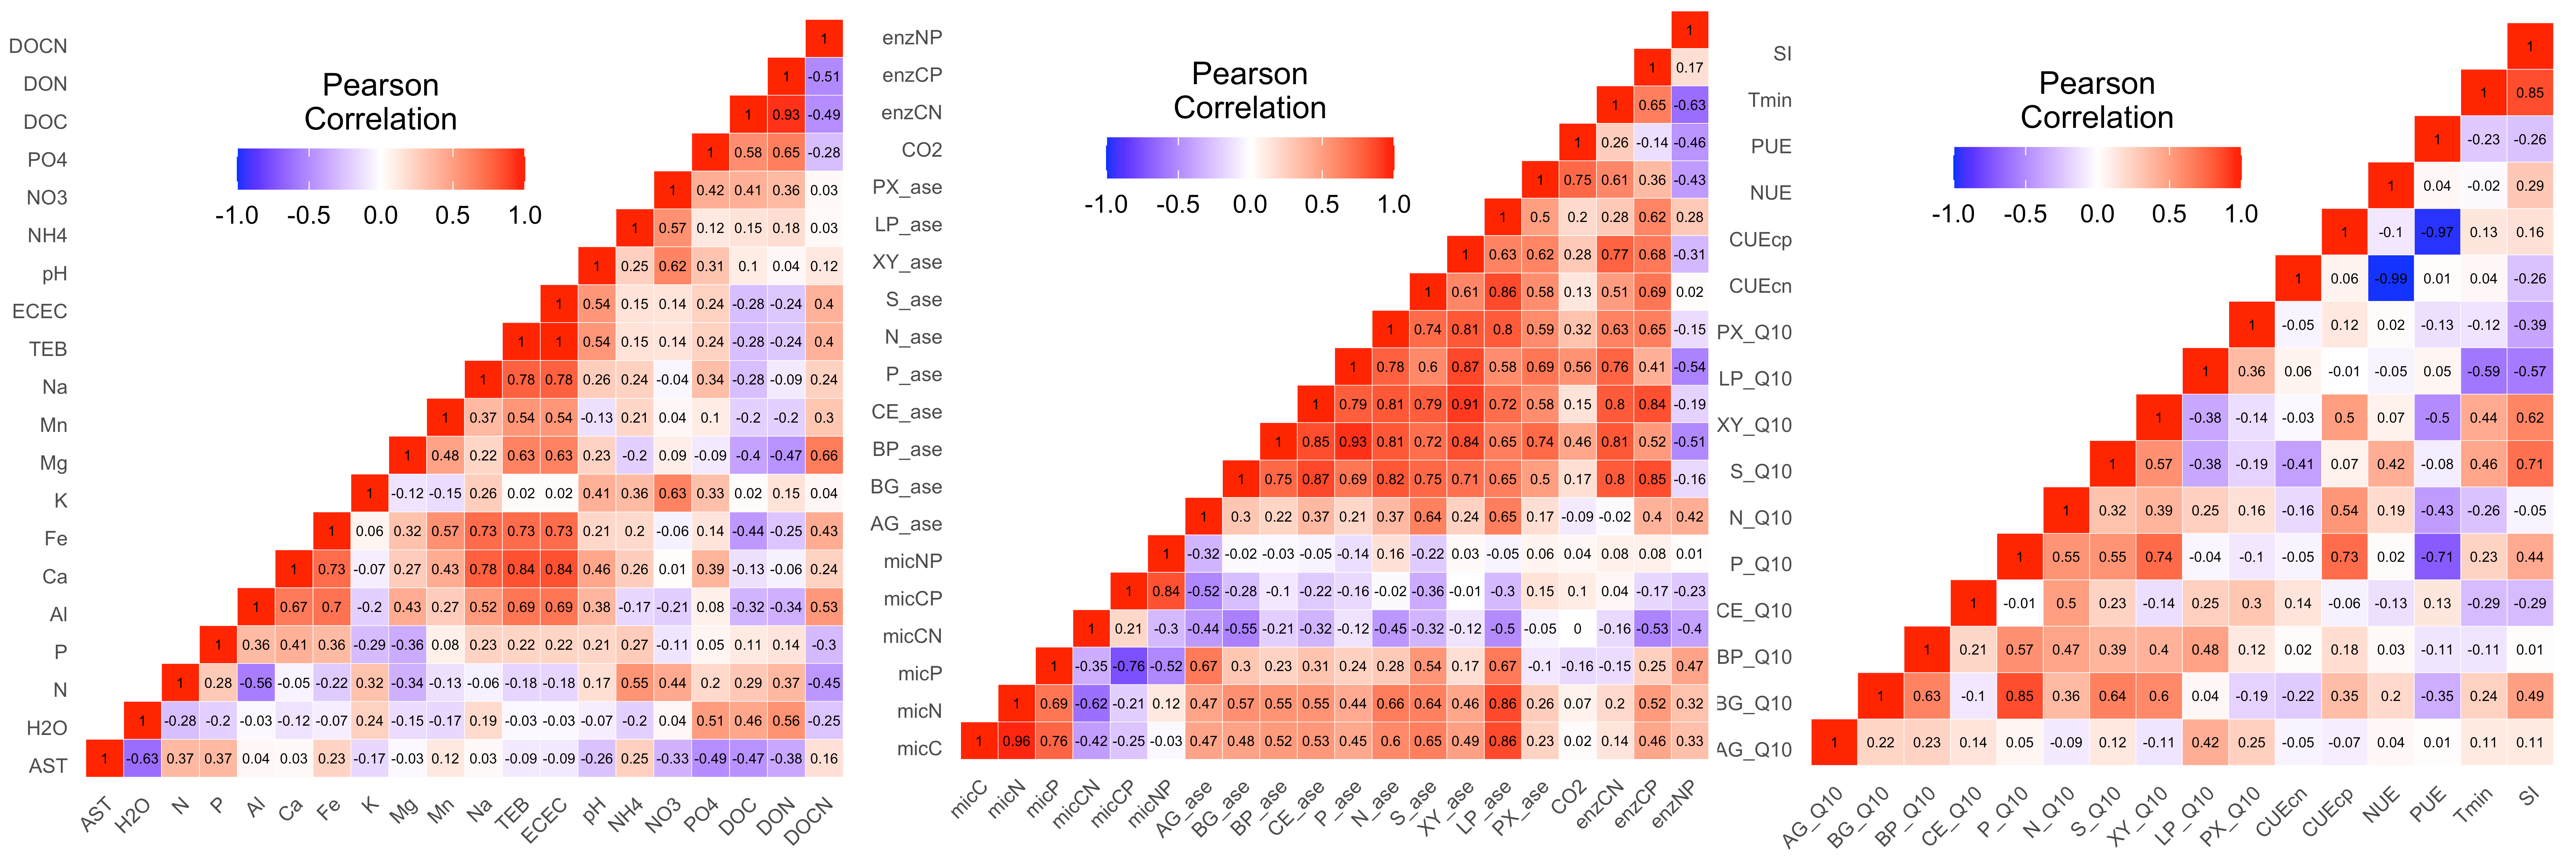
\includegraphics[width=1\textwidth,height=\textheight]{FIGURES/ssu18_auto_cor_combo.png}

}

\caption{\textbf{Supplementary Figure 5 |} Autocorrelation plots (16S
rRNA) against: (left) environmental \& edaphic properties; (middle)
microbial functional responses; \& (right) temperature adaptation.}

\end{figure}

\begin{figure}

{\centering 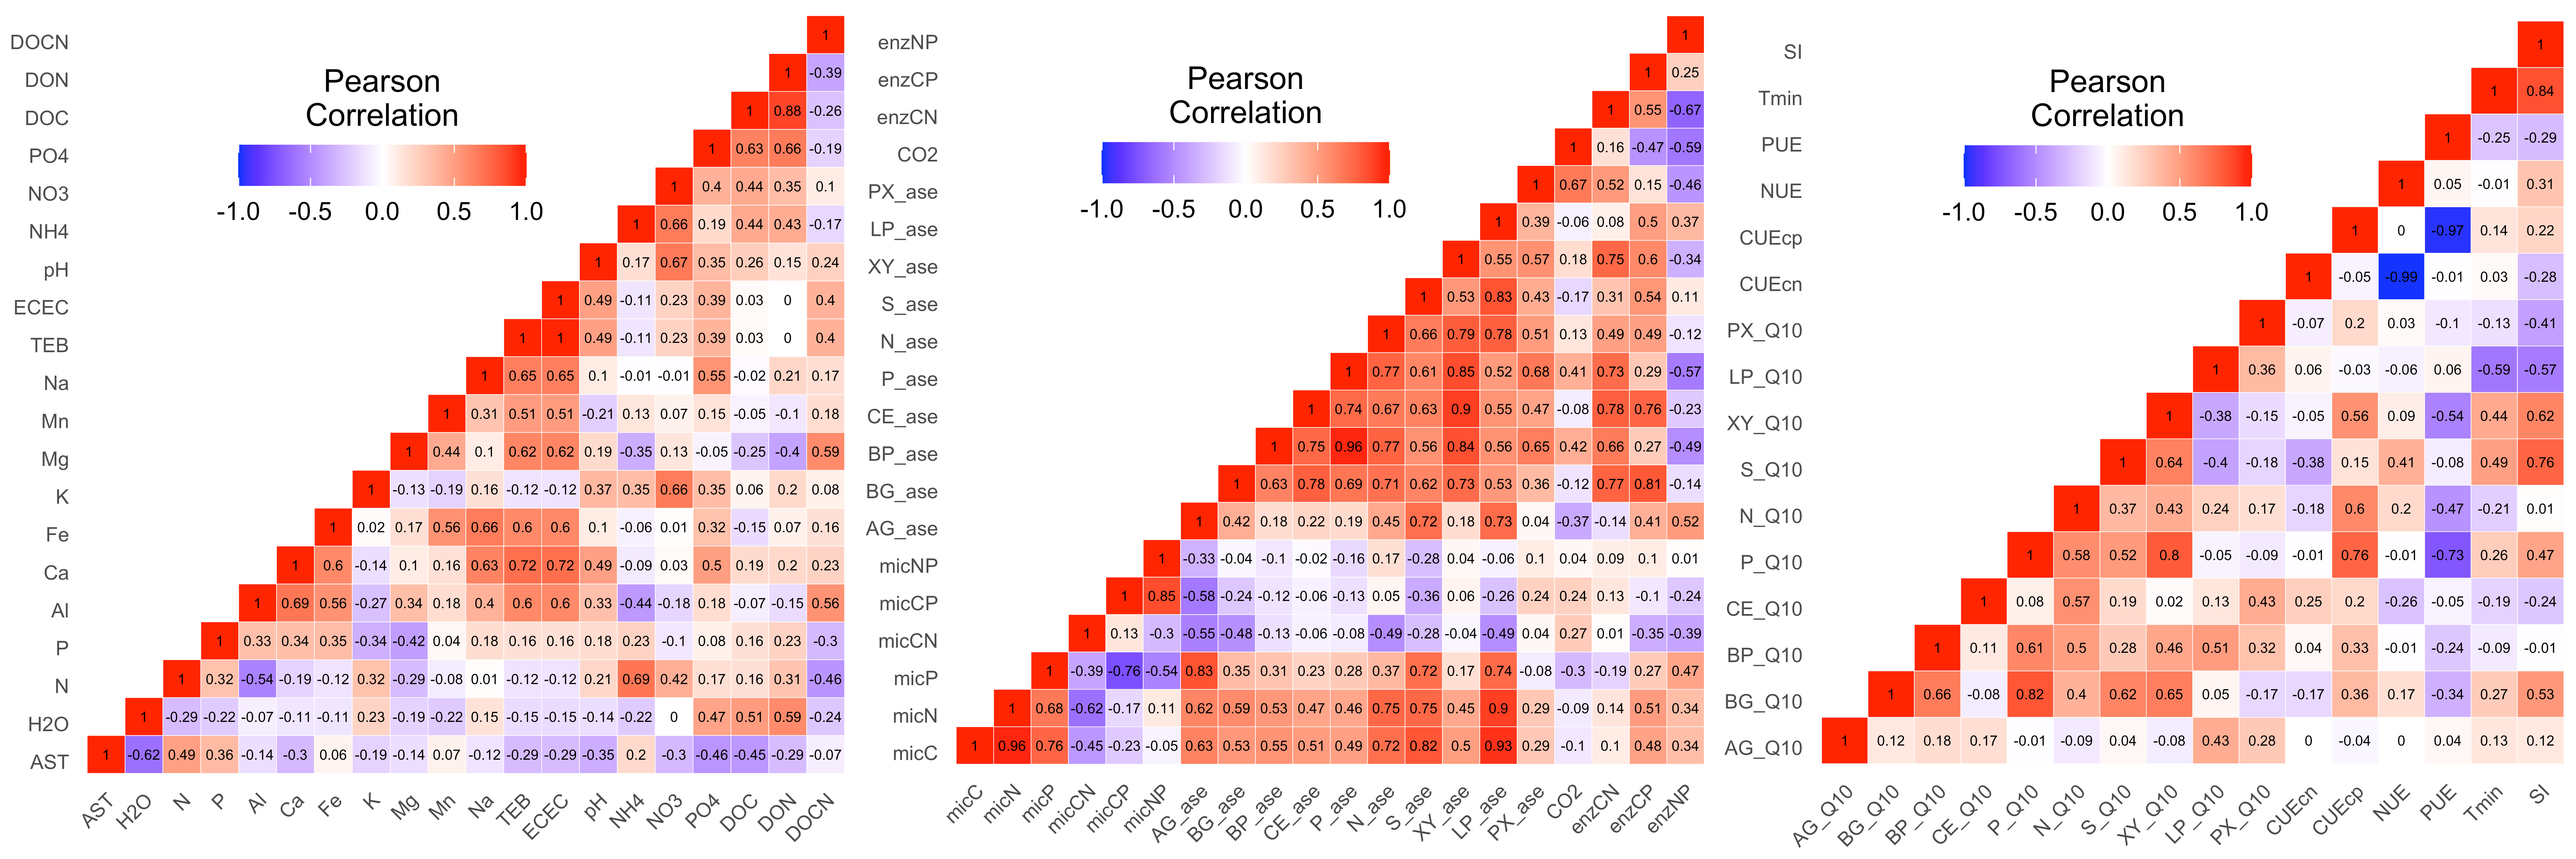
\includegraphics[width=1\textwidth,height=\textheight]{FIGURES/its18_auto_cor_combo.png}

}

\caption{\textbf{Supplementary Figure 6 |} Autocorrelation plots (ITS)
against: (left) environmental \& edaphic properties; (middle) microbial
functional responses; \& (right) temperature adaptation.}

\end{figure}

\hypertarget{dissimilarity-correlation-tests}{%
\subsubsection{Dissimilarity correlation
tests}\label{dissimilarity-correlation-tests}}

We used Mantel Tests to determine if any metadata groups were
significantly correlated with 16S rRNA or ITS community data
(\textbf{Supplementary Table 15}).

\begin{table}[H]

\caption{\textbf{Supplementary Table 15 |} Mantel tests for 16S rRNA \& ITS data compared to each of the three metadata groups. Significant differences denoted by p-values < 0.05.}
\centering
\fontsize{9}{11}\selectfont
\begin{tabular}[t]{lccc}
\toprule
\textcolor{black}{\textbf{Data set}} & \textcolor{black}{\textbf{edaphic properties}} & \textcolor{black}{\textbf{soil functional response}} & \textcolor{black}{\textbf{temperature adaptation}}\\
\midrule
\cellcolor{gray!6}{16S rRNA} & \cellcolor{gray!6}{0.003} & \cellcolor{gray!6}{0.180} & \cellcolor{gray!6}{0.001}\\
ITS & 0.002 & 0.288 & 0.001\\
\bottomrule
\end{tabular}
\end{table}

\hypertarget{best-subset-of-variables}{%
\subsubsection{Best subset of
variables}\label{best-subset-of-variables}}

The \texttt{bioenv} function found the following metadata parameters
(normalized with autocorrelated data removed) significantly correlated
with community data (results of Mantel tests shown in parentheses).

\underline{Environmental and edaphic properties}

\textbf{16S rRNA}: AST (\emph{r} = 1.0, \emph{p} = 0.001).\\
\textbf{ITS}: AST (\emph{r} = 1.0, \emph{p} = 0.001).

\underline{Microbial functional responses}

\textbf{16S rRNA}: AG\textsubscript{ase} (\emph{r} = 0.559, \emph{p} =
0.001), enzNP (\emph{r} = 0.462, \emph{p} = 0.006), S\textsubscript{ase}
(\emph{r} = 0.614, \emph{p} = 0.001), PX\textsubscript{ase} (\emph{r} =
0.612, \emph{p} = 0.001), XY\textsubscript{ase} (\emph{r} = 0.456,
\emph{p} = 0.002).\\
\textbf{ITS}: enzNP (\emph{r} = 0.553, \emph{p} = 0.001),
PX\textsubscript{ase} (\emph{r} = 0.685, \emph{p} = 0.001),
XY\textsubscript{ase} (\emph{r} = 0.505, \emph{p} = 0.002).

\underline{Temperature adaptation}

\textbf{16S rRNA}: CUE\textsubscript{cp} (\emph{r} = 0.325, \emph{p} =
0.013), LP\textsubscript{Q10} (\emph{r} = 0.377, \emph{p} = 0.005),
P\textsubscript{Q10} (\emph{r} = 0.518, \emph{p} = 0.001),
S\textsubscript{Q10} (\emph{r} = 0.440, \emph{p} = 0.001), and
T\textsubscript{min} (\emph{r} = 0.404, \emph{p} = 0.005).\\
\textbf{ITS}: XY\textsubscript{Q10} (\emph{r} = 0.726, \emph{p} =
0.001), T\textsubscript{min} (\emph{r} = 0.616, \emph{p} = 0.001).

\hypertarget{distance-based-redundancy-analysis-dbrda}{%
\subsubsection{Distance-based Redundancy Analysis
(dbRDA)}\label{distance-based-redundancy-analysis-dbrda}}

In all cases (i.e., both community data sets against each of the three
metadata subsets), \texttt{rankindex}\textsuperscript{35} indicated that
Bray-Curtis was best dissimilarity metric to use. Based on these
results, we set \texttt{dist\ =\ "bray"} for each dbRDA analysis using
\texttt{capscale}. Due to issue pertaining to degrees of freedom, we
needed to remove some metadata parameters from specific groups. From the
16S rRNA analysis, we removed Mg and Mn (environmental and edaphic
properties). From the ITS analysis, we removed Mg, Mn, Na, Al, Fe, and K
(environmental and edaphic properties) and S\textsubscript{Q10}
(temperature adaptation). Next, we used the vegan function
\texttt{envfit} to fit environmental parameters onto the ordination.
This function calculates correlation scores between metadata parameters
and ordination axes. \texttt{envfit} found the following parameters were
significantly correlated with community data (Goodness of fit
statistic/squared correlation coefficient and empirical p-values for
each variable shown in parentheses).

\underline{Environmental and edaphic properties}

\textbf{16S rRNA}: AST (\emph{r\textsuperscript{2}} =0.829, \emph{p} =
0.001), H\textsubscript{2}O (\emph{r\textsuperscript{2}} =0.519,
\emph{p} = 0.010), DOC (\emph{r\textsuperscript{2}} =0.446, \emph{p} =
0.024).\\
\textbf{ITS}: AST (\emph{r\textsuperscript{2}} =0.485, \emph{p} =
0.037), DOC (\emph{r\textsuperscript{2}} =0.535, \emph{p} = 0.028).

\underline{Microbial functional responses}

\textbf{16S rRNA}: AG\textsubscript{ase} (\emph{r\textsuperscript{2}} =
0.444, \emph{p} = 0.026), BG\textsubscript{ase}
(\emph{r\textsuperscript{2}} = 0.560, \emph{p} = 0.007),
S\textsubscript{ase} (\emph{r\textsuperscript{2}} = 0.737, \emph{p} =
0.002), XY\textsubscript{ase} (\emph{r\textsuperscript{2}} = 0.519,
\emph{p} = 0.009), PX\textsubscript{ase} (\emph{r\textsuperscript{2}} =
0.764, \emph{p} = 0.001), CO\textsubscript{2}
(\emph{r\textsuperscript{2}} = 0.504, \emph{p} = 0.013), enzNP
(\emph{r\textsuperscript{2}} = 0.624, \emph{p} = 0.004).\\
\textbf{ITS}: micP (\emph{r\textsuperscript{2}} = 0.693, \emph{p} =
0.002), micCP (\emph{r\textsuperscript{2}} = 0.583, \emph{p} = 0.016),
AG\textsubscript{ase} (\emph{r\textsuperscript{2}} = 0.506, \emph{p} =
0.037), PX\textsubscript{ase} (\emph{r\textsuperscript{2}} = 0.500,
\emph{p} = 0.035), enzNP (\emph{r\textsuperscript{2}} = 0.547, \emph{p}
= 0.014).

\underline{Temperature adaptation}

\textbf{16S rRNA}: S\textsubscript{Q10} (\emph{r\textsuperscript{2}} =
0.496, \emph{p} = 0.015), XY\textsubscript{Q10}
(\emph{r\textsuperscript{2}} = 0.373, \emph{p} = 0.049),
LP\textsubscript{Q10} (\emph{r\textsuperscript{2}} = 0.413, \emph{p} =
0.041), T\textsubscript{min} (\emph{r\textsuperscript{2}} = 0.446,
\emph{p} = 0.030).\\
\textbf{ITS}: XY\textsubscript{Q10} (\emph{r\textsuperscript{2}} =
0.617, \emph{p} = 0.010), CUE\textsubscript{cp}
(\emph{r\textsuperscript{2}} = 0.479, \emph{p} = 0.035),
T\textsubscript{min} (\emph{r\textsuperscript{2}} = 0.475, \emph{p} =
0.028).

\newpage{}

\hypertarget{appendices}{%
\section{Appendices}\label{appendices}}

\hypertarget{appendix-1}{%
\subsection{Appendix 1: Description of Supplementary
Datasets}\label{appendix-1}}

For this study, \textbf{Supplementary Datasets} are text files that were
too large to include in the Supplementary Material. The individual files
can be downloaded from the journal's website. Below are descriptions for
each Supplementary Data item.

\hypertarget{supplementary-dataset1}{%
\subsubsection{Supplementary Dataset1}\label{supplementary-dataset1}}

\textbf{Description:} Output from the \textbf{16S rRNA} DADA2 workflow
before manual curation. Table is a tab delimited text file containing
information for 20,332 ASVs. The first column is the unique ASV ID,
followed by the read counts for each sample, ASV taxonomic lineage
(Kingdom to Genus), and finally the unique ASV sequence.

\begin{tcolorbox}[enhanced jigsaw, opacityback=0, left=2mm, breakable, bottomrule=.15mm, colframe=quarto-callout-note-color-frame, colback=white, leftrule=.75mm, toprule=.15mm, arc=.35mm, rightrule=.15mm]
\textbf{Filename} Supplementary\_Dataset1.txt
\end{tcolorbox}

\hypertarget{supplementary-dataset2}{%
\subsubsection{Supplementary Dataset2}\label{supplementary-dataset2}}

\textbf{Description:} Output from the \textbf{ITS} DADA2 workflow before
manual curation. Table is a tab delimited text file containing
information for 3357 ASVs. The first column is the unique ASV ID,
followed by the read counts for each sample, ASV taxonomic lineage
(Kingdom to Genus), and finally the unique ASV sequence.

\begin{tcolorbox}[enhanced jigsaw, opacityback=0, left=2mm, breakable, bottomrule=.15mm, colframe=quarto-callout-note-color-frame, colback=white, leftrule=.75mm, toprule=.15mm, arc=.35mm, rightrule=.15mm]
\textbf{Filename} Supplementary\_Dataset2.txt
\end{tcolorbox}

\hypertarget{supplementary-dataset3}{%
\subsubsection{Supplementary Dataset3}\label{supplementary-dataset3}}

\textbf{Description:} Complete \textbf{metadata} information collected
in this study. Tab delimited text file containing data for 61 metadata
parameters (before normalization) associated with each sample. The first
column is the sample ID, followed plot number (1--10), treatment
(control or warm), temperature (0°C, +3°C, +8°C), plot pair ID (A--E),
and collection season (W = rainy season). Subsequent columns contain
values for all metadata parameters.

\begin{tcolorbox}[enhanced jigsaw, opacityback=0, left=2mm, breakable, bottomrule=.15mm, colframe=quarto-callout-note-color-frame, colback=white, leftrule=.75mm, toprule=.15mm, arc=.35mm, rightrule=.15mm]
\textbf{Filename} Supplementary\_Dataset3.txt
\end{tcolorbox}

\hypertarget{supplementary-dataset4}{%
\subsubsection{Supplementary Dataset4}\label{supplementary-dataset4}}

\textbf{Description:} Differentially abundant (DA) ASVs from the
\textbf{16S rRNA} data identified using Indicator Species Analysis (ISA)
against the PIME filtered data set. Tab delimited text file of all 251
DA ASVs between temperature treatments.

\begin{tcolorbox}[enhanced jigsaw, opacityback=0, left=2mm, breakable, bottomrule=.15mm, colframe=quarto-callout-note-color-frame, colback=white, leftrule=.75mm, toprule=.15mm, arc=.35mm, rightrule=.15mm]
\textbf{Filename} Supplementary\_Dataset4.txt
\end{tcolorbox}

Description of table headers:

\begin{itemize}
\tightlist
\item
  \textbf{ASV\_ID} ASV name.
\item
  \textbf{group} Sample group ASV is enriched in.
\item
  \textbf{indval} Indicator value from Dufrene-Legendre Indicator
  Species Analysis.
\item
  \textbf{pval} p-value from Dufrene-Legendre Indicator Species
  Analysis.
\item
  \textbf{freq} Total number of samples where ASV was detected.
\item
  \textbf{freq\_C0} Total number of Control samples where ASV was
  detected.
\item
  \textbf{freq\_W3} Total number of +3°C samples where ASV was detected.
\item
  \textbf{freq\_W8} Total number of +8°C samples where ASV was detected.
\item
  \textbf{reads\_total} Total reads in data set.
\item
  \textbf{reads\_C0} Total reads in Control samples.
\item
  \textbf{reads\_W3} Total reads in +3°C samples.
\item
  \textbf{reads\_W8} Total reads in +8°C samples.
\end{itemize}

The remaining columns contain lineage information for each ASV followed
by its' unique sequence.

\hypertarget{supplementary-dataset5}{%
\subsubsection{Supplementary Dataset5}\label{supplementary-dataset5}}

\textbf{Description:} Differentially abundant (DA) ASVs from the
\textbf{16S rRNA} data identified using linear discriminant analysis
(LDA) effect size (LEfSe) against the PIME filtered data set. Tab
delimited text file of all 676 DA ASVs between temperature treatments.

\begin{tcolorbox}[enhanced jigsaw, opacityback=0, left=2mm, breakable, bottomrule=.15mm, colframe=quarto-callout-note-color-frame, colback=white, leftrule=.75mm, toprule=.15mm, arc=.35mm, rightrule=.15mm]
\textbf{Filename} Supplementary\_Dataset5.txt
\end{tcolorbox}

Description of table headers:

\begin{itemize}
\tightlist
\item
  \textbf{ASV\_ID} ASV name.
\item
  \textbf{group} Sample group ASV is enriched in.
\item
  \textbf{lda} Linear discriminant analysis (LDA) scores.
\item
  \textbf{pval} p-value from LEfSe analysis.
\item
  \textbf{freq} Total number of samples where ASV was detected.
\item
  \textbf{freq\_C0} Total number of Control samples where ASV was
  detected.
\item
  \textbf{freq\_W3} Total number of +3°C samples where ASV was detected.
\item
  \textbf{freq\_W8} Total number of +8°C samples where ASV was detected.
\item
  \textbf{reads\_total} Total reads in data set.
\item
  \textbf{reads\_C0} Total reads in Control samples.
\item
  \textbf{reads\_W3} Total reads in +3°C samples.
\item
  \textbf{reads\_W8} Total reads in +8°C samples.
\end{itemize}

The remaining columns contain lineage information for each ASV followed
by its' unique sequence.

\hypertarget{supplementary-dataset6}{%
\subsubsection{Supplementary Dataset6}\label{supplementary-dataset6}}

\textbf{Description:} Differentially abundant (DA) ASVs from the
\textbf{ITS} data identified using Indicator Species Analysis (ISA)
against the PIME filtered data set. Tab delimited text file of all 203
DA ASVs between temperature treatments.

\begin{tcolorbox}[enhanced jigsaw, opacityback=0, left=2mm, breakable, bottomrule=.15mm, colframe=quarto-callout-note-color-frame, colback=white, leftrule=.75mm, toprule=.15mm, arc=.35mm, rightrule=.15mm]
\textbf{Filename} Supplementary\_Dataset6.txt
\end{tcolorbox}

Description of table headers:

\begin{itemize}
\tightlist
\item
  \textbf{ASV\_ID} ASV name.
\item
  \textbf{group} Sample group ASV is enriched in.
\item
  \textbf{indval} Indicator value from Dufrene-Legendre Indicator
  Species Analysis.
\item
  \textbf{pval} p-value from Dufrene-Legendre Indicator Species
  Analysis.
\item
  \textbf{freq} Total number of samples where ASV was detected.
\item
  \textbf{freq\_C0} Total number of Control samples where ASV was
  detected.
\item
  \textbf{freq\_W3} Total number of +3°C samples where ASV was detected.
\item
  \textbf{freq\_W8} Total number of +8°C samples where ASV was detected.
\item
  \textbf{reads\_total} Total reads in data set.
\item
  \textbf{reads\_C0} Total reads in Control samples.
\item
  \textbf{reads\_W3} Total reads in +3°C samples.
\item
  \textbf{reads\_W8} Total reads in +8°C samples.
\end{itemize}

The remaining columns contain lineage information for each ASV followed
by its' unique sequence.

\hypertarget{supplementary-dataset7}{%
\subsubsection{Supplementary Dataset7}\label{supplementary-dataset7}}

\textbf{Description:} Differentially abundant (DA) ASVs from the
\textbf{ITS} data identified using linear discriminant analysis (LDA)
effect size (LEfSe) against the PIME filtered data set. Tab delimited
text file of all 228 DA ASVs between temperature treatments.

\begin{tcolorbox}[enhanced jigsaw, opacityback=0, left=2mm, breakable, bottomrule=.15mm, colframe=quarto-callout-note-color-frame, colback=white, leftrule=.75mm, toprule=.15mm, arc=.35mm, rightrule=.15mm]
\textbf{Filename} Supplementary\_Dataset7.txt
\end{tcolorbox}

Description of table headers:

\begin{itemize}
\tightlist
\item
  \textbf{ASV\_ID} ASV name.
\item
  \textbf{group} Sample group ASV is enriched in.
\item
  \textbf{lda} Linear discriminant analysis (LDA) scores.
\item
  \textbf{pval} p-value from LEfSe analysis.
\item
  \textbf{freq} Total number of samples where ASV was detected.
\item
  \textbf{freq\_C0} Total number of Control samples where ASV was
  detected.
\item
  \textbf{freq\_W3} Total number of +3°C samples where ASV was detected.
\item
  \textbf{freq\_W8} Total number of +8°C samples where ASV was detected.
\item
  \textbf{reads\_total} Total reads in data set.
\item
  \textbf{reads\_C0} Total reads in Control samples.
\item
  \textbf{reads\_W3} Total reads in +3°C samples.
\item
  \textbf{reads\_W8} Total reads in +8°C samples.
\end{itemize}

The remaining columns contain lineage information for each ASV followed
by its' unique sequence.

\newpage{}

\hypertarget{appendix-2}{%
\subsection{Appendix 2: Family-level bacterial
charts}\label{appendix-2}}

Top twelve (12) families of abundant bacterial phyla. Remaining taxa are
grouped in \emph{Other}. In cases where ASVs could not be classified to
family level, abundance data was calculated for the next highest
taxonomic rank, denoted by the prefix \textbf{rank abbreviation} plus
\textbf{underscore} (e.g., \textbf{c\_} is Class). As above, relative
abundance of taxa based on the full, unfiltered data set. Left plots
show taxa collapsed by temperature treatment while right plots show
individual samples faceted by temperature treatment. Taxa are ordered
first by rank and then alphabetically. The same color palette displayed
in the same order was used for each plot.

\begin{figure}

{\centering 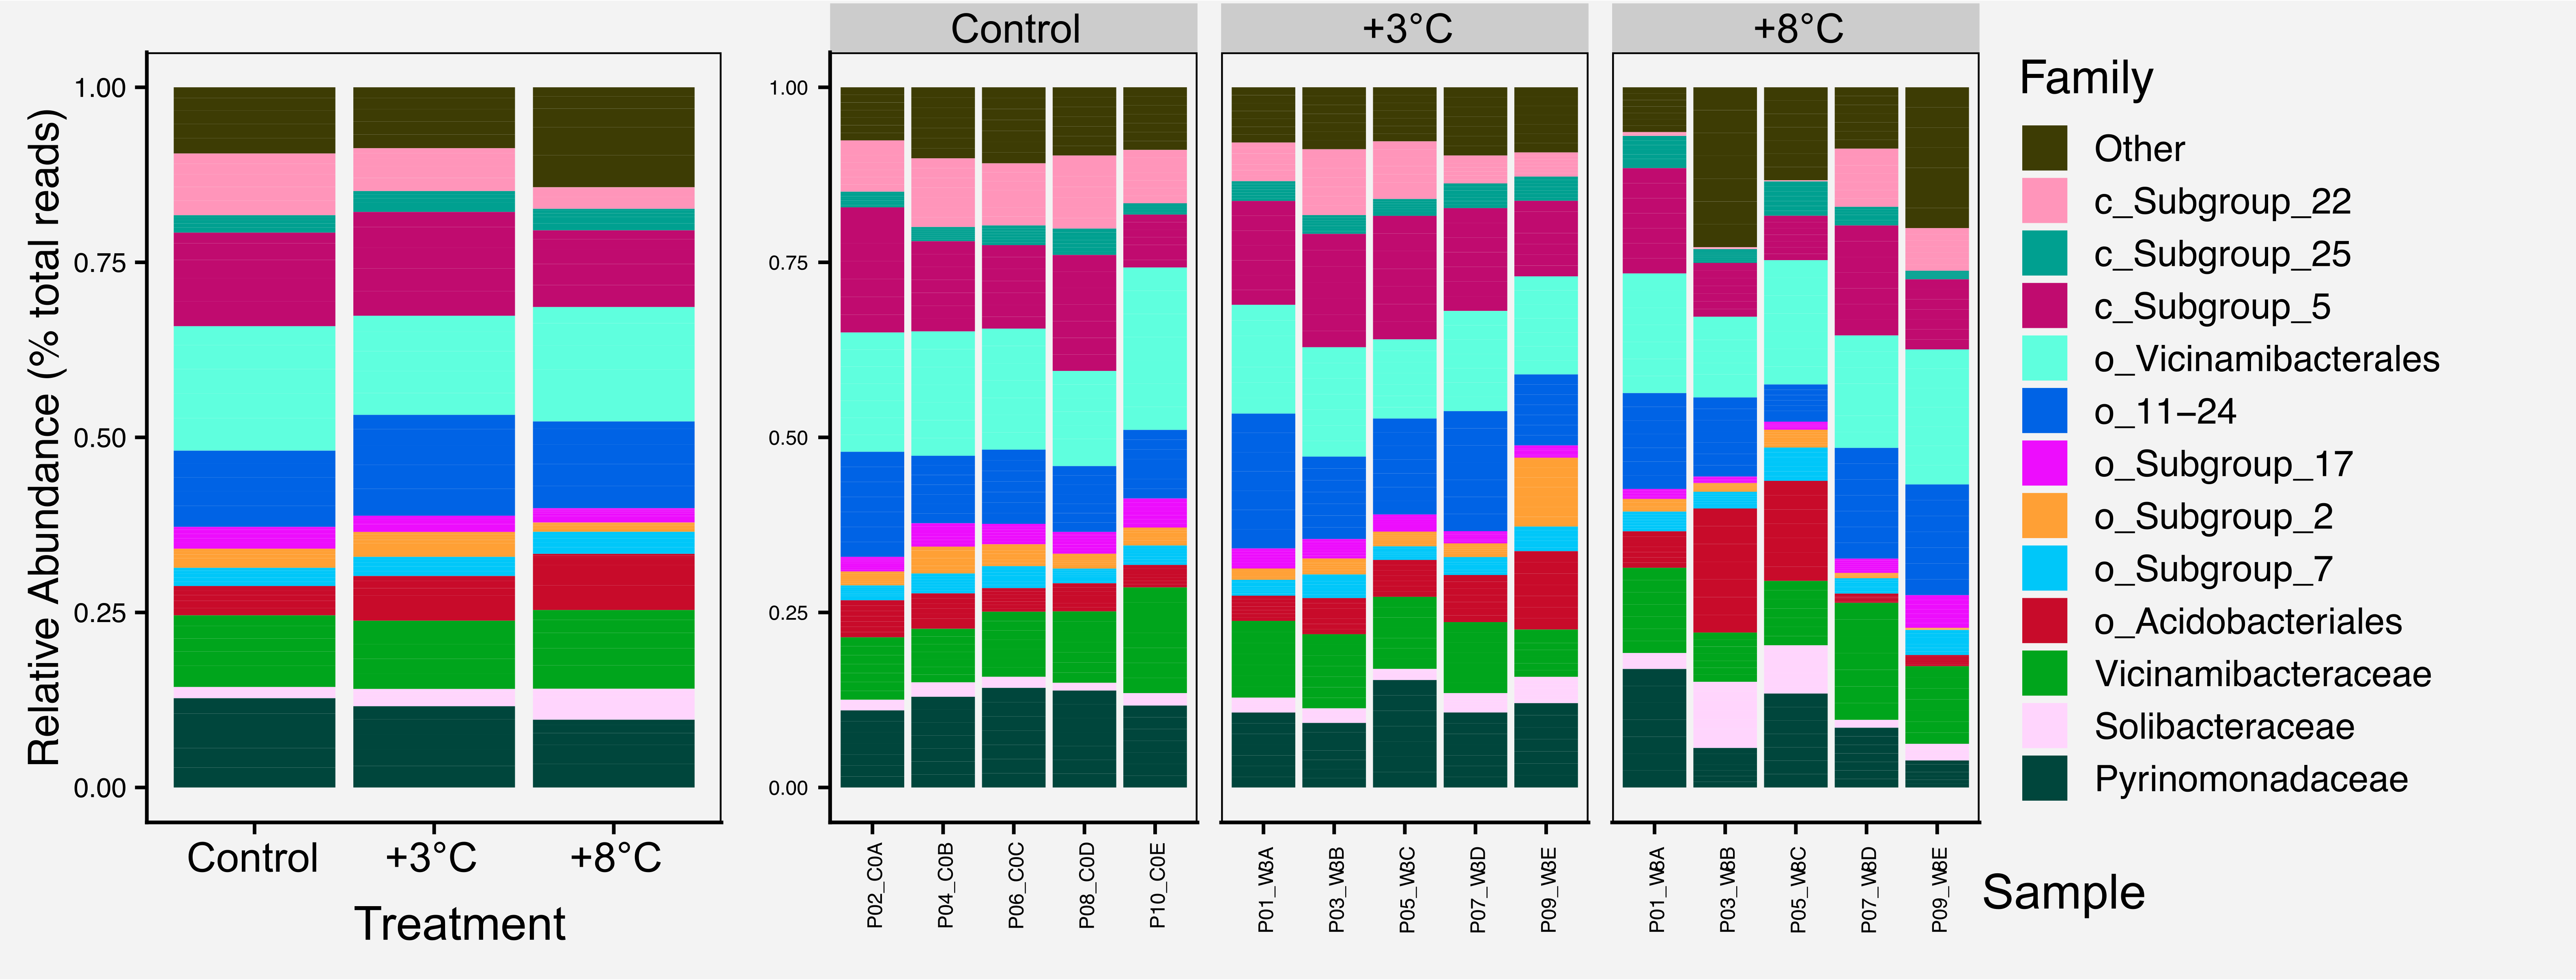
\includegraphics[width=0.95\textwidth,height=\textheight]{FIGURES/taxa_plots_class_Acido.png}

}

\caption{\textbf{Supplementary Figure 7 |} Acidobacteriota family
plots.}

\end{figure}

\begin{figure}

{\centering 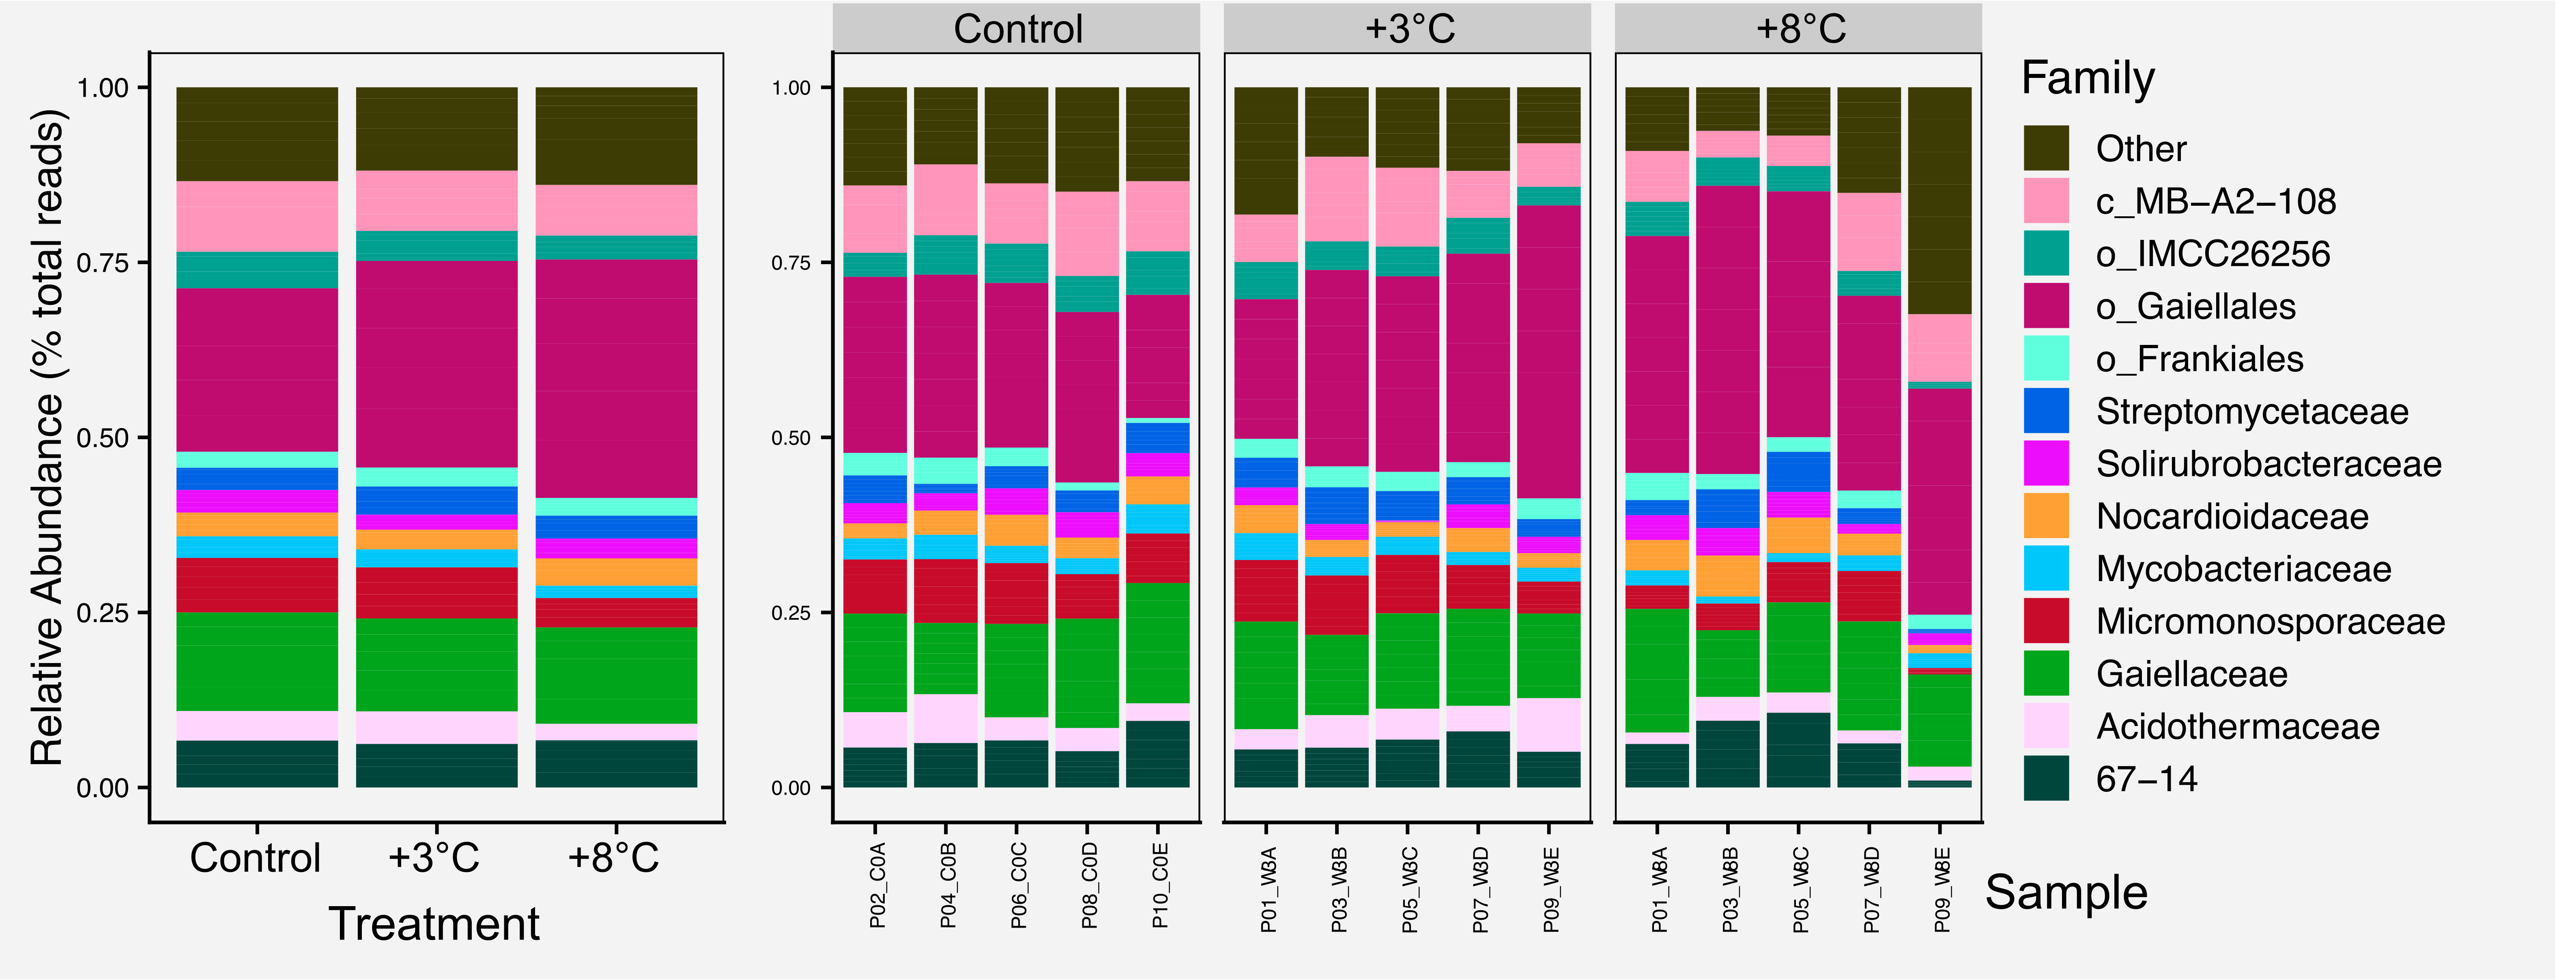
\includegraphics[width=0.95\textwidth,height=\textheight]{FIGURES/taxa_plots_class_Actino.png}

}

\caption{\textbf{Supplementary Figure 8 |} Actinobacteriota family
plots.}

\end{figure}

\begin{figure}

{\centering 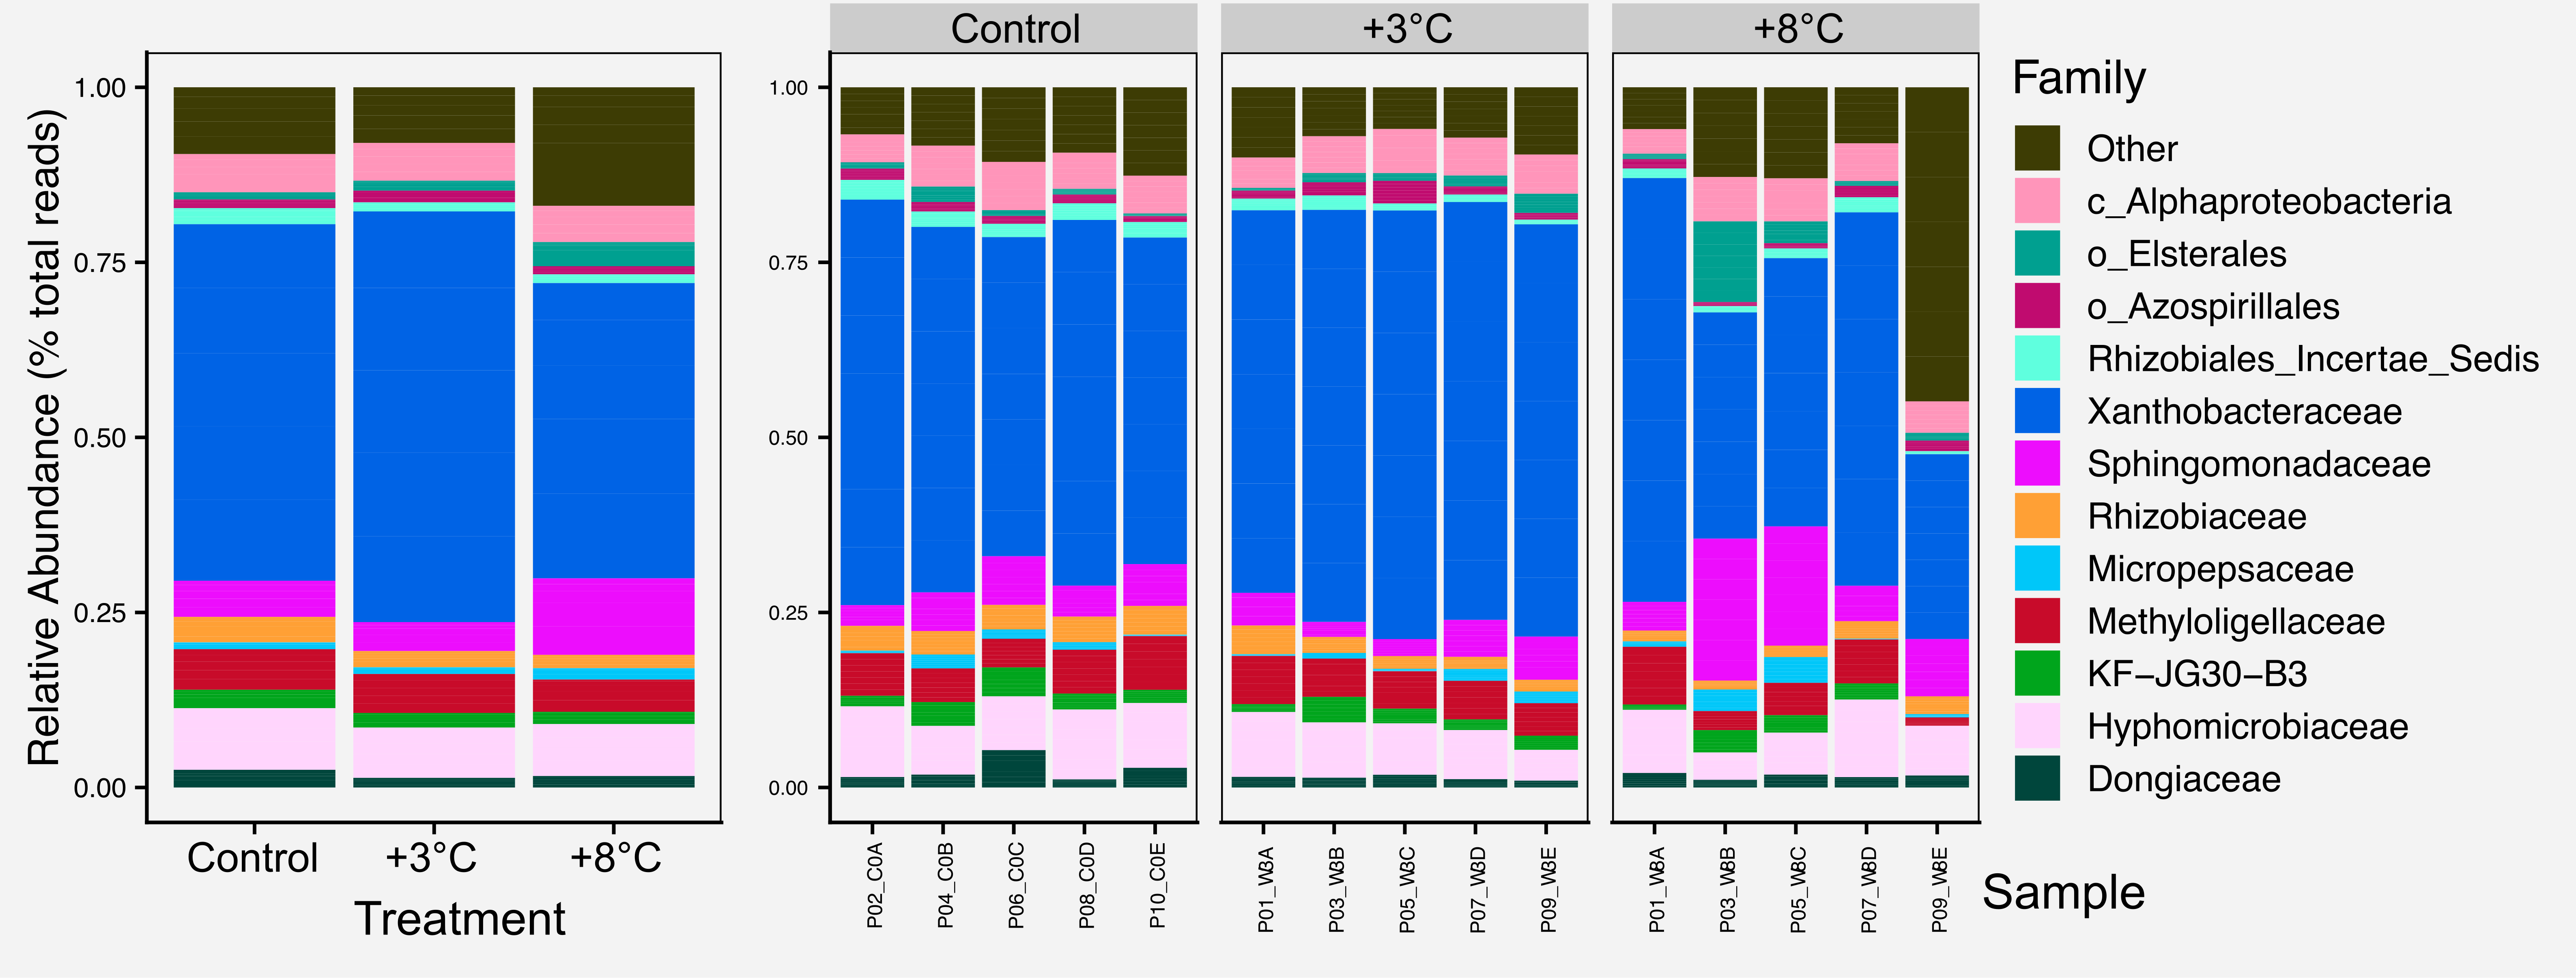
\includegraphics[width=0.95\textwidth,height=\textheight]{FIGURES/taxa_plots_class_Alpha.png}

}

\caption{\textbf{Supplementary Figure 9 |} Alphaproteobacteria family
plots.}

\end{figure}

\begin{figure}

{\centering 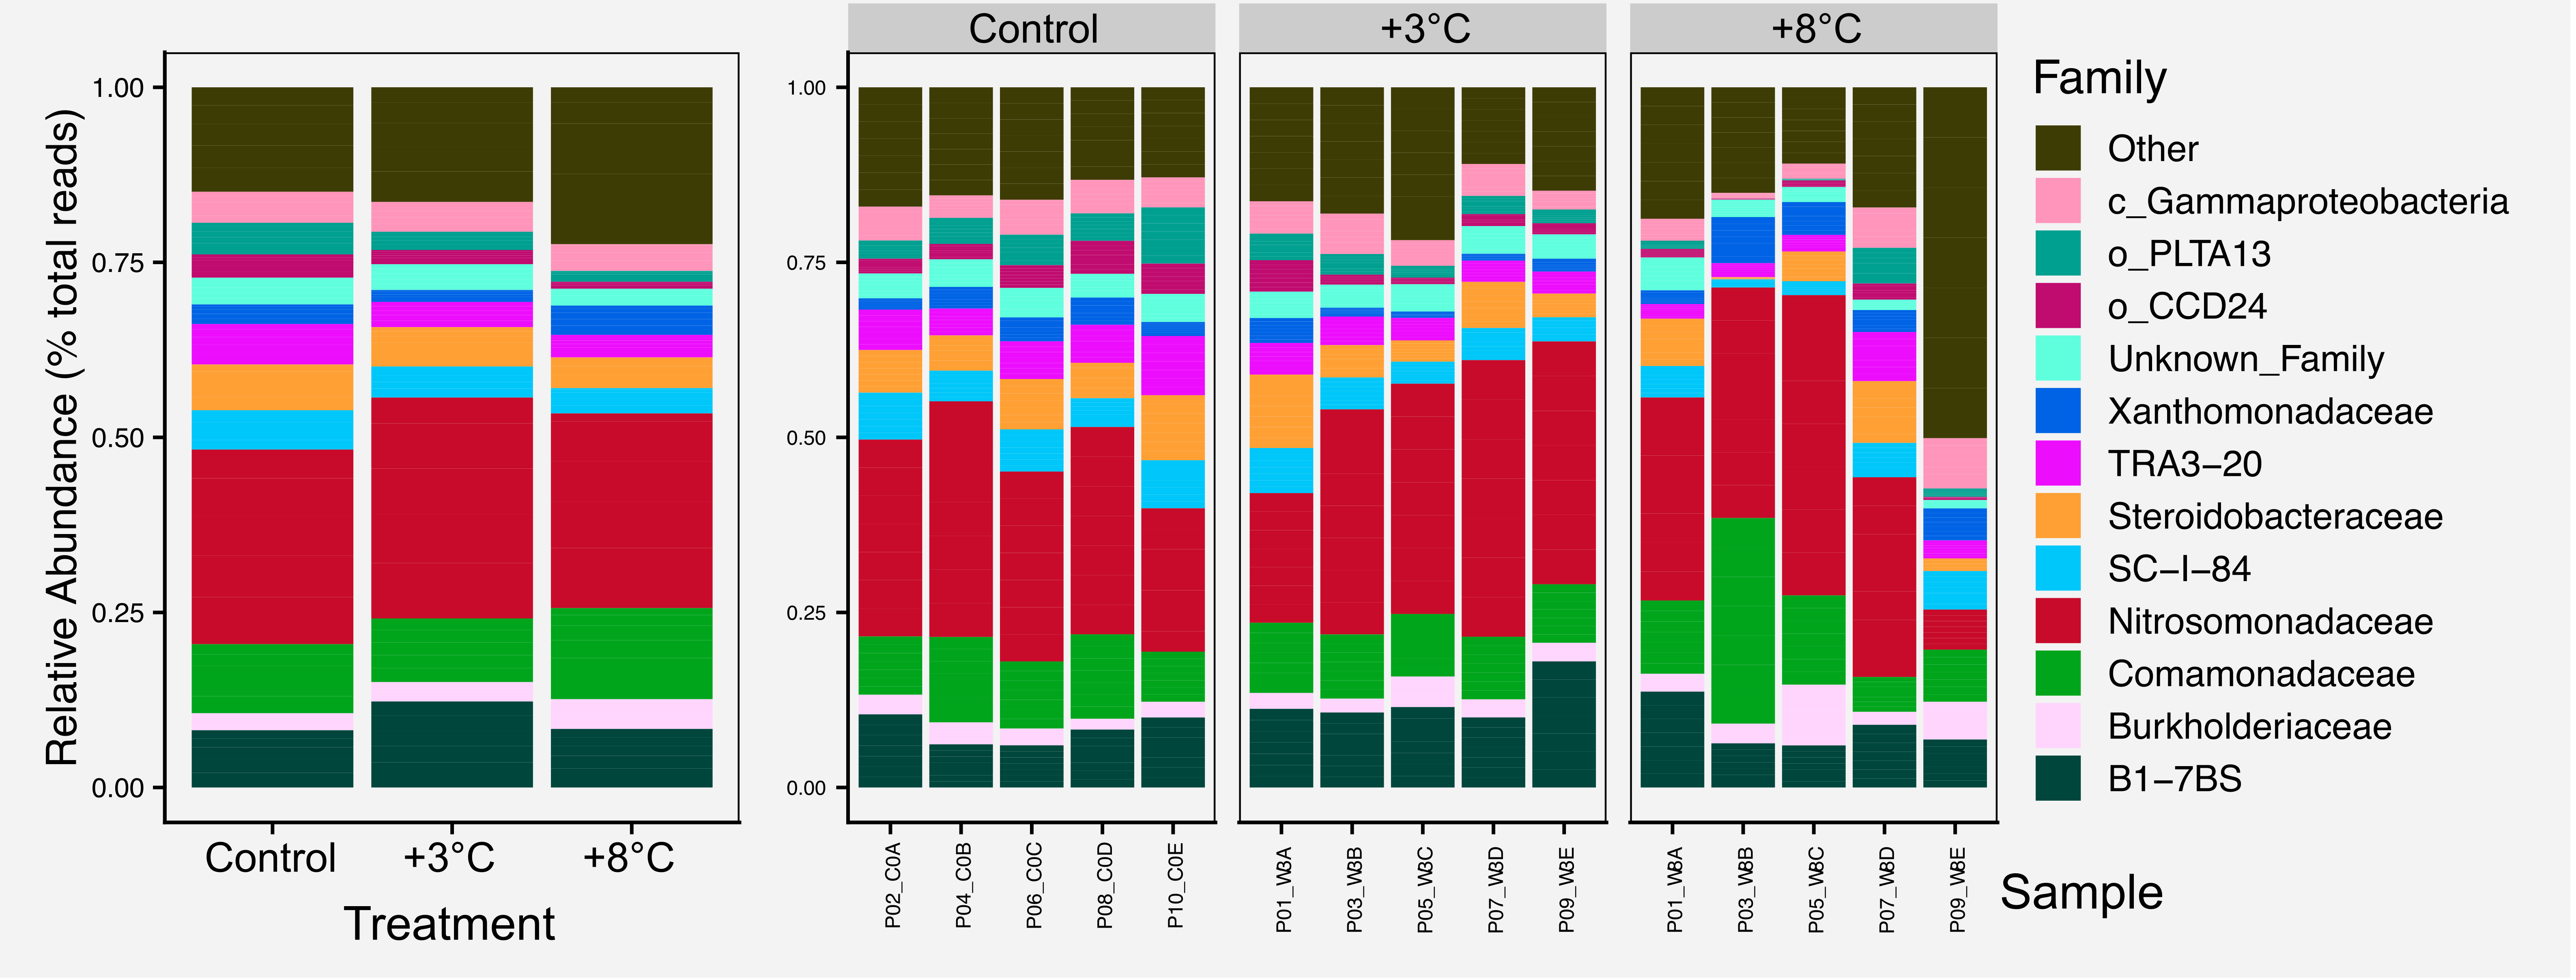
\includegraphics[width=0.95\textwidth,height=\textheight]{FIGURES/taxa_plots_class_Gamma.png}

}

\caption{\textbf{Supplementary Figure 10 |} Gammaproteobacteria family
plots.}

\end{figure}

\begin{figure}

{\centering 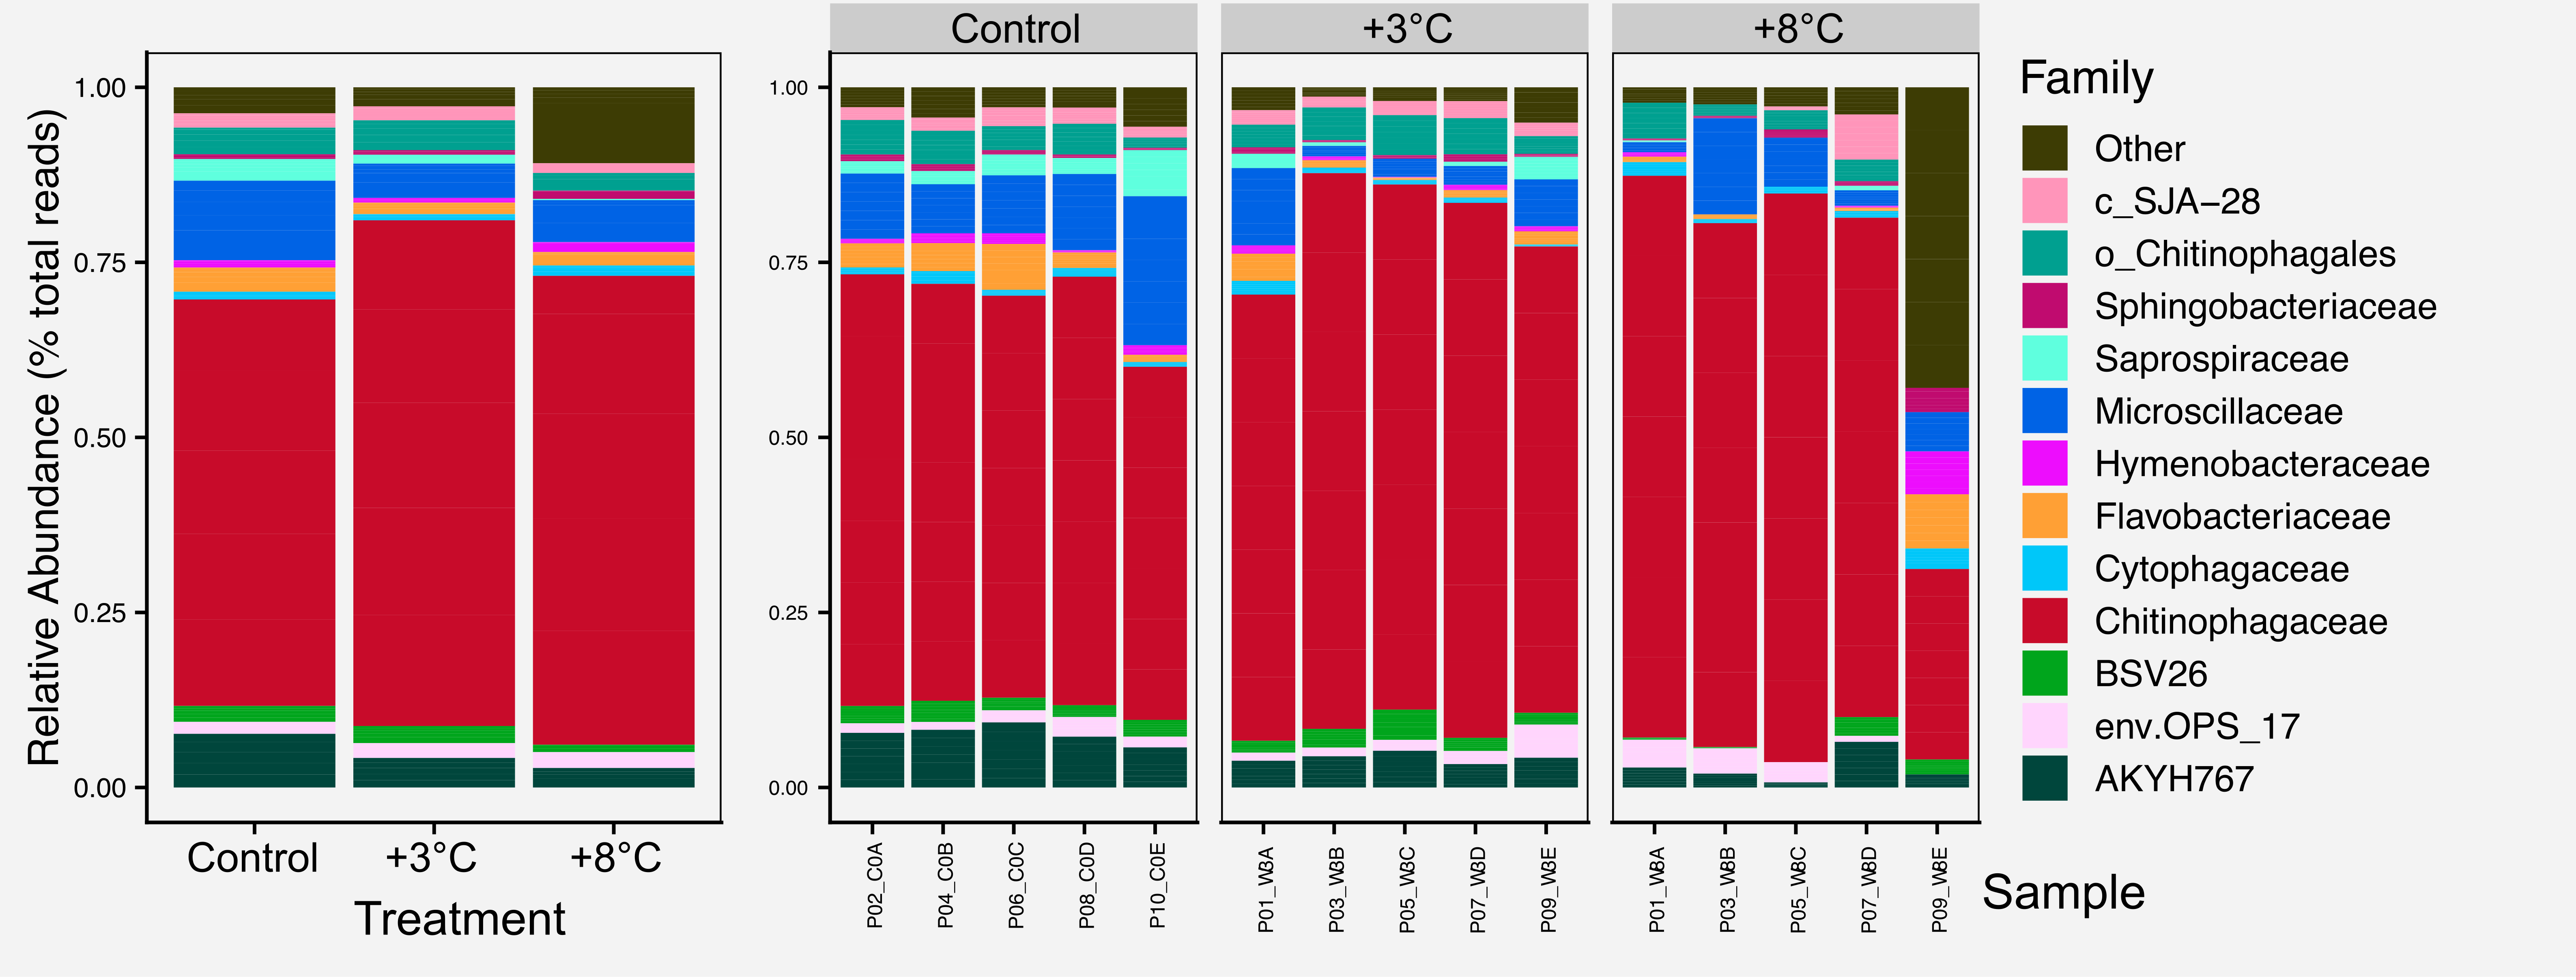
\includegraphics[width=0.95\textwidth,height=\textheight]{FIGURES/taxa_plots_class_Bacter.png}

}

\caption{\textbf{Supplementary Figure 11 |} Bacteroidota family plots.}

\end{figure}

\begin{figure}

{\centering 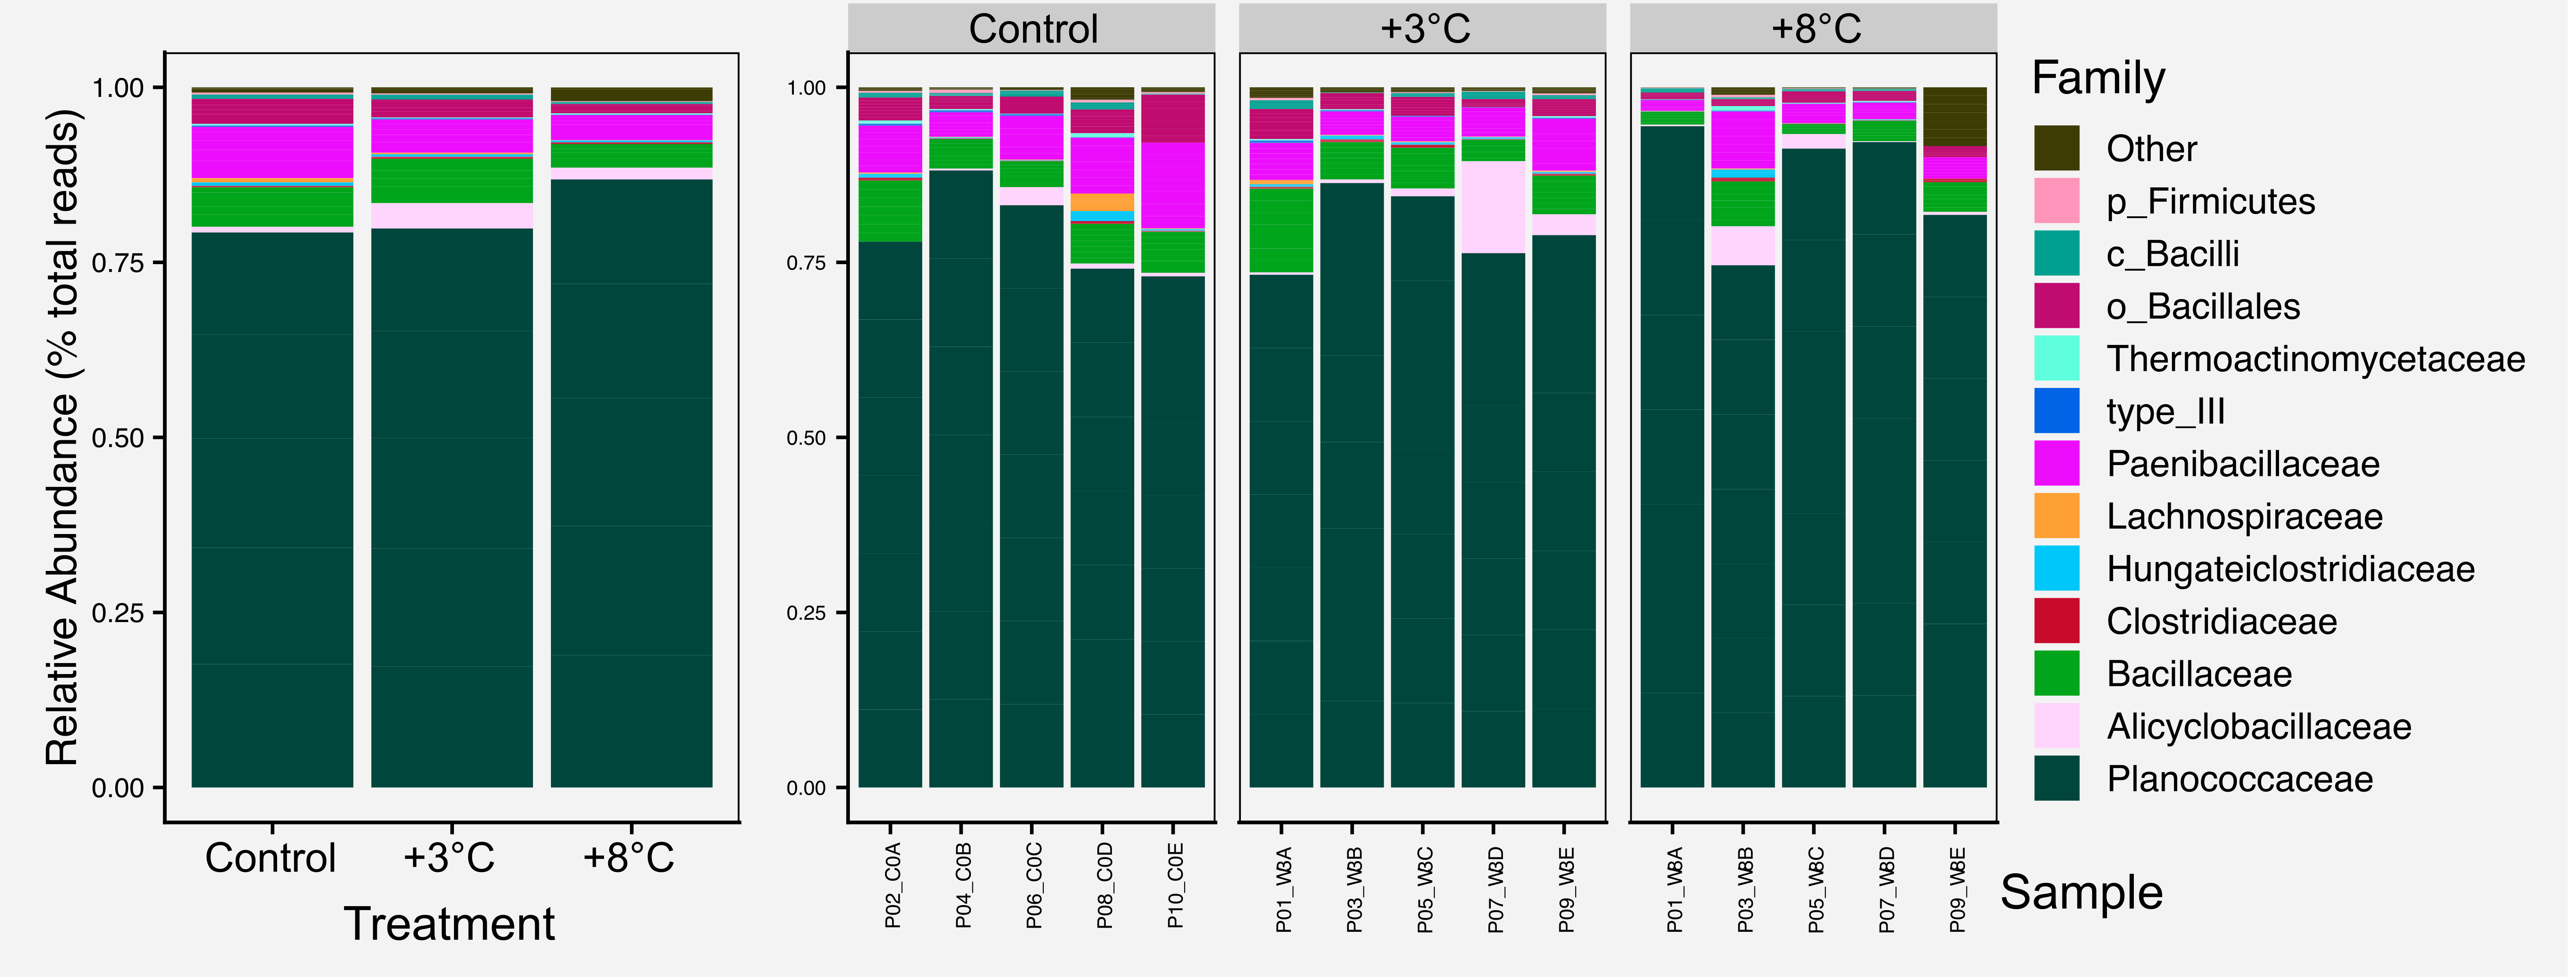
\includegraphics[width=0.95\textwidth,height=\textheight]{FIGURES/taxa_plots_class_Firm.png}

}

\caption{\textbf{Supplementary Figure 12 |} Firmicutes family plots.}

\end{figure}

\begin{figure}

{\centering 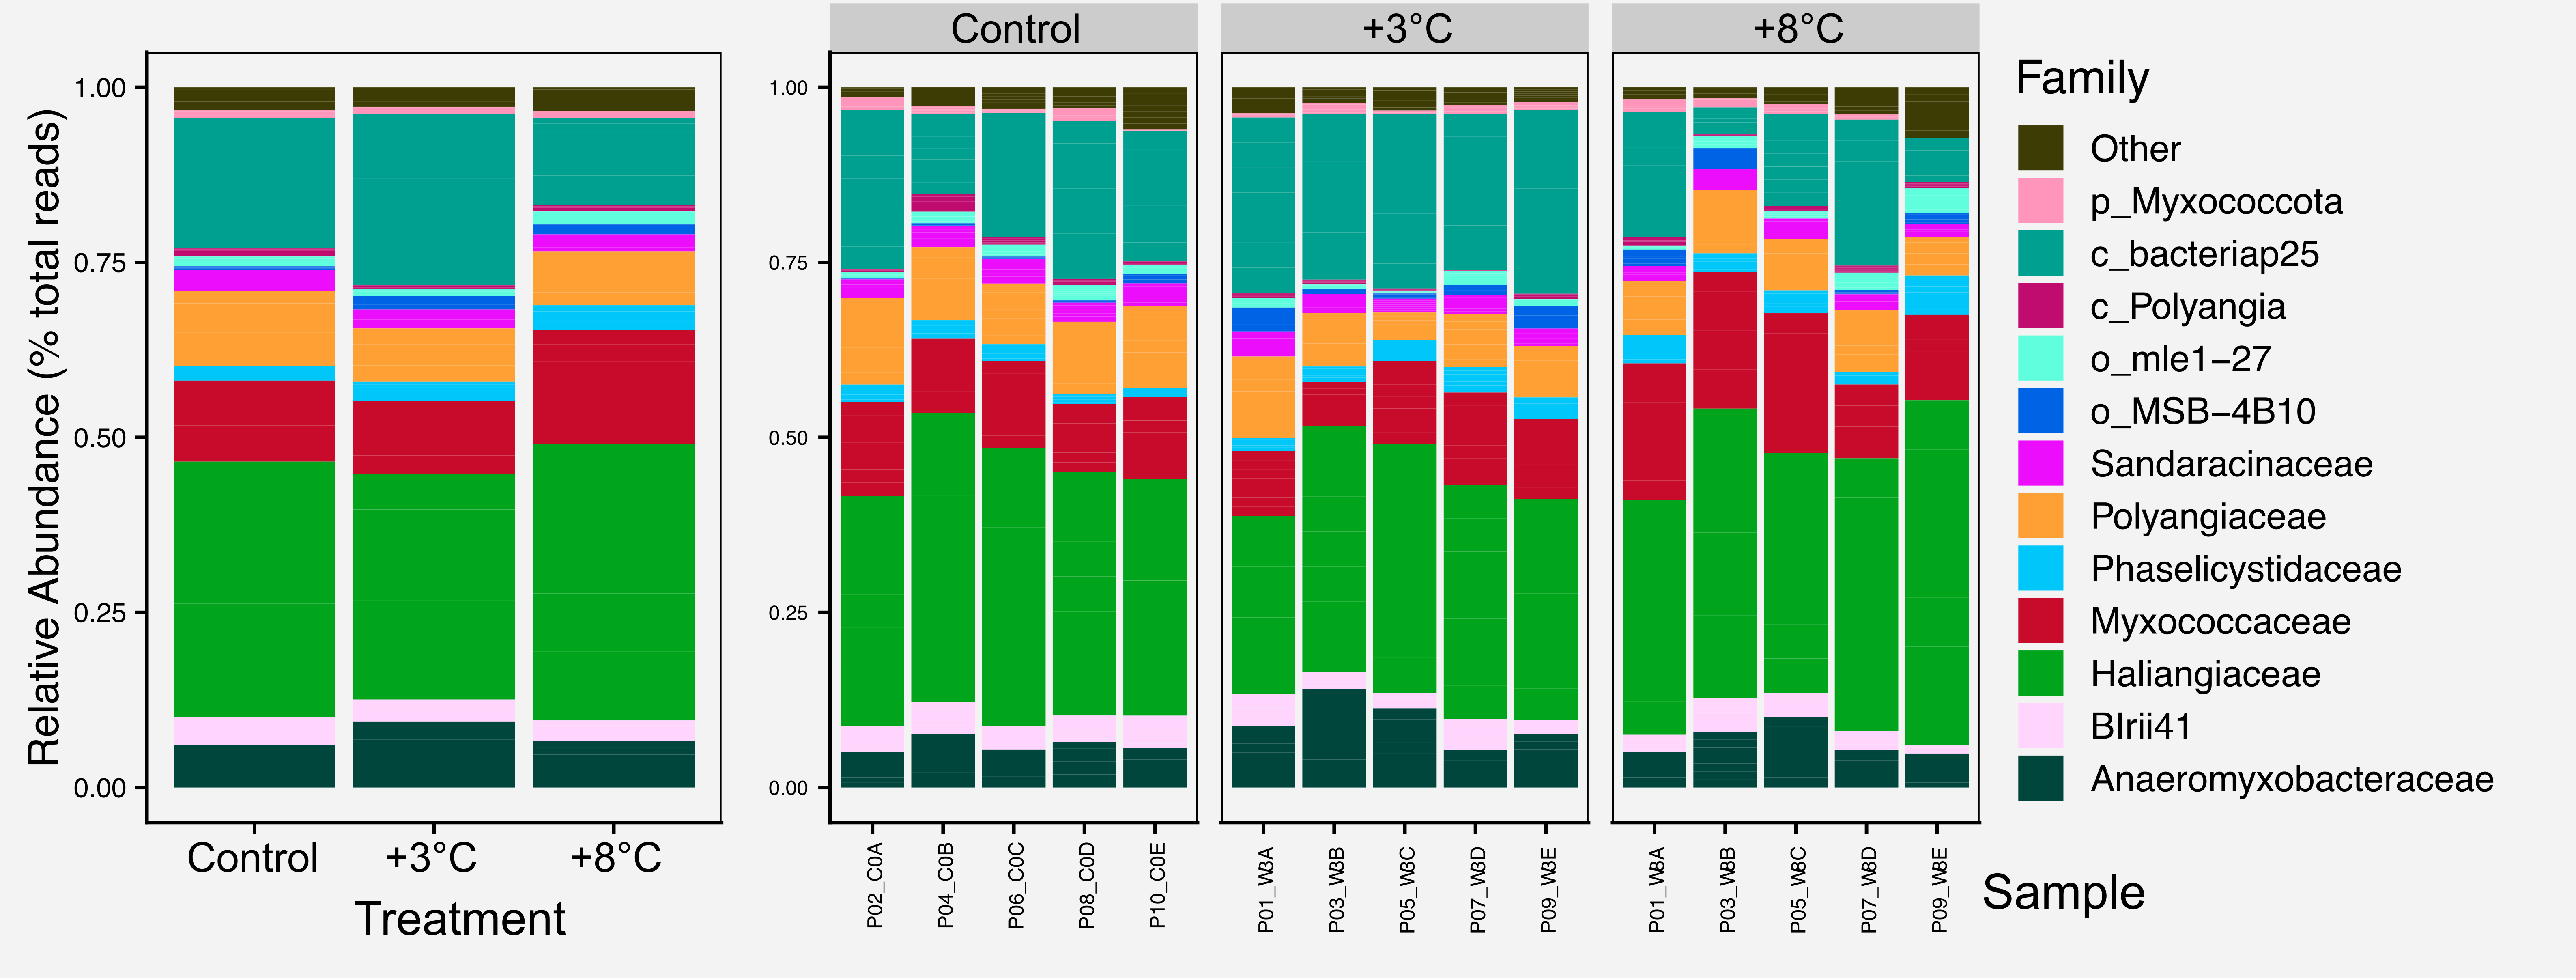
\includegraphics[width=0.95\textwidth,height=\textheight]{FIGURES/taxa_plots_class_Myxo.png}

}

\caption{\textbf{Supplementary Figure 13 |} Myxococcota family plots.}

\end{figure}

\begin{figure}

{\centering 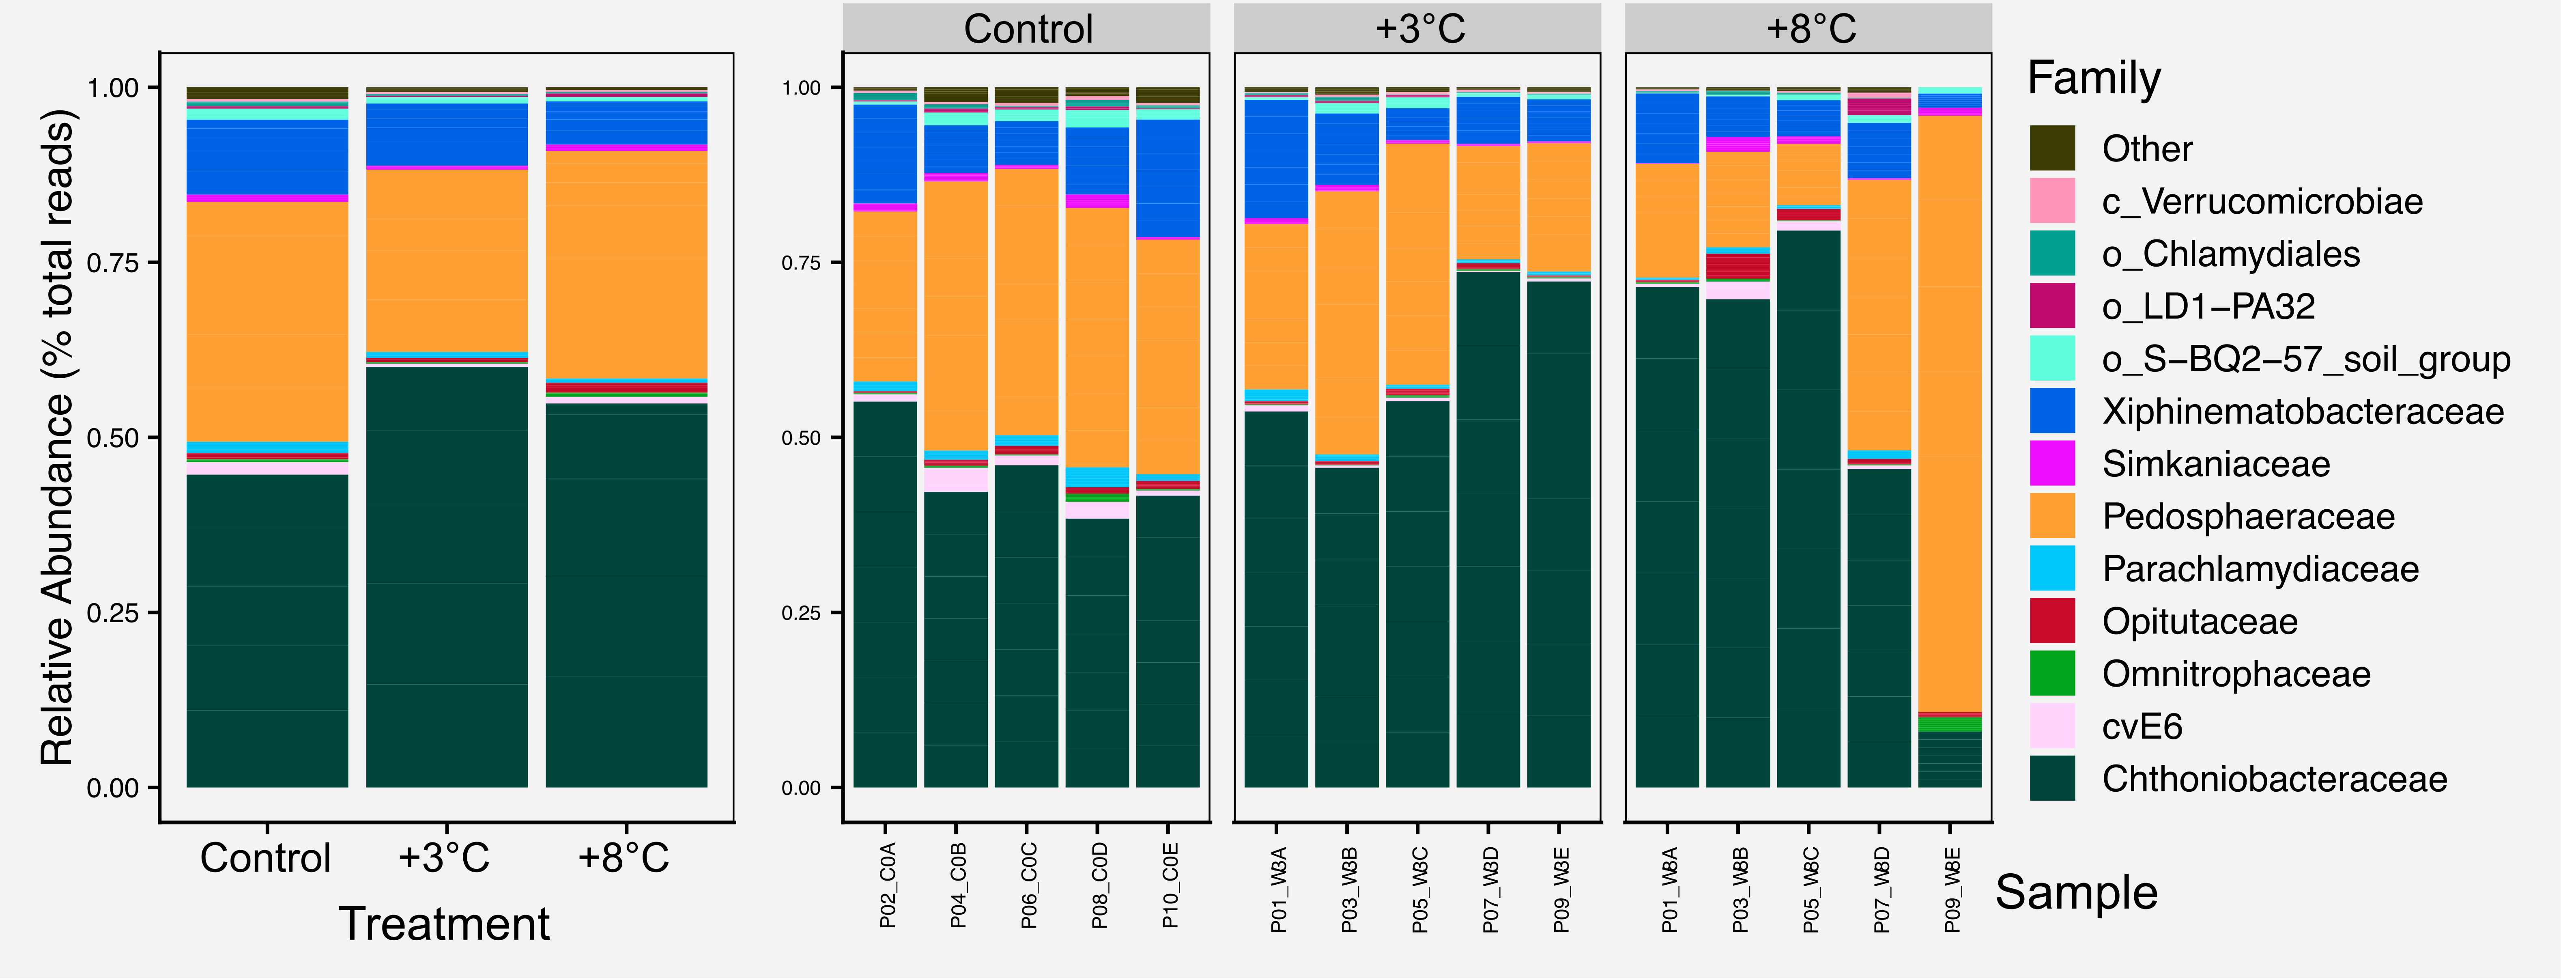
\includegraphics[width=0.95\textwidth,height=\textheight]{FIGURES/taxa_plots_class_Verruco.png}

}

\caption{\textbf{Supplementary Figure 14 |} Verrucomicrobiota family
plots}

\end{figure}

\newpage{}

\hypertarget{references}{%
\section{References}\label{references}}

\hypertarget{refs}{}
\begin{CSLReferences}{0}{0}
\leavevmode\vadjust pre{\hypertarget{ref-caporaso2011global}{}}%
\CSLLeftMargin{1. }%
\CSLRightInline{Caporaso, J. G. \emph{et al.}
\href{https://doi.org/10.1073/pnas.1000080107}{Global patterns of 16S
rRNA diversity at a depth of millions of sequences per sample}.
\emph{Proceedings of the National Academy of Sciences} \textbf{108},
4516--4522 (2011).}

\leavevmode\vadjust pre{\hypertarget{ref-gardes1993its}{}}%
\CSLLeftMargin{2. }%
\CSLRightInline{Gardes, M. \& Bruns, T. D.
\href{https://doi.org/10.1111/j.1365-294X.1993.tb00005.x}{ITS primers
with enhanced specificity for basidiomycetes-application to the
identification of mycorrhizae and rusts}. \emph{Molecular Ecology}
\textbf{2}, 113--118 (1993).}

\leavevmode\vadjust pre{\hypertarget{ref-white1990amplification}{}}%
\CSLLeftMargin{3. }%
\CSLRightInline{White, T. J., Bruns, T., Lee, S., Taylor, J., \emph{et
al.} Amplification and direct sequencing of fungal ribosomal RNA genes
for phylogenetics. \emph{PCR protocols: a guide to methods and
applications} \textbf{18}, 315--322 (1990).}

\leavevmode\vadjust pre{\hypertarget{ref-martin2011cutadapt}{}}%
\CSLLeftMargin{4. }%
\CSLRightInline{Martin, M.
\href{https://doi.org/10.14806/ej.17.1.200}{Cutadapt removes adapter
sequences from high-throughput sequencing reads}. \emph{EMBnet. journal}
\textbf{17}, 10--12 (2011).}

\leavevmode\vadjust pre{\hypertarget{ref-callahan2016dada2}{}}%
\CSLLeftMargin{5. }%
\CSLRightInline{Callahan, B. J. \emph{et al.}
\href{https://doi.org/10.1038/nmeth.3869}{DADA2: High-resolution sample
inference from illumina amplicon data}. \emph{Nature Methods}
\textbf{13}, 581 (2016).}

\leavevmode\vadjust pre{\hypertarget{ref-team2013r}{}}%
\CSLLeftMargin{6. }%
\CSLRightInline{Team, R. C. \href{https://www.R-project.org/}{R: A
language and environment for statistical computing}.}

\leavevmode\vadjust pre{\hypertarget{ref-wang2007naive}{}}%
\CSLLeftMargin{7. }%
\CSLRightInline{Wang, Q., Garrity, G. M., Tiedje, J. M. \& Cole, J. R.
\href{https://doi.org/10.1128/AEM.00062-07}{Naive bayesian classifier
for rapid assignment of rRNA sequences into the new bacterial taxonomy}.
\emph{Applied and Environmental Microbiology} \textbf{73}, 5261--5267
(2007).}

\leavevmode\vadjust pre{\hypertarget{ref-quast2012silva}{}}%
\CSLLeftMargin{8. }%
\CSLRightInline{Quast, C. \emph{et al.}
\href{https://doi.org/10.1093/nar/gks1219}{The SILVA ribosomal RNA gene
database project: Improved data processing and web-based tools}.
\emph{Nucleic Acids Research} \textbf{41}, D590--D596 (2012).}

\leavevmode\vadjust pre{\hypertarget{ref-nilsson2019unite}{}}%
\CSLLeftMargin{9. }%
\CSLRightInline{Nilsson, R. H. \emph{et al.}
\href{https://doi.org/10.1093/nar/gky1022}{The UNITE database for
molecular identification of fungi: Handling dark taxa and parallel
taxonomic classifications}. \emph{Nucleic Acids Research} \textbf{47},
D259--D264 (2019).}

\leavevmode\vadjust pre{\hypertarget{ref-abarenkov2020unite}{}}%
\CSLLeftMargin{10. }%
\CSLRightInline{Abarenkov, K. \emph{et al.}
\href{https://dx.doi.org/10.15156/BIO/786368}{UNITE general FASTA
release for fungi}. (2020).}

\leavevmode\vadjust pre{\hypertarget{ref-mcmurdie2013phyloseq}{}}%
\CSLLeftMargin{11. }%
\CSLRightInline{McMurdie, P. J. \& Holmes, S.
\href{https://doi.org/10.1371/journal.pone.0061217}{Phyloseq: An r
package for reproducible interactive analysis and graphics of microbiome
census data}. \emph{PLoS One} \textbf{8}, e61217 (2013).}

\leavevmode\vadjust pre{\hypertarget{ref-smirnova2019perfect}{}}%
\CSLLeftMargin{12. }%
\CSLRightInline{Smirnova, E., Huzurbazar, S. \& Jafari, F.
\href{https://doi.org/10.1093/biostatistics/kxy020}{PERFect: PERmutation
filtering test for microbiome data}. \emph{Biostatistics} \textbf{20},
615--631 (2019).}

\leavevmode\vadjust pre{\hypertarget{ref-roesch2020pime}{}}%
\CSLLeftMargin{13. }%
\CSLRightInline{Roesch, L. F. W. \emph{et al.}
\href{https://doi.org/10.1111/1755-0998.13116}{PIME: A package for
discovery of novel differences among microbial communities}.
\emph{Molecular Ecology Resources} \textbf{20}, 415--428 (2020).}

\leavevmode\vadjust pre{\hypertarget{ref-alberdi2019guide}{}}%
\CSLLeftMargin{14. }%
\CSLRightInline{Alberdi, A. \& Gilbert, M. T. P.
\href{https://doi.org/10.1111/1755‐0998.13014}{A guide to the
application of hill numbers to DNA-based diversity analyses}.
\emph{Molecular Ecology Resources} \textbf{19}, 804--817 (2019).}

\leavevmode\vadjust pre{\hypertarget{ref-alberdi2019hilldiv}{}}%
\CSLLeftMargin{15. }%
\CSLRightInline{Alberdi, A. \& Gilbert, M. T. P.
\href{https://doi.org/10.1101/545665}{Hilldiv: An r package for the
integral analysis of diversity based on hill numbers}. \emph{bioRxiv}
545665 (2019).}

\leavevmode\vadjust pre{\hypertarget{ref-balint2016millions}{}}%
\CSLLeftMargin{16. }%
\CSLRightInline{Bálint, M. \emph{et al.}
\href{https://doi.org/10.1093/femsre/fuw017}{Millions of reads,
thousands of taxa: Microbial community structure and associations
analyzed via marker genes}. \emph{FEMS Microbiology Reviews}
\textbf{40}, 686--700 (2016).}

\leavevmode\vadjust pre{\hypertarget{ref-roswell2021conceptual}{}}%
\CSLLeftMargin{17. }%
\CSLRightInline{Roswell, M., Dushoff, J. \& Winfree, R.
\href{https://doi.org/10.1111/oik.07202}{A conceptual guide to measuring
species diversity}. \emph{Oikos} \textbf{130}, 321--338 (2021).}

\leavevmode\vadjust pre{\hypertarget{ref-shapiro1965analysis}{}}%
\CSLLeftMargin{18. }%
\CSLRightInline{Shapiro, S. S. \& Wilk, M. B.
\href{https://doi.org/10.2307/2333709\%20}{An analysis of variance test
for normality (complete samples)}. \emph{Biometrika} \textbf{52},
591--611 (1965).}

\leavevmode\vadjust pre{\hypertarget{ref-bartlett1937properties}{}}%
\CSLLeftMargin{19. }%
\CSLRightInline{Bartlett, M. S.
\href{https://doi.org/10.1098/rspa.1937.0109}{Properties of sufficiency
and statistical tests}. \emph{Proceedings of the Royal Society of
London. Series A-Mathematical and Physical Sciences} \textbf{160},
268--282 (1937).}

\leavevmode\vadjust pre{\hypertarget{ref-oksanen2013community}{}}%
\CSLLeftMargin{20. }%
\CSLRightInline{Oksanen, J. \emph{et al.}
\href{https://cran.r-project.org/web/packages/vegan/index.html}{Vegan:
Community ecology package}. \emph{R package version} \textbf{2},
(2012).}

\leavevmode\vadjust pre{\hypertarget{ref-chen2012associating}{}}%
\CSLLeftMargin{21. }%
\CSLRightInline{Chen, J. \emph{et al.}
\href{https://doi.org/10.1093/bioinformatics/bts342}{Associating
microbiome composition with environmental covariates using generalized
UniFrac distances}. \emph{Bioinformatics} \textbf{28}, 2106--2113
(2012).}

\leavevmode\vadjust pre{\hypertarget{ref-fuglede2004jensen}{}}%
\CSLLeftMargin{22. }%
\CSLRightInline{Fuglede, B. \& Topsoe, F. Jensen-shannon divergence and
hilbert space embedding. in \emph{International symposium on information
theory, 2004. ISIT 2004. proceedings.} 31 (IEEE, 2004).}

\leavevmode\vadjust pre{\hypertarget{ref-bray1957ordination}{}}%
\CSLLeftMargin{23. }%
\CSLRightInline{Bray, J. R. \& Curtis, J. T.
\href{https://doi.org/10.2307/1942268\%20}{An ordination of the upland
forest communities of southern wisconsin}. \emph{Ecological Monographs}
\textbf{27}, 326--349 (1957).}

\leavevmode\vadjust pre{\hypertarget{ref-legendre2011testing}{}}%
\CSLLeftMargin{24. }%
\CSLRightInline{Legendre, P., Oksanen, J. \& ter-Braak, C. J.
\href{https://doi.org/10.1111/j.2041-210X.2010.00078.x}{Testing the
significance of canonical axes in redundancy analysis}. \emph{Methods in
Ecology and Evolution} \textbf{2}, 269--277 (2011).}

\leavevmode\vadjust pre{\hypertarget{ref-legendre1999distance}{}}%
\CSLLeftMargin{25. }%
\CSLRightInline{Legendre, P. \& Anderson, M. J.
\href{https://doi.org/10.1890/0012-9615(1999)069\%5B0001:DBRATM\%5D2.0.CO;2}{Distance-based
redundancy analysis: Testing multispecies responses in multifactorial
ecological experiments}. \emph{Ecological Mmonographs} \textbf{69},
1--24 (1999).}

\leavevmode\vadjust pre{\hypertarget{ref-clarke1993non}{}}%
\CSLLeftMargin{26. }%
\CSLRightInline{Clarke, K. R.
\href{https://doi.org/10.1111/j.1442-9993.1993.tb00438.x}{Non-parametric
multivariate analyses of changes in community structure}.
\emph{Australian Journal of Ecology} \textbf{18}, 117--143 (1993).}

\leavevmode\vadjust pre{\hypertarget{ref-gower1966some}{}}%
\CSLLeftMargin{27. }%
\CSLRightInline{Gower, J. C.
\href{https://doi.org/10.1093/biomet/53.3-4.325}{Some distance
properties of latent root and vector methods used in multivariate
analysis}. \emph{Biometrika} \textbf{53}, 325--338 (1966).}

\leavevmode\vadjust pre{\hypertarget{ref-roberts2016package}{}}%
\CSLLeftMargin{28. }%
\CSLRightInline{Roberts, D. W. \& Roberts, M. D. W.
\href{https://cran.r-project.org/web/packages/labdsv/index.html}{Package
{`labdsv'}}. \emph{Ordination and Multivariate} \textbf{775}, (2016).}

\leavevmode\vadjust pre{\hypertarget{ref-cao2020package}{}}%
\CSLLeftMargin{29. }%
\CSLRightInline{Cao, Y.
\href{https://doi.org/10.5281/zenodo.3749415}{microbiomeMarker:
Microbiome biomarker analysis}. \emph{R package version}
\textbf{0.0.1.9000}, (2020).}

\leavevmode\vadjust pre{\hypertarget{ref-segata2011metagenomic}{}}%
\CSLLeftMargin{30. }%
\CSLRightInline{Segata, N. \emph{et al.}
\href{https://doi.org/10.1186/gb-2011-12-6-r60}{Metagenomic biomarker
discovery and explanation}. \emph{Genome Biology} \textbf{12}, 1--18
(2011).}

\leavevmode\vadjust pre{\hypertarget{ref-peterson2019ordered}{}}%
\CSLLeftMargin{31. }%
\CSLRightInline{Peterson, R. A. \& Cavanaugh, J. E.
\href{https://doi.org/10.1080/02664763.2019.1630372}{Ordered quantile
normalization: A semiparametric transformation built for the
cross-validation era}. \emph{Journal of Applied Statistics} (2019).}

\leavevmode\vadjust pre{\hypertarget{ref-peterson2021finding}{}}%
\CSLLeftMargin{32. }%
\CSLRightInline{Peterson, R. A. Finding optimal normalizing
transformations via bestNormalize. \emph{The R Journal} (2021).}

\leavevmode\vadjust pre{\hypertarget{ref-mantel1967detection}{}}%
\CSLLeftMargin{33. }%
\CSLRightInline{Mantel, N. The detection of disease clustering and a
generalized regression approach. \emph{Cancer Research} \textbf{27},
209--220 (1967).}

\leavevmode\vadjust pre{\hypertarget{ref-legendre2012numerical}{}}%
\CSLLeftMargin{34. }%
\CSLRightInline{Legendre, P. \& Legendre, L. \emph{Numerical ecology}.
(Elsevier, 2012).}

\leavevmode\vadjust pre{\hypertarget{ref-faith1987compositional}{}}%
\CSLLeftMargin{35. }%
\CSLRightInline{Faith, D. P., Minchin, P. R. \& Belbin, L.
\href{https://doi.org/10.1007/BF00038687}{Compositional dissimilarity as
a robust measure of ecological distance}. \emph{Vegetatio} \textbf{69},
57--68 (1987).}

\end{CSLReferences}



\end{document}
